%Preámbulo
\documentclass[11pt,titlepage]{report}
\usepackage[spanish]{babel}
\usepackage[utf8]{inputenc} 
\usepackage[T1]{fontenc}
\usepackage{lmodern}
\usepackage[tmargin =1.25in, lmargin=1.25in, rmargin=1.25in, bmargin=1.25in]{geometry}
\usepackage{placeins}
\usepackage{titlesec, lscape, graphicx}
\usepackage[hidelinks]{hyperref} 
\usepackage{subfig} %dos figuras juntas
\usepackage{wrapfig} %se escribe a la par de la figura
\usepackage{fancyhdr}
\usepackage{cite, amsmath, caption}
\usepackage{chronosys}
\usepackage{tikz,times,ifthen}
\usepackage{verbatim}
\usepackage{smartdiagram}
\usetikzlibrary{arrows.meta, chains, fit, positioning, shapes.arrows}
\usetikzlibrary{mindmap,trees,backgrounds}
\definecolor{color_mate}{RGB}{255,255,128}
\definecolor{color_plas}{RGB}{255,128,255}
\definecolor{color_text}{RGB}{128,255,255}
\definecolor{color_petr}{RGB}{255,192,192}
\definecolor{color_made}{RGB}{192,255,192}
\definecolor{color_meta}{RGB}{192,192,255}
\usepackage{wrapfig}
\usepackage{multicol}


\usetikzlibrary{calc,shadings,shadows}
\pagestyle{fancy}
% encabezados
\lhead[\thepage]{\rightmark}
\chead[]{}
\rhead[CAPÍTULO \thechapter. \leftmark]{\thepage}
\renewcommand{\headrulewidth}{0.5pt}

% pie de pagina
\lfoot[]{Metodología BI}
\cfoot[]{}
\rfoot[]{UNAH}
\renewcommand{\footrulewidth}{0pt}

\title{Metodología de inteligencia de negocios con aplicación: cuadro de mandos universitarios}
\author{Lester Armando Vallecillo M}
\date{24 de Febrero del 2021}
\renewcommand{\headrulewidth}{0.4pt} % grosor de la cabecera
\usepackage{chngcntr}
\counterwithout{footnote}{chapter}
%cuenta todos los indices sin empezar un nuevo conteo en el siguinete capitulo

% ****************************************************

%definir condiciones de estilo del documento
\renewcommand{\baselinestretch}{1.5} %Interlineado 1.5
\rm %definir el tipo de letra en Roman

\titleformat{\chapter}{\normalfont\huge}{\thechapter.}{14pt}{\huge\it}
  
%\renewcommand*\thesection{\arabic{section}}
%\renewcommand*\thesubsection{\arabic{subsection}}
\begin{document}
	
%%%%%%%%%%%%% PORTADA %%%%%%%%%%%%%%%%%%%%%%
\begin{titlepage}
  \vspace*{1cm}
\begin{center}
\huge{\textbf{Una metodología estándar de inteligencia de negocios (BI) con aplicación: cuadro de mando universitario}}
\end{center}
\hrule

 \begin{center}
	{\LARGE{UNIVERSIDAD NACIONAL AUTÓNOMA DE HONDURAS}}\\
	{\LARGE \textbf{Escuela de Matemáticas}}\\[0.4cm] 
	
\includegraphics[height=4.5cm]{Figuras/UNAH}\\[0.3cm]
 	{\LARGE\underline{Proyecto de Investigación}}\\ 
 \end{center}
\begin{center}
	\begin{list}{}{}
	\item \begin{center}
		\textbf{Autor:}
	\end{center}
	\item \begin{center}
		Lester Armando Vallecillo Montoya
	\end{center}
	\item \begin{center}
		\textbf{Supervisor:}
	\end{center}
	\item \begin{center}
		MSc. Iván Henríquez\\
		Jefe Departamento de Matemática Aplicada\\[1.6cm]
	\end{center}
\end{list}
\end{center}
   {\large Tegucigalpa, Honduras, C.A. \hfill 24 de Febrero del 2021}
\end{titlepage}


%%%%%%%%%%% ABSTRACT %%%%%%%%%%%%%%%%%
\begin{abstract}

{\LARGE A}nalizar la información para transformarla en conocimiento de manera eficiente, es un reto para las organizaciones de la actualidad. La inteligencia de negocios (BI, Business Intelligence) surge como un arma estratégica para descubrir ventajas competitivas en el mercado, utilizando el conocimiento que describe la información oportuna mediante el uso de herramientas de análisis de datos para dar soporte a la toma de decisiones.\\

En el contexto académico, se pretende describir algunos conceptos teóricos y prácticos, que se utilizan para desarrollar modelos de gestión de información o de negocios mediante una solución BI, con mayor énfasis en una metodología de implementación estándar. Por tanto, es importante explorar la teoría de los tres pilares de la inteligencia empresarial: BI, analítica de negocios (BA, Business Analytics) y big data (BD). Específicamente, se presentan algunos modelos y algoritmos de los campos de estudio: matemática, estadística e informática, además del uso práctico de los cuadro de mando (DW, Dashwoard) con la medición de indicadores de rendimiento (KPIs, Key Performance Indicator). De la misma manera, se refiere a la transferencia de conocimiento, técnicas y tecnologías (Know how) disponibles para la integración de la información, automatización de tareas (Workflow), enfoques metodológicos y visualización de datos.\\


Prácticamente, es importante desarrollar un proyecto mediante el enfoque de necesidad táctica para implementar la metodología estándar que proporcione una solución BI, a los requerimientos socializados por parte de usuarios finales de las diferentes unidades administrativas u operativas de las universidades. En conclusión, con un prototipo de BI se pretende validar la investigación presentando un modelo generativo denominado <<cuadro de mando universitario>>.\\

         
\paragraph{Palabras Clave:}	
Inteligencia, negocios, analítica, integración, datos, información, toma de decisiones, modelo, automatización, KPIs, informe, cuadro de mando, metodología, enfoque, proceso, estrategia, herramientas, aplicaciones y tecnologías.
\end{abstract}
\pagenumbering{roman}

%  ********************************
%    AGRADECIMIENTO 
%%%%%%%%%%%%%%%%%%%%%%%%%%%%%%%%%%%
\newpage
\thispagestyle{empty}
\vspace*{5cm}
\section*{Agradecimiento}
En primera instancia, agradezco a Dios por darle un propósito a mi vida, del cual se cumple en parte, con este trabajo de investigación. Ciertamente, fue una etapa muy provechosa, sobretodo de aprendizaje y superación profesional.\\

En segunda instancia, le doy gracias a mi ángel, abuela y madre de crianza Elisa Serrano, pues a ella le debo todo lo positivo que hay en mi como ser humano, además de mi tía Delfina Serrano, quien fue la primer persona que tuvo fe en mi para el estudio, hoy no están para verme cosechar la semilla que ellas sembraron, pero se que estarían orgullosas y alegres por mi. En conclusión, a ellas dedico este nuevo escalón de éxito en mi vida. Y en fin, le agradezco  a mis padres y familia en general, por su apoyo económico, moral y espiritual.\\

Luego, le agradezco a mis amigos y compañeros laborales que en algún momento me apoyaron en el ámbito profesional. Finalmente, agradezco a los catedráticos de la carrera de matemáticas, quienes me inspiraron a seguir creciendo profesionalmente, sobretodo por sus enseñanzas académicas, consejos y ejemplo de modelo a seguir.

%  ********************************
%    TÓPICOS 
%%%%%%%%%%%%%%%%%%%%%%%%%%%%%%%%%%%
\newpage
\thispagestyle{empty}
\vspace*{2cm}
\section*{Tópicos}
\begin{list}{}
\item “Hay un tiempo cuando debemos elegir firmemente el camino que seguiremos, o la deriva implacable de los acontecimientos \textbf{tomará las decisiones}”
\begin{flushright}
\textit{Franklin D Roosevelt}
\end{flushright}
	\vspace*{0.4cm}
	\item “Como se obtenga, administre y \textbf{use la
		información}, podremos determinar si
	ganamos o perdemos”
	\begin{flushright}
		\textit{Bill Gates}
	\end{flushright}
	\vspace*{0.4cm}
	\item “Si miras cualquier tipo de organización
	moderna y piensas ‘¿Cuál es el
	\textbf{instrumento de poder} mas potente’?,
	verás que es la información”
	\begin{flushright}
		\textit{Ricardo Semler}
	\end{flushright}
	\vspace*{0.4cm}
	\item “Los clientes no esperan que seas
	perfecto. Esperan que les aportes
	\textbf{soluciones} cuando tienen algún problema”
	\begin{flushright}
		\textit{Michael Porter}
	\end{flushright}
\end{list}
\pagebreak


%%%%%%%%%% INDICE %%%%%%%%%%%%%%%%%
\tableofcontents


%%%%%%%%%%% INTRODUCCIÓN %%%%%%%%%%%%%%%%%
\chapter{INTRODUCCIÓN}

\section{Introducción}
Ciertamente, la solución al problema de tener mucha información y no saber traducirla en conocimiento es todo un reto. En este sentido, las organizaciones con ó sin fines de lucro cuentan con un sistema de gestión de información para dar soporte a sus actividades administrativas y operativas. Esto induce una idea,  “con el tiempo las aplicaciones llegan a tener la historia de la organización y los datos almacenados en las bases de datos, pueden ser utilizados para argumentar la decisión que se quiera tomar ante cualquier aspecto para mejora en la organización” (Rosado Gomez, 2010). Lo anterior sugiere, explotar la información para extraer conocimientos y resultados que permitan mejorar la toma de decisiones.\\

En particular, la inteligencia de negocios (BI) se presenta como una alternativa dinámica para ese fin, mediante la integración de los datos. Sin embargo, para extraer conocimiento de los datos se complementa con analitica de negocios (BA), y ocasionalmente por big data (BD), los otros dos pilares de la inteligencia empresarial.\\

Por su parte, NewVantage Partners realizo encuestas anuales sobre los ejecutivos y su percepción de los datos. En resumen, los resultados demuestran que ellos están utilizando análisis de datos y obtienen los resultados esperados, pero hasta 2018 solamente el 33\% logró crear una cultura de datos. También, son pesimistas con la disrupción de la inteligencia artificial (AI, Artificial Intelligence) que cada día adoptan las grandes corporaciones. De ellos, el 80\% teme que empresas especializadas en big data (BD) se desplacen a su mercado generando competencia, además un 13\% teme a computación en la nube, entre otras disrupciones \cite{art06}. Por tanto, se propone la BI para dar solución a los requerimientos de información con oportunidad y gestionar el uso eficaz de los datos.\\

En efecto, BI es una disciplina que ha ido evolucionando y adaptándose a la evolución tecnológica de la información (IT), la cual se implemento por tendencias innovadoras en las organizaciones empresariales. De la misma manera, la analítica de negocios (BA, Business Analytics) es una disciplina complementaria que se apoya en técnicas de analítica de datos \cite{lib02}.\\

Para fines académicos, de lo anterior se sugiere exponer algunos fundamentos de BI basados en la toma de decisiones estratégicas y operativas, como la medición de indicadores del rendimiento (KPIs) utilizando un enfoque metodológico. Adicionalmente, será necesario explorar el uso práctico del cuadro de mando integral (BSM, Balanced Scorecard Methodology) y de algunas herramientas, aplicaciones y tecnologías de BI. En conclusión, es importante desarrollar un prototipo de proyecto destinado para ejecutar análisis de datos y apoyar la toma de decisiones, designadas a la unidad organizativa.


%  ********************************
%    GLOSARIO 
%%%%%%%%%%%%%%%%%%%%%%%%%%%%%%%%%%%
\newpage
\section{Glosario de términos}
\begin{table}[h]
\begin{tabular}{ll}
AI\label{AI} & Artificial Intelligence, Inteligencia Artificial\\
BA\label{BA} & 	Business Analytics, Analítica de negocios\\
BBDD\label{BaseD} & Abreviatura de base de datos\\
BI\label{BI} & 	Business Intelligence, Inteligencia de negocios\\
BD\label{BD}  & Big Data, Conjuntos de datos de mayor variabilidad, volumen y velocidad\\
BSM\label{BSM} & Balanced Scorecard Methodology, Cuadro de mando integral\\
DASHWOARD\label{DW}  & Control, Cuadro ó tablero de mando\\
DA\label{DA}  & Data Analytics, Analítica de datos\\
DATA MART\label{DMart} &  Almacén particular de datos con una finalidad concreta\\
DSS\label{DSS}& Decision Support System, Sistema de soporte a las decisiones\\
DWH\label{DWH}  & Data Warehouse, Depósito general de datos\\
DM\label{DM}  & Data Mining, Prospección ó Minería de datos\\
DMo\label{DMo}  & Dimensional modeling, Modelado dimensional\\
ERP\label{ERP}  & Es un planificador de recursos. Automatiza tareas y procesos BI\\
ETL\label{ETL}  & Proceso de extracción, transformación y carga de los datos\\
HEURÍSTICA\label{HEU} & Proceso destinado a guiar la toma de decisiones\\
KH\label{KH} & Know-How,  Se refiere a transferencia de conocimientos, técnicas ó tecnologías\\
KPIs\label{KPI} &  key performance indicator, Indicadores claves del rendimiento\\
ML\label{ML} & Machine Learning, Aprendizaje automático\\
METODOLOGÍA\label{MET} &  Conjunto de métodos que sigue una investigación científica\\
OLAP\label{OLAP} &  Procesamiento analítico en línea en estructuras dimensionales\\
TI\label{TI}  &   Tecnología de información para almacenar y manipular datos\\
WF\label{WF} & Workflow, se refiere a la automatización de las tareas de una organización
\end{tabular}
\end{table}

%  ********************************
%     PLANTEAMIENTO DEL PROBLEMA %%%%%%%%%%%%%%%%%%%%%%%%%%%%%%%%%%%  

\chapter{PLANTEAMIENTO DEL PROBLEMA} 
\pagenumbering{arabic}

En este capítulo, se expone la problemática que inspiro al nacimiento de nuevas herramientas de análisis de datos utilizadas en las organizaciones, principalmente de negocios, y además se formulan los objetivos de su implementación. De la misma manera, se justifica la demanda de una metodología BI con la finalidad de darle sentido a la transferencia de conocimientos, técnicas ó tecnologías (Know-How). Posteriormente, se describe el alcance que conlleva la implementación de metodologías por parte del planificador de recursos empresariales (ERP, Enterprise Resource Planning) y finalmente, se delimita el planteamiento del problema a un modelo encargado de gestionar la información.


%  ********************************
%     PRECEDENTES
 %%%%%%%%%%%%%%%%%%%%%%%%%%%%%%%%%%%
\section{Precedentes}
La necesidad de crear herramientas con la capacidad de transformar los datos operacionales en información y luego en conocimiento por parte de las organizaciones, permite la aparición de BI con la idea de mejorar y optimizar los procesos de los negocios aprovechando la tecnología para implantar la automatización de tareas de una organización (Workflow).\\

En 1962, Kenneth Iverson realiza el primer avance significativo y denominado OLAP (On-Line Analytical Processing) como el primer lenguaje de programación multidimensional y que forma la base del procesamiento analítico en línea \cite{web01}. Sin embargo, esta tecnología fue incorporada hasta los 90' por las grandes corporaciones.\\

En 1969, Edgar Codd creó el concepto de base de datos, pero fue hasta los 70' que surgieron los primeros modelos de bases de datos y relacionales para la gestión operacional de negocios.\\

En los 80' surge el concepto de Data Warehouse (DWH) y se estandariza el lenguaje SQL. En resumen, esto fue un punto de inflexión en la tecnología de información (TI), ya que soluciono la dificultad en la implementación de DWH. Sin embargo, era necesario diseñar nuevas herramientas de análisis porque no se podía comparar, ni adaptar un modelo DWH con un sistema transaccional OLTP \cite{tes01}.\\

Posteriormente, en 1989, Howard Dresner, propuso la inteligencia de negocios (BI) para definir una metodología que permitiera mejorar la toma de decisiones empresariales \cite{web02}.\\

Consecuentemente, la idea de Dresner se materializo a principios de los 90', con la creación de Business Intelligence 1.0 (BI) y múltiples aplicaciones que ofrecían acceso a bases de datos distribuidas en la arquitectura cliente/servidor, y en general a la información estructurada generada por las empresas, pero todavía incapaces de analizar grandes volúmenes de datos.\\

Para inicio del nuevo milenio, evoluciona el Business Intelligence  a una versión 2.0 (BI 2.0) y se consolidan las aplicaciones BI en plataformas, tomando en cuenta la información no estructurada y centralizada \cite{web01}. Simultáneamente, se destaca Social BI con capacidad de integración de datos externos en relación con la información de la empresa.\\

En la actualidad, se mantiene la tradicional BI, pero los grandes volúmenes de datos requieren de nuevas herramientas para su integración \cite{web01}. Esto, permite la evolución de BI a nuevas soluciones capaces de analizar la información de manera rápida y eficiente, principalmente Big Data. Finalmente, algunas organizaciones comienzan a hacer uso de los datos para dar soporte a la toma de decisiones.


\begin{figure}[h]
	\caption{Evolución de BI. [Fuente: Propia]}
	\centering
	\resizebox{\linewidth}{!}{% Resize table to fit within
		\begin{tikzpicture}[]
		%draw horizontal line
		\draw (0,0) -- (41/1.7,0);
		%draw vertical lines
		\foreach \x in {0, 8, 16, 24, 32, 40}{
			\draw (\x/1.7,3pt) -- (\x/1.7,-3pt);
		}
		%draw nodes
		\draw (0,0) node[below=3pt]{\textbf{OLAP}} node[above=3pt]{60'};
		\draw (8/1.7,0) node[below=3pt] {\textbf{BBDD}} node[above=3pt]{70'};
		\draw (16/1.7,0) node[below=3pt] {\textbf{DWH}} node[above=3pt] {80'};
		\draw (24/1.7,0) node[below=3pt] {\textbf{BI 1.0}}  node[above=3pt] {90'};
		\draw (32/1.7,0) node[below=3pt] {\textbf{BI 2.0}} node[above=3pt] {2000'};
		\draw (40/1.7,0) node[below=3pt] {\textbf{BI - Big Data}} node[above=3pt] {Actualidad};
					
		\end{tikzpicture}
	}
	\label{fig:evolucionBI}
\end{figure}

%  ********************************
  
%  ********************************
%     DEFINICIÓN DEL PROBLEMA %%%%%%%%%%%%%%%%%%%%%%%%%%%%%%%%%%%

\section{Definición del Problema}
Cada día, en las organizaciones aumenta la necesidad de hacer uso eficaz de la información y desarrollar una cultura de datos, ante las situaciones que se presentan,  pero la constante urgencia es darle sentido al conocimiento que describen los datos de manera implícita. En síntesis, este problema consiste en implementar procesos metodológicos utilizando las herramientas, aplicaciones y tecnologías de análisis de datos disponibles, de manera que se cumplan los objetivos estratégicos. Los problemas más comunes que describe \cite{gui02} son:
\begin{multicols}{2}
	\begin{itemize}
		\item Diferentes versiones de los echos
		\item  Incapacidad para realizar análisis y presentar información importante
		\item  Necesidad de una tecnología más simple y fácil de utilizar
		\item  No existen practicas de uso y conservación de datos
		\item  Flexibilidad operativa limitada por falta de tecnología adecuada
		\item  Incapacidad para diferenciar y priorizar problemas 
		\item  No hay alineación de los objetivos estratégicos y operativos
	\end{itemize}
\end{multicols}

Por otra parte, los metamodelos generativos persiguen generar ideas mediante el razonamiento lógico para resolver problemas. Para ilustrar este concepto, se presentan algunos ejemplos de problemas de aplicación BI planteados mediante preguntas (metamodelos genéricos), los cuales se describen a continuación \cite{web07}:
\begin{multicols}{2}
\textit{Venta de productos:}
\begin{itemize}
\item Quiénes son los mejores clientes?
\item Cómo se puede minimizar costos? 
\item Cuál será el pronóstico de ventas?
\end{itemize}

\textit{Gestión de una biblioteca:}
\begin{itemize}
\item Cuál es el tema más consultado?
\item Horarios con mayor concurrencia?
\item Cuales libros deben ser adquiridos?
\end{itemize}

\textit{Planificación académica:}
\begin{itemize}
	\item Como es el rendimiento académico?
	\item Como mejorar el desempeño del personal?
	\item Cuales cursos deben ser aperturados?
\end{itemize}
\end{multicols}
 
%  ********************************
%     OBJETIVOS DE LA INVESTIGACIÓN %%%%%%%%%%%%%%%%%%%%%%%%%%%%%%%%%%%


\section{Objetivos de la Investigación}

Generalmente, las organizaciones se centran en analizar la información desde un enfoque practico de las operaciones. De la misma manera, para obtener resultados positivos es necesario implementar técnicas y tácticas en función de los objetivos específicos. Principalmente, es prioridad incorporar las necesidades estratégicas que permiten plantear el objetivo general.

\subsection{Objetivo General}
El objetivo general de esta investigación es presentar una metodología estándar que permite desarrollar proyectos de inteligencia de negocios mediante un enfoque teórico y practico con orientación a la toma de decisiones estratégica y operativa en las organizaciones. En consecuencia del objetivo general, se derivan algunos objetivos específicos.

\subsection{Objetivos Específicos}
\begin{multicols}{2}
\begin{description}

\item[Implementar] una metodología estándar de inteligencia de negocios que permita generar conocimiento para dar soporte a la toma de decisiones.

\item[Investigar] los modelos y algoritmos matemático/estadístico e informáticos utilizados para desarrollar inteligencia empresarial.

\item[Generar] conocimiento para sustentar evidencia de las teorías científicas y fomentar una cultura de datos en las organizaciones.
	
\item[Automatizar] actividades de análisis de datos como informes, cuadros de mando, tareas en la nube y consultas de información.

\item[Integrar] la información de las diferentes fuentes de datos utilizando modelos de datos diseñados para gestionar la información.

\item[Utilizar] las herramientas, aplicaciones y tecnologías de inteligencia de negocios para el análisis y visualización de la información.

\item[Exponer] la importancia de la inteligencia de negocios, específicamente para analizar diferentes escenarios, determinar tendencias y proyectar datos.

\item[Validar] la metodología estándar mediante el desarrolló de un prototipo denominado <<control de mando universitario>>.
\end{description}
\end{multicols}


%  ********************************
%     JUSTIFICACIÓN 
%%%%%%%%%%%%%%%%%%%%%%%%%%%%%%%%%%%

\section{Justificación}

Normalmente, en el análisis de datos se presentan inconsistencias en la integración de los sistemas de información entre si, lo cual provoca representar los macrodatos de forma aislada \cite{gui01}. De la misma manera, las aplicaciones que presentan los informes finales saturan los macrodatos u omiten información relevante para el análisis. Algunas características que limitan dichos sistemas son las siguientes:

\begin{itemize}
\item Rigidez para la extracción de datos
\item Largo tiempo de respuesta
\item Falta de integración de datos
\item Datos inconsistentes o incompletos
\item Adecuación de la información a usuarios
\item Falta de información histórica
\end{itemize}

Por lo tanto, es indispensable definir un proceso metodológico de análisis de datos basado en el método científico para su correcta implementación y retroalimentación de procesos recurrentes y permanentes de un proyecto de gestión de información. Se podría implementar una metodología de inteligencia de negocios? Curto Díaz \& Conesa Caralt, resaltaron algunas situaciones en las que será nesesario desarrollar proyectos de inteligencia de negocios.
\begin{itemize}
\item La toma de decisiones se realiza de manera intuitiva
\item Automatización de los procesos de recopilación de información
\item La información no es efectiva
\item Problemas de calidad y repositorios de información
\item Exceso de información para ser analizada
\item Necesidad de cruzar información entre unidades organizativas
\end{itemize}

%  ********************************
%     ALCANCE: MODELO GENERATIVO 
%%%%%%%%%%%%%%%%%%%%%%%%%%%%%%%%%%%

\section{Alcance}
Técnicamente, el propósito de esta investigación es plantear problemas mediante metamodelos generativos para desarrollar modelos de gestión de la información (modelos de negocios). Es decir, un sistema de evaluación adecuado que ayudará al usuario final, específicamente al personal ejecutivo a mejorar la toma de decisiones operativas, enfocar a la gerencia a decidir sobre la ejecución de planificación estratégica. Por su parte, los metamodelos generativos implican las situaciones siguientes:

\begin{itemize}
	\item Situaciones sin números
	\item Información para deducir algo
	\item Situaciones cualitativas
	\item Enunciados abiertos
\end{itemize}

Literalmente, se puede generalizar el procedimiento de un modelo generativo/predictivo que gestione la información de los negocios a partir de las preguntas formuladas mediante metamodelos genéricos de los requerimientos que se derivan del planteamiento del problema. En segunda instancia, se identifica la información disponible en los datos obtenidos para luego, gestionar el conocimiento mediante la analítica de datos. Finalmente, se desarrolla un modelo general que resume la información de los diferentes modelos de gestión del conocimiento y que representan situaciones reales dentro de las organizaciones. Está idea se ilustra en la Figura \ref{fig:modeloGestionN}.

\begin{figure}[h]
	\centering
	\resizebox{\linewidth}{!}{% Resize table to fit within
	\begin{tikzpicture}[ node distance = 10mm and 6mm,
	start chain = A going right, force/.style = {rectangle, rounded corners, draw, fill=cyan!30, inner sep=4mm, outer sep=0mm, minimum size=8mm, font=\bfseries\sffamily, on chain},
	CA/.style = {% Connection Arrow
		single arrow, draw, single arrow head extend=2mm,
		minimum height=5mm, minimum width=3mm, outer sep=1mm},
	LA/.style = {% Long Arrow 
		CA, draw=none, left color=cyan!20, right color=cyan,
		inner xsep = 10mm, minimum width=9mm, label=center:#1,}]

\newline
\begin{scope}[every node/.style={force}]
\node   {Metamodelos};     % A-1
\node   {Información};
\node   {Conocimiento};
\node   { Gestión };
\node   { Modelos };
\end{scope}
	% arrows between nodes
	
	\node[CA, above=0mm of A-1] {Problemas};
	\node[CA, above=0mm of A-2] {Datos};
	\node[CA, above=0mm of A-3] {Modelo de datos};
	\node[CA, above=0mm of A-4] {Analítica de datos};
	\node[CA, above=0mm of A-5] { Negocios };
	% long arrows with text
	\coordinate[below=of A-1]   (a1);

	\node[LA= Modelo Generativo/Predictivo,
	fit=(a1) (a1 -| A-5)] {};
	
	\end{tikzpicture} }
\caption{Procedimiento del modelo de gestión de la información. [Fuente: Propia]} \label{fig:modeloGestionN}	
\end{figure}

% **********************************
%  ********************************
%    MARCO TEÓRICO 
%%%%%%%%%%%%%%%%%%%%%%%%%%%%%%%%%%%
\chapter{MARCO TEÓRICO} 

Este capítulo se centra en comprender los principales componentes estructurales de una solución utilizada para desarrollar modelos de gestión de la información mediante una metodología estándar de implementación de inteligencia de negocios (BI) para organizaciones lucrativas o no. Y para fines académicos, se considera importante conocer sobre algunos conceptos de modelos, técnicas, métodos y algoritmos de matemática, informática, estadística avanzada y analítica de negocios.

%  ********************************
%   MODELOS DE GESTIÓN DE INFORMACIÓN 
%%%%%%%%%%%%%%%%%%%%%%%%%%%%%%%%%%%
\newpage
\section{La necesidad de la información}

\begin{verbatim}
Que hacer ante la nesesidad de gestionar la información?
\end{verbatim}\\

Ante la necesidad de soluciones a la problemática expuesta en el capitulo anterior, en las organizaciones se presentan situaciones que implican la necesidad de información oportuna para proporcionar soluciones empresariales mediante el uso adecuado de herramientas, aplicaciones y tecnologías de inteligencia de negocios (BI), y así, dar certeza en la veracidad de la información. Por lo tanto, como solución a esta problemática se pueden desarrollar diferentes modelos de gestión de la información o de negocios, utilizando herramientas de analítica de datos (DA) con la finalidad de generar conocimiento oportuno para dar soporte a la toma de decisiones estratégicas y operativas en las organizaciones.\\

\section{La gestión del conocimiento}

Ciertamente, la época actual se aproxima a una cuarta revolución industrial (industria 4.0) que también se denominada 'la era digital' y ahora, las organizaciones requieren de realizar una gestión adecuada de los datos y su correcta interpretación \cite{art03}.\\

 Es decir, optimizar los procesos y establecer modelos, según sea la necesidad del análisis para encontrar resultados al alcance de los problemas planteados y representarlos a través de conceptos lógicos como los metamodelos genéricos.\\ 

Contemporáneamente, con la industria 4.0 se desarrollo una explosión de fuentes de datos estructurados y no estructurados como internet, redes sociales, telefonía móvil y los macrodatos generados con herramientas,  aplicaciones y tecnologías. Pero estas, ahora disponen de una mayor capacidad de almacenamiento y cálculo, lo cual permite mejorar la gestión del conocimiento \cite{art04}.\\

\begin{wrapfigure}{c}{0.5\linewidth}
	\scalebox{0.8}{
		\smartdiagram[connected constellation diagram]{Sistema BI, Datos, Desición, Conocimiento, Información} }
	\caption{Proceso cíclico de un sistema BI. [Fuente: Propia]} \label{fig: DSS}
\end{wrapfigure}

En síntesis, el conocimiento generado por la información se extrae de las fuentes de datos que utilizan los usuarios para guiar la toma de decisiones utilizando procesos de heurística o sistemas de decisión (DSS, Decision Support System) y están destinados a gestionar los negocios en las organizaciones, esté proceso cíclico hace referencia a una solución o sistema BI utilizado para gestionar los negocios de la organización, como se ilustra intuitivamente en la Figura \ref{fig: DSS}.\\ \\


\subsection{Los modelos de gestión}

La finalidad de los modelos de gestión o de negocios es generar las soluciones de inteligencia empresarial que genera el sistema BI a través de un modelo de datos. Estrategicamente, las organizaciones desarrollan esquemas de planificación cuya finalidad es proporcionar resultados concretos de las diferentes áreas operativas y administrativas, las cuales usan el modelo de información para gestionar los negocios.\\

En retrospectiva, es necesario convertir los datos en información valiosa que normalmente se pueden tomar de cada unidad operativa ó administrativa de la organización, como se ilustra con el ejemplo del Cuadro \ref{Cuadro: ModelosG}. 

\begin{table}[h]
\begin{tabular}{| l | l | l |}
\hline
\textbf{UNIDAD}&\textbf{\ DATOS} &\textbf{\ MODELOS DE GESTIÓN \ } \\ \hline
Ventas  & \begin{tabular}[c]{@{}l@{}} Productos\\ Clientes \\ Pedidos\end{tabular}  & \begin{tabular}[c]{@{}l@{}}Productos rentables \\ Clientes mayoritarios \\ Proyección de ventas \end{tabular} \\
\hline
Marketin  & \begin{tabular}[c]{@{}l@{}}Campañas\\ Encuestas\end{tabular} & \begin{tabular}[c]{@{}l@{}}Campañas estrategicas\\ Clientes potenciales\end{tabular} \\
\hline
Facultad            &  \begin{tabular}[c]{@{}l@{}} Alumnos \\ Cursos\end{tabular}                             &  \begin{tabular}[c]{@{}l@{}} Exelencia academica \\ Carga academica\end{tabular}  \\
\hline
Servicio al cliente & \begin{tabular}[c]{@{}l@{}}Llamadas de clientes\\ Información actualizada\end{tabular} & \begin{tabular}[c]{@{}l@{}}Cumplimiento de metas\\ Canales de ventas exitosos\\ Consultas frecuentes\end{tabular}                            \\
\hline
Logistica  & \begin{tabular}[c]{@{}l@{}}Productos recibidos\\ Productos solicitados\\ Tiempo de entrega\end{tabular} & \begin{tabular}[c]{@{}l@{}}Gestión de pedidos retrasados\\ Seguimiento de la entrega\end{tabular}   \\ \hline
\end{tabular} 
\caption{Ejemplos de modelos de gestión de negocios}
\label{Cuadro: ModelosG}
\end{table}

\newpage
\subsection{Modelo Generativo/Predictivo}

Generalmente, en la práctica los científico de datos desarrollan modelos de negocios basados en situaciones que resumen los históricos de datos. Sin embargo, esto se puede clasificar en dos tipos de modelos como las culturas del modelaje que propone Leo Breiman \cite{art05}:

\begin{description}
	\item[Modelado generativo:] que propone un modelo estocástico que podría haber generado los datos y usa métodos para inferir propiedades generativas subyacentes. Usualmente, coincide con las estadísticas académicas tradicionales y  describe el tiempo presente.
	 
	\item[Modelado predictivo:] se constituye por un conjunto de métodos de predicción de los datos. Normalmente, converge con el aprendizaje automático (ML, Machine Learning) y describe el tiempo futuro.
\end{description}

Finalmente, este conjunto de modelos de gestión de negocios integran un modelo general que resume la información y que se define como el modelo generativo o predictivo.


%  ********************************
%   LA ANALITICA DE DATOS PARA LA TOMA DE DESICIONES 
%%%%%%%%%%%%%%%%%%%%%%%%%%%%%%%%%%%
\section{Analítica de negocios (BA)}

Generalmente, las organizaciones están adoptando la analítica de negocios (BA, Business Analytics), pero la mayoría aun no ha formado una cultura en base al conocimiento de la información \cite{art06}. Estadisticamente, en las organizaciones el 93\% de los gerentes sienten presión para tomar decisiones en cortos periodos de tiempo, el 62\% admite no haber recibido la información oportuna para tomar decisiones y el 88\% admite utilizar su intuición el 75\% de las situaciones que toman decisiones de negocios.\\

En definición, BA es un conjunto de técnicas y herramientas utilizadas para analizar datos preparados y almacenados en depósitos, que permite dar seguimiento a los procesos empresariales mediante aplicaciones BI, principalmente de analítica y minería de datos y métodos empresariales como los cuadros de mando integral que además, utilizan indicadores de desempeño (KPIs).

\subsection{Analítica de datos (DA)}
Técnicamente, la analítica de datos es el análisis sistemático que utiliza datos históricos para descubrir patrones y tendencias. Básicamente, se desarrolla mediante los análisis descriptivo, predictivo y prescriptivo, este ultimo, se basa en investigación de operaciones, técnicas o métodos de matemáticas y de estadísticas avanzada. Este procedimiento básico se ilustra en la Figura \ref{fig: analitica}.

\begin{figure}[h]
	\centering
	\resizebox{\linewidth}{!}{% Resize table to fit within
		\begin{tikzpicture}[ node distance = 10mm and 6mm,
		start chain = A going right, force/.style = {rectangle, rounded corners, draw, fill=cyan!30, inner sep=2mm, outer sep=0mm, minimum size=8mm, font=\bfseries\sffamily, on chain},
		CA/.style = {% Connection Arrow
			single arrow, draw, single arrow head extend=2mm,
			minimum height=5mm, minimum width=3mm, outer sep=1mm},
		LA/.style = {% Long Arrow 
			CA, draw=none, left color=cyan!20, right color=cyan,
			inner xsep = 10mm, minimum width=9mm, label=center:#1,}]
		\newline
		\begin{scope}[every node/.style={force}]
		\node   {Análisis Descriptivo};     % A-1
		\node   {Análisis Predictivo};
		\node   {Análisis Prescriptivo};
		\end{scope}
		% arrows between nodes
		\node[CA, above=0mm of A-1] {Qué ha pasado?};
		\node[CA, above=0mm of A-2] {Qué va pasar?};
		\node[CA, above=0mm of A-3] {Qué debería hacer?};
	
		\end{tikzpicture} }
	\caption{Procedimiento básico de analítica de datos. [Fuente: Propia]} \label{fig: analitica}	
\end{figure}

Según Turban (2011), las aplicaciones más utilizadas en BA son visualizaciones de datos como informes (reports) que incluye reportes estáticos y dinámicos mediante análisis de datos dimensional (cubos OLAP) y las consultas (queries).


\subsection{Minería de datos (DM)}
La mineria de datos (DM, Data Minig) es un conjunto de técnicas y metodologías que se utilizan para optimizar el proceso de una solución BI, específicamente se centra en identificar relaciones desconocidas o patrones en bases de datos mediante herramientas como métodos de estadística avanzada, aprendizaje automático (ML) e inteligencia Artificial (AI). Técnicamente, puede ser usada con propósitos descriptivos o predictivos utilizando los algoritmos de análisis supervisado y no supervisado, que integran los modelos de aprendizaje \cite{lib02}. Por ejemplo, la metodología de los modelos analíticos CRISP-DM (Cross Industry Standard Process for Data Mining) y SEMMA (Sample Explore Modlfly Model Asses) de minería de datos se pueden resumir en seis fases como se ilustra en las Figuras \ref{fig: CRISP} y \ref{fig: SEMMA}, respectivamente.

\begin{figure}[h]
\centering
\resizebox{\linewidth}{!}{% Resize table to fit within
\begin{tikzpicture}
\tikzset{ bound/.style={ draw, minimum height=2cm, inner sep=1em, },
arrow/.style={ draw, minimum height=1cm, inner sep=1em, shape=signal,
				signal from=west, signal to=east,
				signal pointer angle=110, 		} 		}
\node[bound] (a) {Negocios};
\begin{scope}[start chain=transition going right,node distance=-\pgflinewidth]
\node[arrow,right=1cm of a,on chain] {Datos};
\node[arrow,on chain] {Preparación};
\node[arrow,on chain] {Modelado};
\node[arrow,on chain] {Evaluación};
\end{scope}
\node[bound,right=1cm of transition-end]{Implantación};	
\end{tikzpicture}}
\caption{Procedimiento del modelo CRISP-DM. [Fuente: Propia]} \label{fig: CRISP}	
\end{figure} 

\hrule
\begin{figure}[h]
\centering
\resizebox{\linewidth}{!}{% Resize table to fit within
\begin{tikzpicture}
\tikzset{ bound/.style={
				draw, minimum height=1.5cm, inner sep=1em, 	},
			arrow/.style={ draw, minimum height=1cm, inner sep=1em,
				shape=signal, signal from=west, signal to=east,
				signal pointer angle=110, 		} 		}
\node[bound] (a) {{ Muestreo}};
\begin{scope}[start chain=transition going right,node distance=-\pgflinewidth]
\node[arrow,right=1cm of a,on chain] { Exploración};
\node[arrow,on chain] { Modificación};
\node[arrow,on chain] { Modelado};
\end{scope}
\node[bound,right=1cm of transition-end]{ Evaluación};	
\end{tikzpicture} }
\caption{Procedimiento del modelo SEMMA. [Fuente: Propia]} \label{fig: SEMMA}	
\end{figure} 

\subsubsection{Algoritmos de aprendizaje}
Se refiere al uso de algoritmos en los modelos de aprendizaje. Particularmente, los modelos descriptivos que se apoyan en aprendizaje no supervisado \cite{lib02}. Por su parte, las técnicas predictivas más utilizadas por estos modelos son los algoritmos siguientes:

\begin{multicols}{2}
\begin{itemize}
\item Clasificación
\item Regresión
\item Series temporales
\item Detección de anomalías
\end{itemize}
\end{multicols}

Además, los modelos predictivos se apoyan en aprendizaje supervisado. Las técnicas descriptivas más utilizadas son los algoritmos siguientes:
\begin{multicols}{2}
\begin{itemize}
\item Asociación
\item Segmentación (clustering)
\item Sumarización (resúmenes)
\item Descubrimiento de patrones
\end{itemize}
\end{multicols}


\subsection{Indicadores claves del rendimiento (KPIs)}

Utilizar análisis de datos para dar soporte a la toma de decisiones por parte de gerentes, requiere de utilizar una variedad de métodos empresariales que definen los procesos para dar seguimiento y así, cumplir con los objetivos estratégicos. Esto se conoce como administración del rendimiento gerencial \cite{lib02}. Es otras palabras, es un conjunto de aplicaciones y metodologías que forman parte de la evolución de Bl y comprende la monitorización mediante indicadores claves del rendimiento (KPIs, Key Performance Indicator) para la medición del desempeño en las organizaciones. Los procesos se gestionan en base a los objetivos estratégicos, como se ilustra en la Figura \ref{fig: KPIs}.

\begin{figure}[h]
	\centering
	\resizebox{\linewidth}{!}{% Resize table to fit within
		\begin{tikzpicture}
		\tikzset{ bound/.style={ draw, minimum height=2cm, inner sep=1em, },
			arrow/.style={ draw, minimum height=1cm, inner sep=1em, shape=signal, signal from=west, signal to=east,
				signal pointer angle=110, 		} 		}
		\node[bound] (a) {Visión};
		\begin{scope}[start chain=transition going right,node distance=-\pgflinewidth]
		\node[arrow,right=1cm of a,on chain] {Estrategias};
		\node[arrow,on chain] {Objetivos};
		\node[arrow,on chain] {Actuación operativa};
				\end{scope}
		\node[bound,right=1cm of transition-end]{Procesos};	
		\end{tikzpicture}}
	\caption{Ilustración de la gestión de procesos. [Fuente: Propia]} \label{fig: KPIs}	
\end{figure} 


\subsection{Cuadro de Mando Integral (BSM)}

\begin{wrapfigure}{c}{0.47\linewidth}
	\scalebox{1}{
		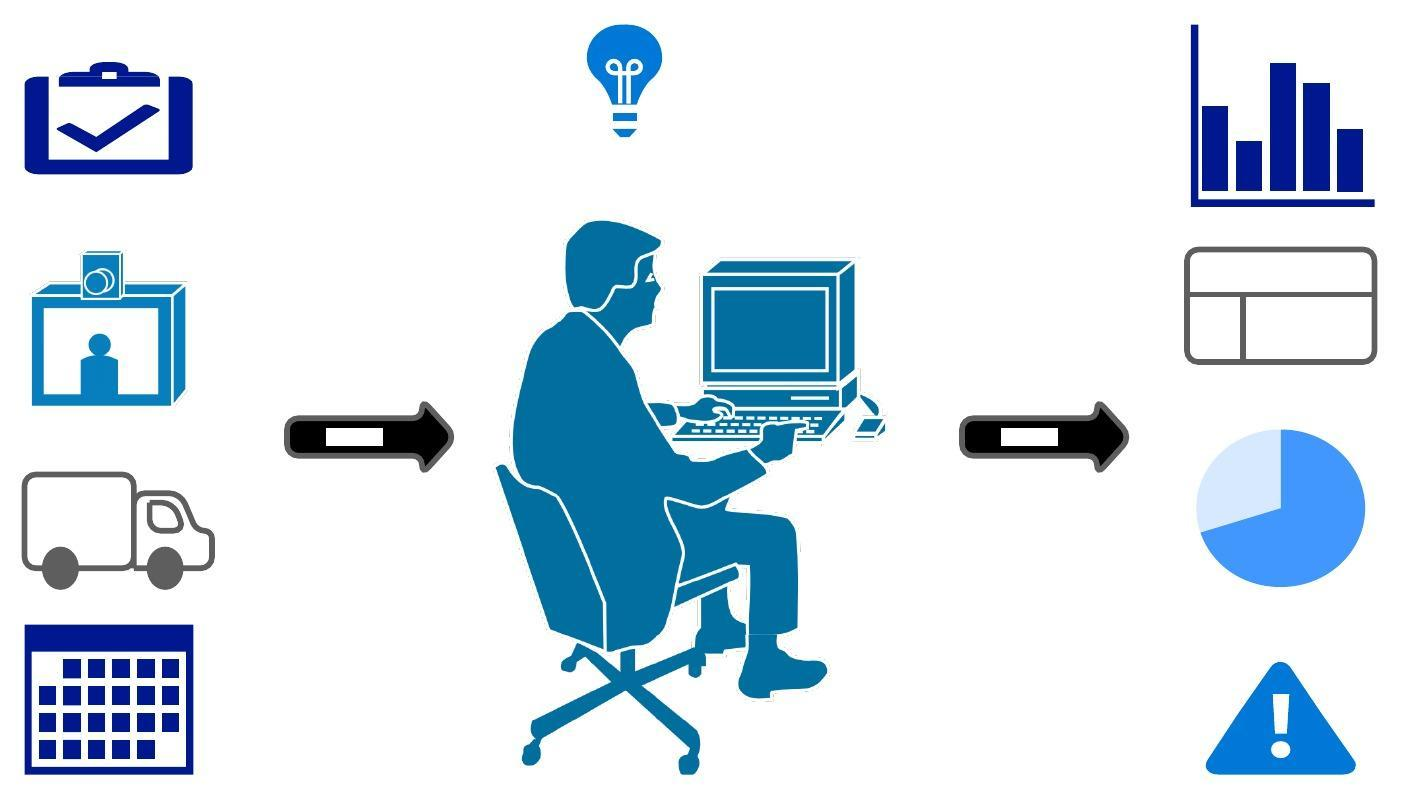
\includegraphics[width=1.1\linewidth]{Figuras/CMI} }
	\caption{Ilustración del uso de BSM. [Fuente: Propia]}
	\label{fig: starnet}
\end{wrapfigure}

Cuadro de Mando Integral (BSM, Balanced Scorecard Methodology) es la metodología más utilizada para la administración del rendimiento en las organizaciones de la actualidad y se centran en utilizar los KPIs en un entorno general de los negocios mediante el enfoque de generar competencia en el mercado \cite{lib02}. El uso principal de BSM requiere de una interfaz diseñada por herramientas de visualización de datos, tales como gráficos, tablas, cuadros de datos, alertas e informes interactivos.\\

\subsubsection{Utilidades de BSM}
En conclusión, BSM es un instrumento de gestión de negocios que facilita el funcionamiento de la estrategia organizacional. Las utilidades más comunes, según Kaplan y Norton son las siguientes:
\begin{itemize}
\item Simplificar y actualizar la estrategia
\item Comunicar la estrategia
\item Alinear las metas individuales con la estrategia
\item Vincular los objetivos a los presupuestos
\item Conducir las revisiones del funcionamiento
\end{itemize}

\subsubsection{Perceptivas de BSM}
En el proceso metodológico de BSM se pueden utilizar diferentes algoritmos de aprendizaje. Particularmente, se destaca el <<árbol de decisiones>>, en cuyos nodos se describe la acción definida y cuantificada para ejecutar la visión estratégica desde las cuatro perceptivas siguientes:
 \begin{itemize}
\item Perspectiva financiera
\item Perspectiva del cliente
\item Perspectiva de los procesos internos
\item Perspectiva de aprendizaje y crecimiento
\end{itemize}

%  ********************************
%   LA INTELIGENCIA DE NEGOCIOS (BI) 
%%%%%%%%%%%%%%%%%%%%%%%%%%%%%%%%%%%
\newpage
\section{Inteligencia de negocios (BI)}

En la actualidad, las organizaciones cuentan con sistemas de información que soportan sus actividades administrativas y operativas \cite{tes02}. En este ámbito, la inteligencia de negocios surge con un enfoque estratégico para orientar sistemáticamente el seguimiento, la comunicación y la transformación de datos con relación al débil conocimiento de la información procesable (Kamel y Samia Rouibah). Dicho enfoque, ayuda al usuario a identificar los requerimientos y se clasifica según la necesidad de información \cite{web04}:
\begin{description}
\item[Operativo:] para la toma de decisiones de las actividades diarias y operativas.

\item[Táctico:] presentar informes en ciertos periodos de tiempo y dar seguimiento a las metas.

\item[Estratégico:] se usa para gestionar los objetivos planteados por la alta dirección ó gerentes.\\

\end{description}

\def\pyramidwidth{0.7cm}
\def\pyramiddepth{0.5cm}
\def\pyramidheight{.35cm}
\def\levels{3}
\def\levelsep{0.04}
\begin{wrapfigure}{c}{0.5\linewidth} 
\scalebox{0.4}{
\begin{tikzpicture}[line width=1pt, every node/.style={scale=3},
level 1/.style={fill=yellow!70!black, draw=orange!80},
level 2/.style={fill=cyan!80, draw=cyan!60},
level 3/.style={fill=orange, draw=yellow!70!black!80},
x={(3.5mm,-1mm)}] 
\coordinate[alias=A1b] (A) at (0,0,0);
\coordinate[alias=C1b] (C) at (\pyramidwidth,0,\pyramiddepth);
\coordinate[alias=B1b] (B) at (0,0,\pyramiddepth);
\coordinate[alias=D1b] (D) at (\pyramidwidth,0,0);
\coordinate (H) at (\pyramidwidth/2,\pyramidheight,\pyramiddepth/2);
    \foreach \n in {A,B,C,D}{%
	\foreach \level[remember=\level as \lastlevel (initially 1)] in {2,...,\levels}{%
\coordinate (\n\lastlevel t) at ($(\n)!\lastlevel/\levels-\levelsep/2!(H)$);
\coordinate (\n\level b) at ($(\n)!\lastlevel/\levels+\levelsep/2!(H)$);}}
\foreach \n in {A,B,C,D}{\coordinate (\n\levels t) at (H);}
%% levels
\foreach \n in {A,B,C,D}{\coordinate (\n\levels t) at (H);}
\foreach \level in {1,...,\levels}{%
	\foreach \i/\j in {D/A, A/B, B/C, C/D}{%
		\draw[level \level, line join=round] (\i\level b) -- (\j\level b) -- (\j\level t) -- (\i\level t) -- cycle;};
	\draw[level \level, line join=round] (A\level t) -- (B\level t) -- (C\level t) -- (D\level t) -- cycle;};
\begin{scope}[every node/.style={rotate=-16,xslant=.1,above, inner sep=3pt, font=\bfseries}]
\node[scale=2] at ($(B1b)!.5!(C1b)$) {Operativa};
\node[scale=2] at ($(B2b)!.5!(C2b)$) {Táctica};
\node[scale=2] at ($(B3b)!.5!(C3b)$) {Estratégica};
\end{scope}
%
\begin{scope}[x=1cm]
\draw ($(D1b)!.5!(D1t)$) -- +(1,0) node[scale=0.7,right] {Personal operativo};
\draw ($(D2b)!.5!(D2t)$) -- +(1,0) node[scale=0.7,right] { Ejecutivos y jefes};
\draw ($(D3b)!.5!(D3t)$) -- +(1,0) node[scale=0.7,right] {Alta gerencia};
\end{scope}
\end{tikzpicture} }
\caption{Necesidad de la información.  [Fuente: Propia]} \label{fig: necesidadI}
\end{wrapfigure}

Técnicamente, es conveniente que los modelos de gestión de la información estén distribuidos jerárquicamente y asignados por los esquemas de planificación según la necesidad de información de las diferentes unidades organizativas. Por su parte, los usuarios dependen del ámbito de su responsabilidad para obtener la información que apoye su gestión como se ilustra en la Figura \ref{fig: necesidadI}. De la misma manera, cada día los sistemas BI integran los datos extraídos del sistema operacional y luego, los transforman en información valiosa para generar informes y tableros de control a nivel táctico, y posteriormente  a nivel estratégico.\\

%%%%%%%%%%%%%%%%%%%%%%%%%
\subsection{Definición}
La inteligencia de negocios o Business Intelligence (BI) es un conjunto de herramientas, aplicaciones y tecnologías que permiten integrar las fuentes de información de manera eficiente, mediante procesos metodológicos de analítica de negocios (BA) con el propósito de generar conocimiento para mejorar la toma de decisiones empresariales a nivel operativo, táctico y estratégico. Donde, el nivel se puede considera como el enfoque de aplicación, en base a la necesidad de información. Este concepto, se puede ilustrar con el mapa mental de la Figura \ref{fig: BI}. 
%  ********************************
\begin{figure}[h]
%  MAPA MENTAL DE BI
\centering
\scalebox{1}{
	\begin{tikzpicture}[mindmap,
	level 1 concept/.append style={level distance=100,sibling angle=125},
	extra concept/.append style={text=black}]
	\path[mindmap,concept color=color_mate,text=black]
	node[concept, inner sep = 0mm] {INTELIGENCIA DE NEGOCIOS}  [clockwise from=38]
	% APLICACIONES
	child[concept color= color_petr] {
		node[concept, inner sep = 2mm] {Aplicaciones}  [clockwise from=115]
		child { node[concept] {Control de mandos}}
		child { node[concept] {Analitíca de datos}}
		child { node[concept] {Inteligencia artificial} }
		child { node[concept] {Mineria de datos}}
	}
	% HERRAMIENTAS
	child[concept color=color_text] {
		node[concept, inner sep = 2mm] {Herramientas} [clockwise from=0]
		child { node[concept] {Software BI} }
		child { node[concept] {OLAP} }
		child { node[concept] {Lenguajes} }
		child { node[concept] {Metodologías} } }
	% TECNOLOGIAS
	child[concept color=color_meta] { 
		node[concept, inner sep = 2mm] {Tecnologías}  [clockwise from=-115]
		child { node[concept] {Data Warehouse} }
		child { node[concept] {Informes Ad Hoc} }     
		child { node[concept] {Fuentes de datos} }
		child { node[concept] {Datos en la nube} } };
\end{tikzpicture} }
\caption{Mapa mental de inteligencia de negocios. [Fuente: Propia]} \label{fig: BI}	
\end{figure}

Automáticamente, la integración de la información procedente de las operaciones en una plataforma BI se está convirtiendo en un factor importante para el éxito de las organizaciones \cite{gui01}. En este sentido, el propósito es aprovechar este factor para tener acceso a la información, principalmente del desempeño y resultados que permiten tomar ventajas competitivas en el mercado. Este concepto, también se puede analizar desde las perspectivas de Calzada \& Abreu: tomar decisiones rápidas, convertir datos en información y usar una aplicación relacional.\\

Adicionalmente, BI se puede definir como “el cúmulo de modelos matemáticos y metodologías de análisis que explotan los datos disponibles para generar información y conocimientos útiles para los procesos de toma de decisiones” (Garcia Reyes, 2012). En conclusión, con BI se puede mejorar la toma de decisiones en base al conocimiento que describe la información precisa y oportuna para garantizar las alternativas que son más conveniente para el éxito de la organización \cite{tes02}.


% **************** ESTRUCTURA DE BI ********************
\section{Estructura tecnológica estándar de una solución BI}

Con la finalidad de comprender la estructuración tecnológica estándar de una solución utilizada para desarrollar un modelo de gestión de la información o sistema BI, de manera oportuna y acertada por parte de los usuarios en las organizaciones \cite{web07}, se describe a continuación el proceso para proporcionar una solución de BI. El cual, sintetiza el procedimiento para desarrollar un proyecto BI, y se ilustra en la Figura \ref{fig: soluciónBI} dividido en cinco fases que se describen continuación:

\begin{description}
\item[Fase 1: Planteamiento del problema]  Esta fase consiste en plantear el problema y la necesidad de información mediante metamodelos para establecer los requerimientos específicos.

\item[Fase 2: Selección de datos] Aquí se diseña el esquema lógico de selección de datos especificados en el análisis de requerimientos.

\item[Fase 3: Desarollo del modelo de datos] En esta fase se integran los datos en un modelo mediante el análisis de datos para gestionar la información.

\item[Fase 4: Analítica de negocios] Aquí se utilizan las herramientas de analítica y minería de datos para generar el conocimiento.

\item[Fase 5: Modelo de gestión] Consiste en la explotación y automatización de la información en los diferentes modelos de gestión mediante equipos y tecnologías.

\end{description}

\begin{figure}[h]
	\centering
	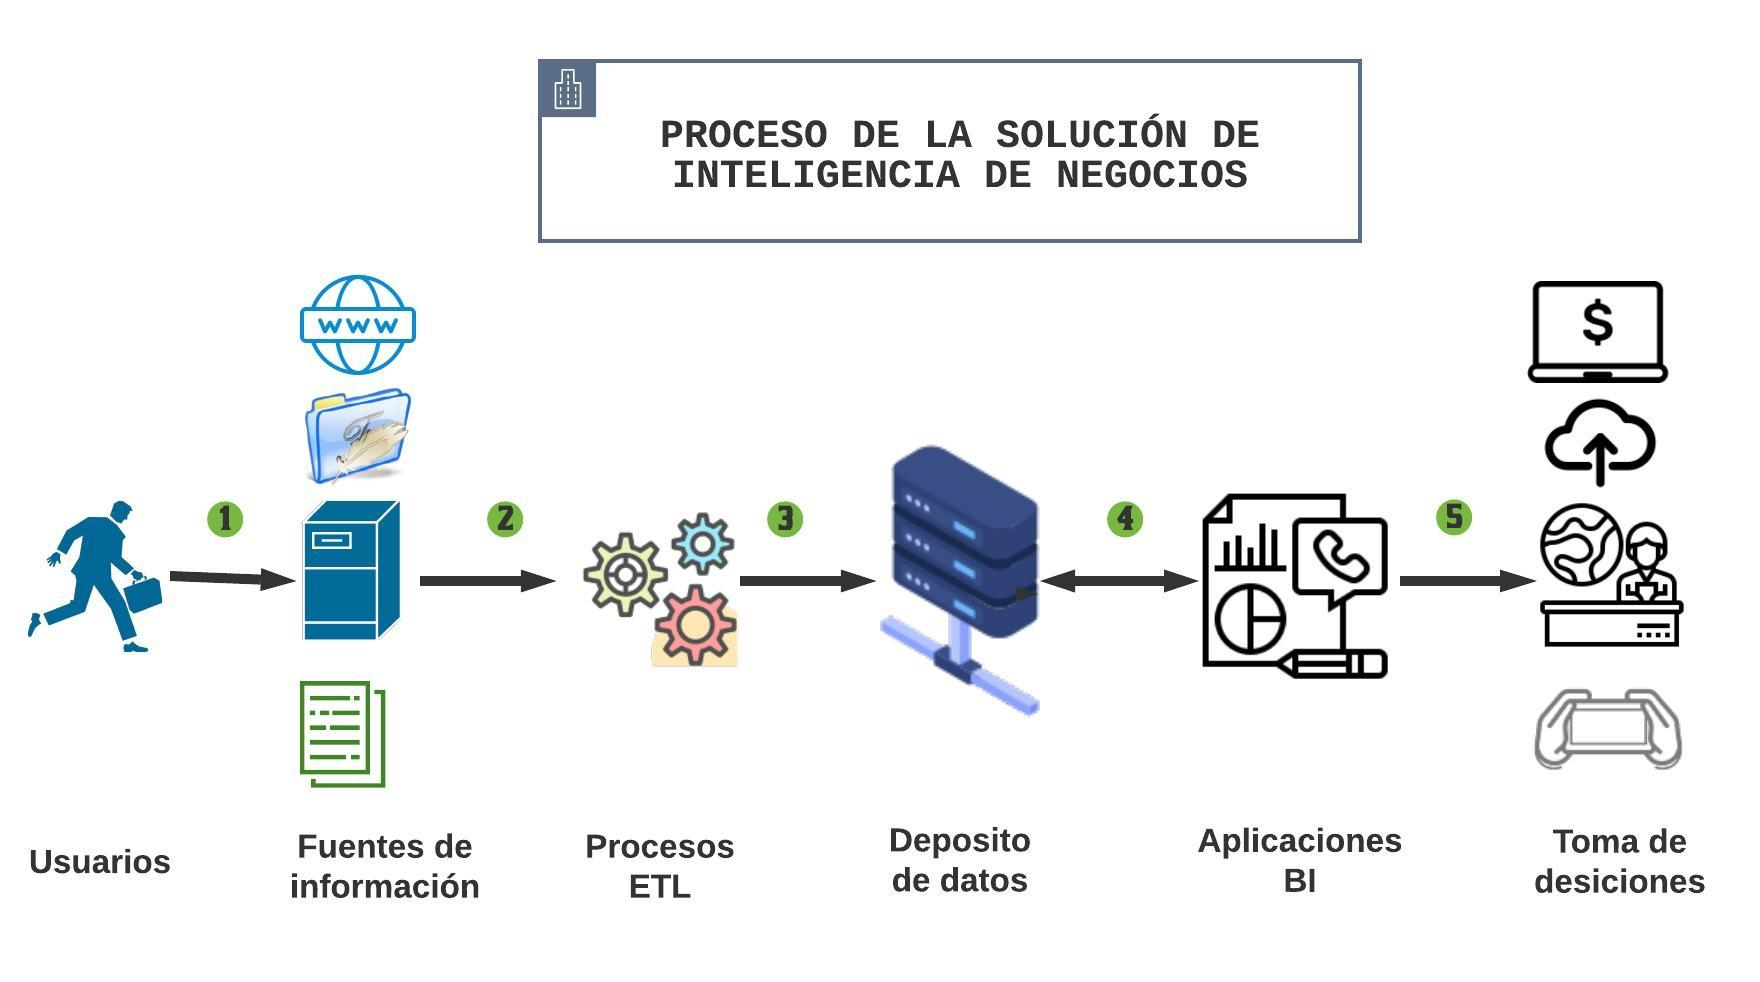
\includegraphics[width=1.05\linewidth]{Figuras/SoluBI}
	\caption{Ilustración del proceso de una solución BI estándar. [Fuente: Propia]}
	\label{fig: soluciónBI}
\end{figure}

Las cinco fases de una solución BI estándar que dividen el modelo de gestión de la información o sistema BI, forman cinco capas, como se muestra en la Figura \ref{fig: soluciónBI} y según \cite{lib02} se describen a continuación: 

\begin{description}
\item[Capa de usuarios:]  son los usuarios operativos, analistas de datos, ejecutivos, jefes y gerentes.

\item[Capa de fuentes de información:] Son las fuentes de datos estructurados o semi-estructurados al alcance de los usuarios y pueden ser de fuentes internas o externas como ser: sistemas operacionales, web, contenedores, la nube y archivos almacenados en dispositivos de información.

\item[Capa de procesos ETL:] Esta capa consume la mayor parte del tiempo y se centra tres procesos: extracción, transformación y carga de los datos. 

\item[Capa de deposito de datos:] Consta de tres componentes: almacén de
datos operacionales (ODS, Operational Data Store), los Data Marts (DM) que almacenan datos corporativos e integran el deposito de datos descrito como Data Warehouse (DWH) \cite{lib02}.\\

William H. Inmon, describió un DWH como una colección de datos orientada a un tema específico, integrado, variante en el tiempo y no volátil, que soporta el proceso de toma de decisiones. En contraste, los DWH almacenan datos en una estructura dimensional (2 o más dimensiones). Este concepto se ilustra mediante los cubos de datos, que organiza los datos según las dimensiones o
entidades del negocio como ser: productos, ventas, clientes, empleos y períodos de tiempo. Cada dimensión del negocio representa una aristas del cubo de datos, como se ilustra en la Figura \ref{fig: cubo}.

\begin{figure}[h]
	\centering
	\scalebox{1}{
		\begin{tikzpicture}[every node/.style={minimum size=1cm},on grid]
		\begin{scope}[every node/.append style={yslant=-0.5},yslant=-0.5]
		\shade[right color=gray!10, left color=black!50] (0,0) rectangle +(3,3);
		\node at (0.5,2.5) {};
		\node at (1.5,2.5) {};
		\node at (2.5,2.5) {};
		\node at (0.5,1.5) {};
		\node at (1.5,1.5) {PRODUCTOS};
		\node at (2.5,1.5) {};
		\node at (0.5,0.5) {};
		\node at (1.5,0.5) {};
		\node at (2.5,0.5) {};
		\draw (0,0) grid (3,3);
		\end{scope}
		\begin{scope}[every node/.append style={yslant=0.5},yslant=0.5]
		\shade[right color=gray!70,left color=gray!10] (3,-3) rectangle +(3,3);
		\node at (3.5,-0.5) {};
		\node at (4.5,-0.5) {};
		\node at (5.5,-0.5) {};
		\node at (3.5,-1.5) {};
		\node at (4.5,-1.5) {CLIENTES};
		\node at (5.5,-1.5) {};
		\node at (3.5,-2.5) {};
		\node at (4.5,-2.5) {};
		\node at (5.5,-2.5) {};
		\draw (3,-3) grid (6,0);
		\end{scope}
		\begin{scope}[every node/.append style={
			yslant=0.5,xslant=-1},yslant=0.5,xslant=-1 ]
		\shade[bottom color=gray!10, top color=black!80] (6,3) rectangle +(-3,-3);
		\node at (3.5,2.5) {};
		\node at (3.5,1.5) {};
		\node at (3.5,0.5) {};
		\node at (4.5,2.5) {};
		\node at (4.5,1.5) {VENTAS};
		\node at (4.5,0.5) {};
		\node at (5.5,2.5) {};
		\node at (5.5,1.5) {};
		\node at (5.5,0.5) {};
		\draw (3,0) grid (6,3);
		\end{scope}
		\end{tikzpicture} }
	\caption{Cubo dimensional de datos. [Fuente: Propia]} \label{fig: cubo}	
\end{figure}

\item[Capa de Aplicaciones o metadatos:] Consiste en la visualización de datos producto de las aplicaciones de analitica de negocios. 

\item[Capa de toma de desiciones:] Es la capa de difusión y explotación de la información para realizar la toma de decisiones.
\end{description}

La capa de aplicaciones se pueden configurar de manera dinámica, es decir, si existe una relación bilateral entre las capas de deposito de datos y aplicaciones BI que describe la fase 4. En definitiva, esta relación no es imprescindible, pero un proyecto relativo requiere dicha relación y depende de la metodología que se utiliza para desarrollar el sistema BI, específicamente de la automatización de tareas (Workflow). Sin embargo, el éxito de una solución BI depende en gran parte de implementar una metodología ideal. Por tanto, es importante comprender la estructura tecnológica de los diferentes modelos que involucran los procesos metodológicos de BI.


\subsection{Modelos de BI}

Ciertamente, los proyectos y actividades de BI requieren de utilizar varias metodologías de submodelos, por ejemplo, en el planteamiento del problema se estableció un modelo de gestión de los negocios mediante un procedimiento metodológico basado en la información, pero esto, es apenas la punta del icebergs porque dentro de estos modelos también se utilizan otros procesos de submodelos. Es decir, así se desglosan los diferente procesos metodológicos donde cada modelo es submodelo del anterior, como los siguientes: 
\begin{enumerate}
\item Modelo de gestión de los negocios (Generativo/Predictivo)

\item Modelo de BI (sistema)

\item Modelo de datos (información)

\item Modelo de analítica de negocios (conocimiento)

\item Modelo de minería de datos (gestión del conocimiento)
\end{enumerate}


\subsection{Enfoques metodológicos de BI}

El enfoque metodológico varía por el planteamiento del problema y permite abordar el proyecto en base a los objetivos del negocio y a definir nuevos propósitos. Algunos de estos enfoques descubiertos en la literatura científica por R. Cicchetti \cite{web05} son:
\begin{multicols}{2}
	\begin{itemize}
		\item[*] Basado en planes o en requisitos
		\item[*] Basado en datos
		\item[*] Basado en la demanda o prototipos
		\item[*] Basado en eventos
		\item[*] Impulsado por procesos y objetos
		\item[*] Enfoque Conjunto
		\item[*] Basado en objetivos
		\item[*] Basado en modelos
		\item[*] Empresarial adaptativo
		\item[*] Enfoque Ágil
	\end{itemize} 
\end{multicols}

Como ejemplo de selección de enfoque, los planteamientos metodológicos de Kimball, Inmon y Data Vault resultan útiles para reflejar el diagrama de modelos, pero la ejecución ha demostrado que se requieren enfoques ágiles para llevarlos a la práctica.

%  ********************************
%    METODOLOGIA DE IMPLEMENTACIÓN BI
%%%%%%%%%%%%%%%%%%%%%%%%%%%%%%%%%%%

\subsection{Características de una implementación de BI}

Con frecuencia, establecer la metodología adecuada es la tarea más complicada para el equipo encargado de la solución BI y/o analistas de BI, ya que no existe un algoritmo o procedimiento establecido para su selección. Como alternativa, se propone analizar las características para identificar los factores críticos del proyecto mediante los enfoques metodológicos. las características más comunes de una implementación metodológica BI según \cite{web06} son los siguientes:
\begin{multicols}{2}
\begin{itemize}
\item[*] Orientación al cambio
\item[*] Gestión global y transversal a la empresa
\item[*] Desarrollo de submodelos simultáneos
\item[*] Consideración de procesos críticos
\item[*] Gestión de caminos críticos del workflow
\item[*] Orientación a las personas y su relación
\end{itemize}
\end{multicols}


\section{Metodologías tradicionales}

Previamente a presentar una metodología estándar, se describe un breve resumen sobre algunas estructuras BI tradicionales, definidas por Turban (2014) y Laudon (2014) que tienen características y funcionalidades similares \cite{lib02}.

\subsubsection{Metodología Turban}

Efraim Turban presento su obra en 2014 sobre BI donde considera un sistema con cuatro componentes, según los roles o responsabilidades por cada una de las capas que se muestran en la Figura \ref{fig: metTurban} y se describen a continuación \cite{lib02}:

\begin{figure}[h]
	\centering
	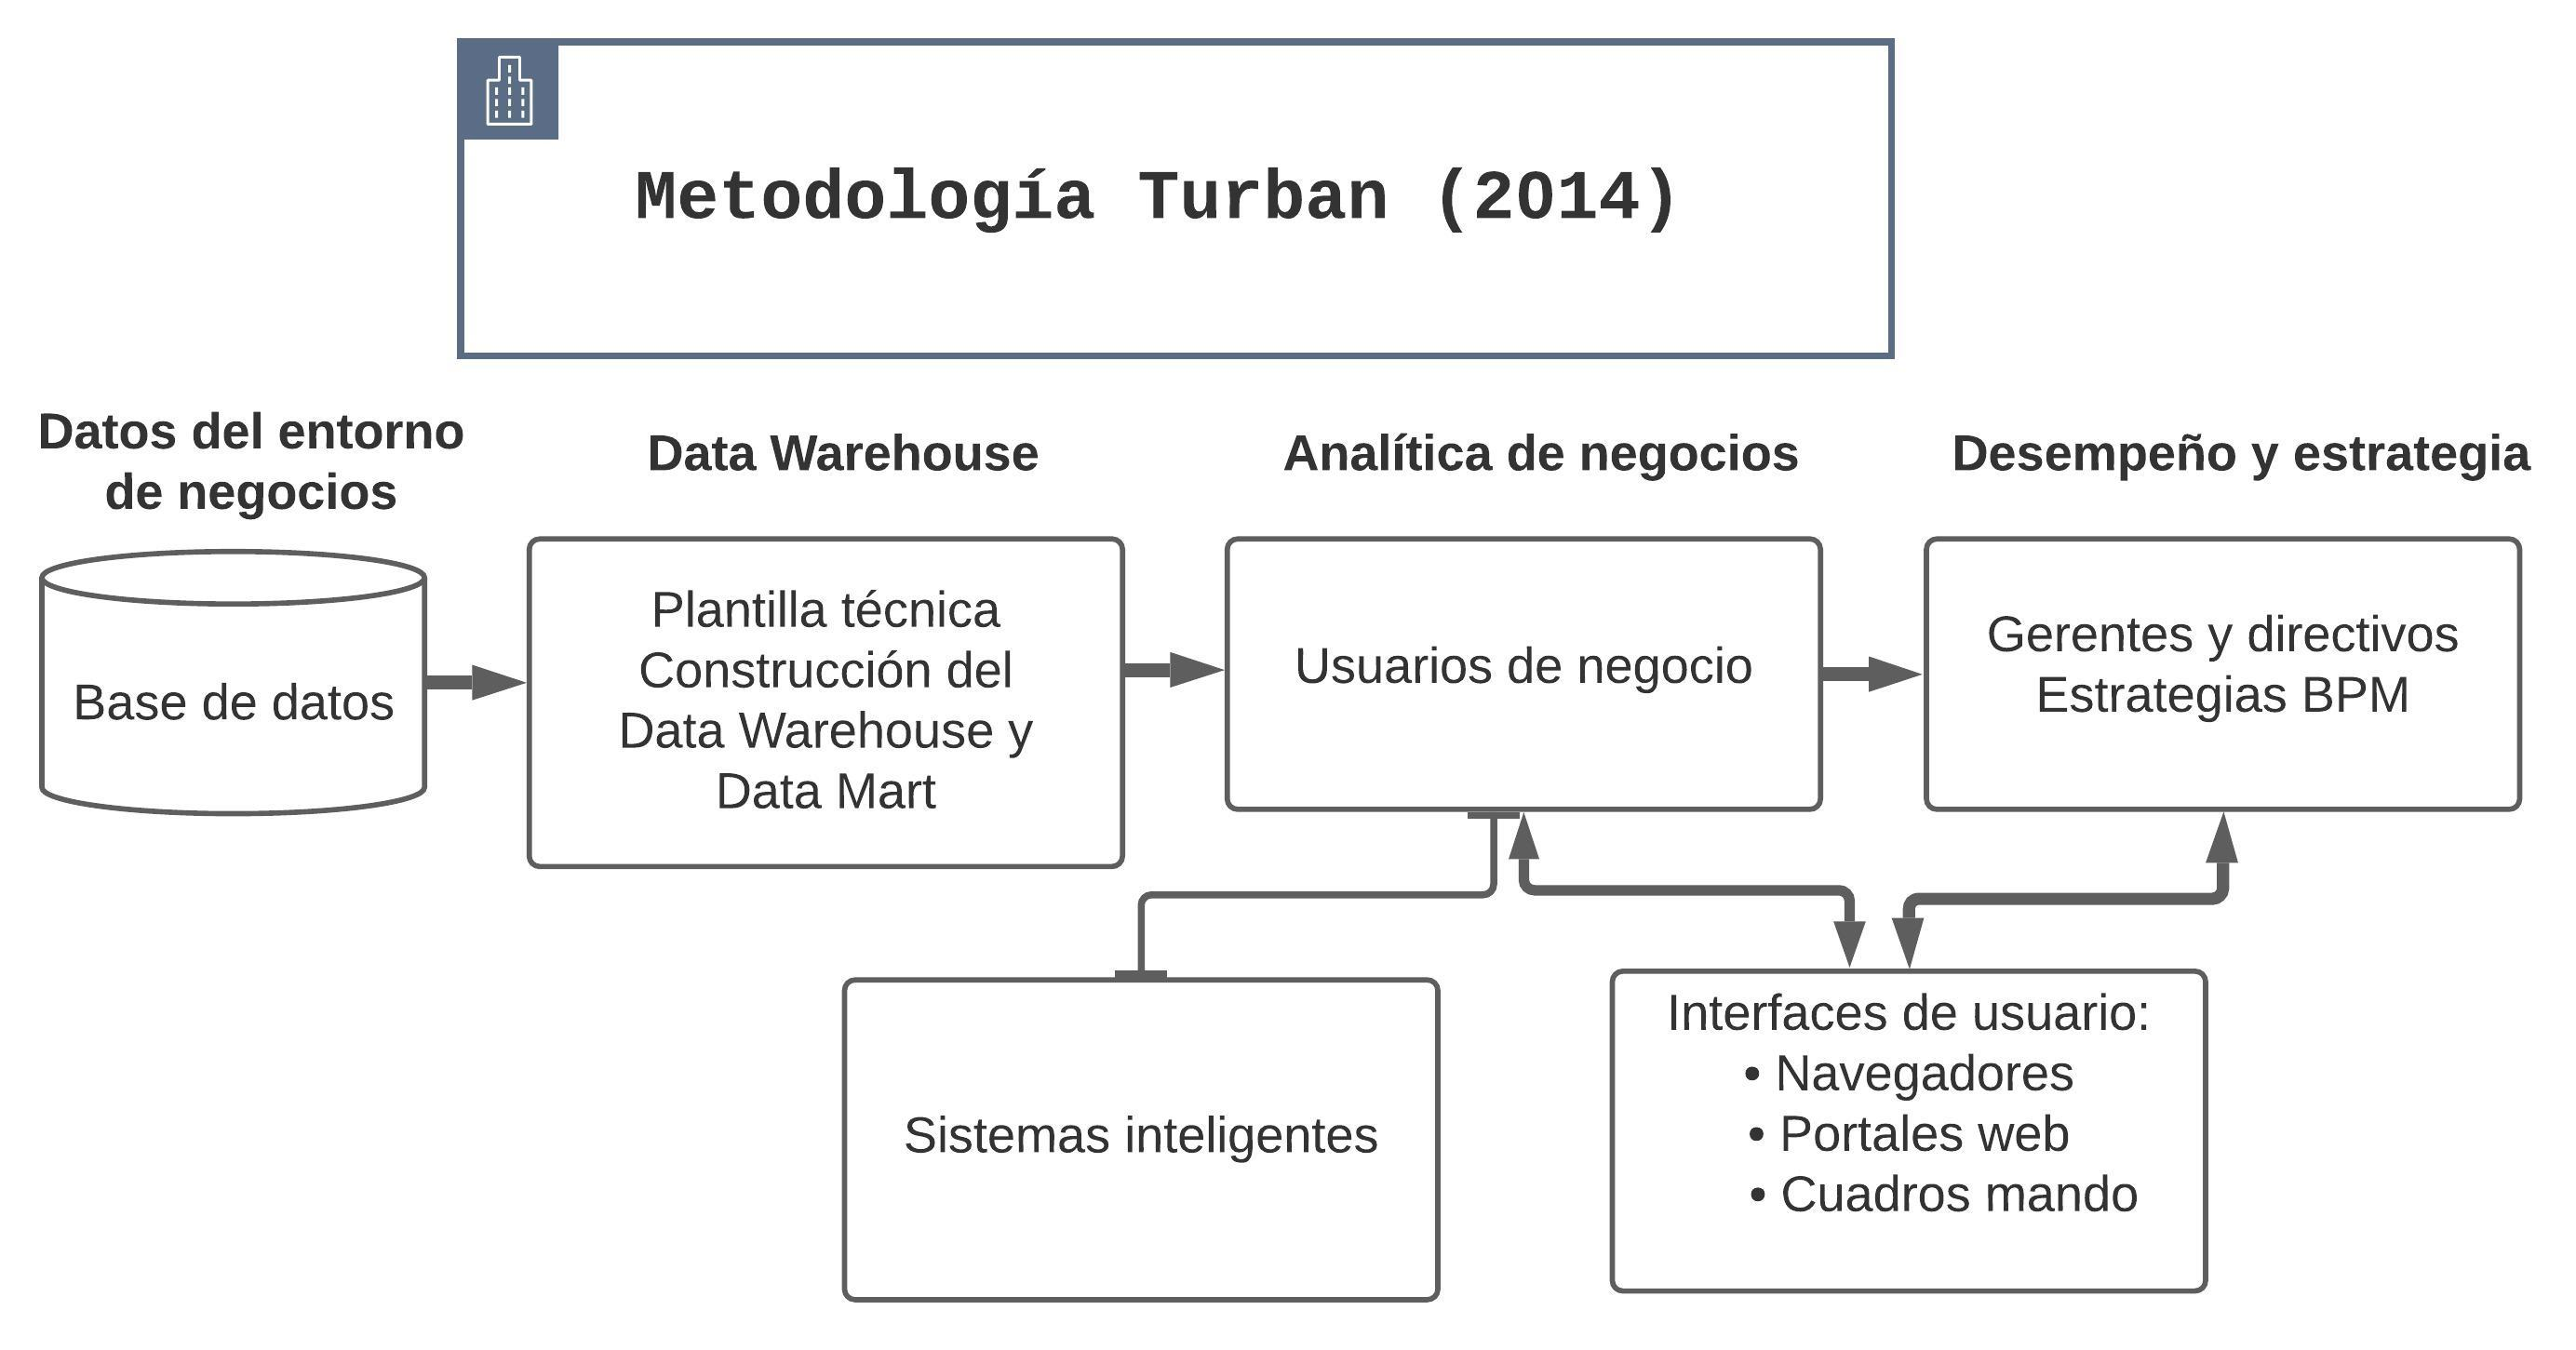
\includegraphics[width=1\linewidth]{Figuras/Met_Turban}
	\caption{Metodología BI - Turban, adaptada del original. [Fuente: Propia]}
	\label{fig: metTurban}
\end{figure}

\begin{description}
\item[1. Deposito de datos - DWH]
Está capa es desarrollada por la plantilla técnica de ingenieros de sistemas e informáticos, para construir los Data Marts (DM) y el Data warehouse (DWH).

\item[2. Analítica de negocios - BA]
Está capa es responsabilidad de los usuarios de negocios que gestionan la información.

\item[3. Administración del rendimiento - BSM]
Está capa es responsabilidad de gerentes y directivos que miden las procesos mediante la metodología BSM y gestionan las interfaces de usuario.

\item[4. Interfaces de usuario - Aplicaciones BI]
Está capa puede ser utilizada por cualquier usuario.\\
\end{description}


\subsubsection{Metodología Laudon}

Laudon (2014) planteo una estructura tecnológica de BI con soporte en las sucesivas ediciones de su edición literaria de sistemas de información mediante seis componentes, a los que se les denomina entornos de BI, como se resumen en la Figura \ref{fig: metLaudon} y se describen, a continuación \cite{lib02}:

\begin{description}
\item[1. Fuentes de datos] 
Son los datos estructurados, no estructurados y semi-estructurados procedentes de numerosas fuentes de datos.

\item[2. Infraestructura de BI]
Son componentes de BI como bases de datos, Data Warehouses, Data Marts y
plataformas de analítica.

\item[3. Herramientas de BA]
Se refiere a herramientas para analizar productos y automatizar informes que respondan a las necesidades de los usuarios, ejecutivos y directivos.

\item[4. Métodos y usuarios gerenciales]
Los directivos y gerentes utilizan el análisis de datos para dar seguimiento a los objetivos estratégicos y gestionar la medición del desempeño.

\item[5. Plataformas de información]
Las plataformas tradicionales son los sistemas de información: MIS, DSS y ESS.

\item[6. Interfaces de usuario]
Las aplicaciones BI son los informes, cuadros de mando y consultas que se deben manipular con dispositivos y tecnologías.
\end{description}

\begin{figure}[h]
	\centering
	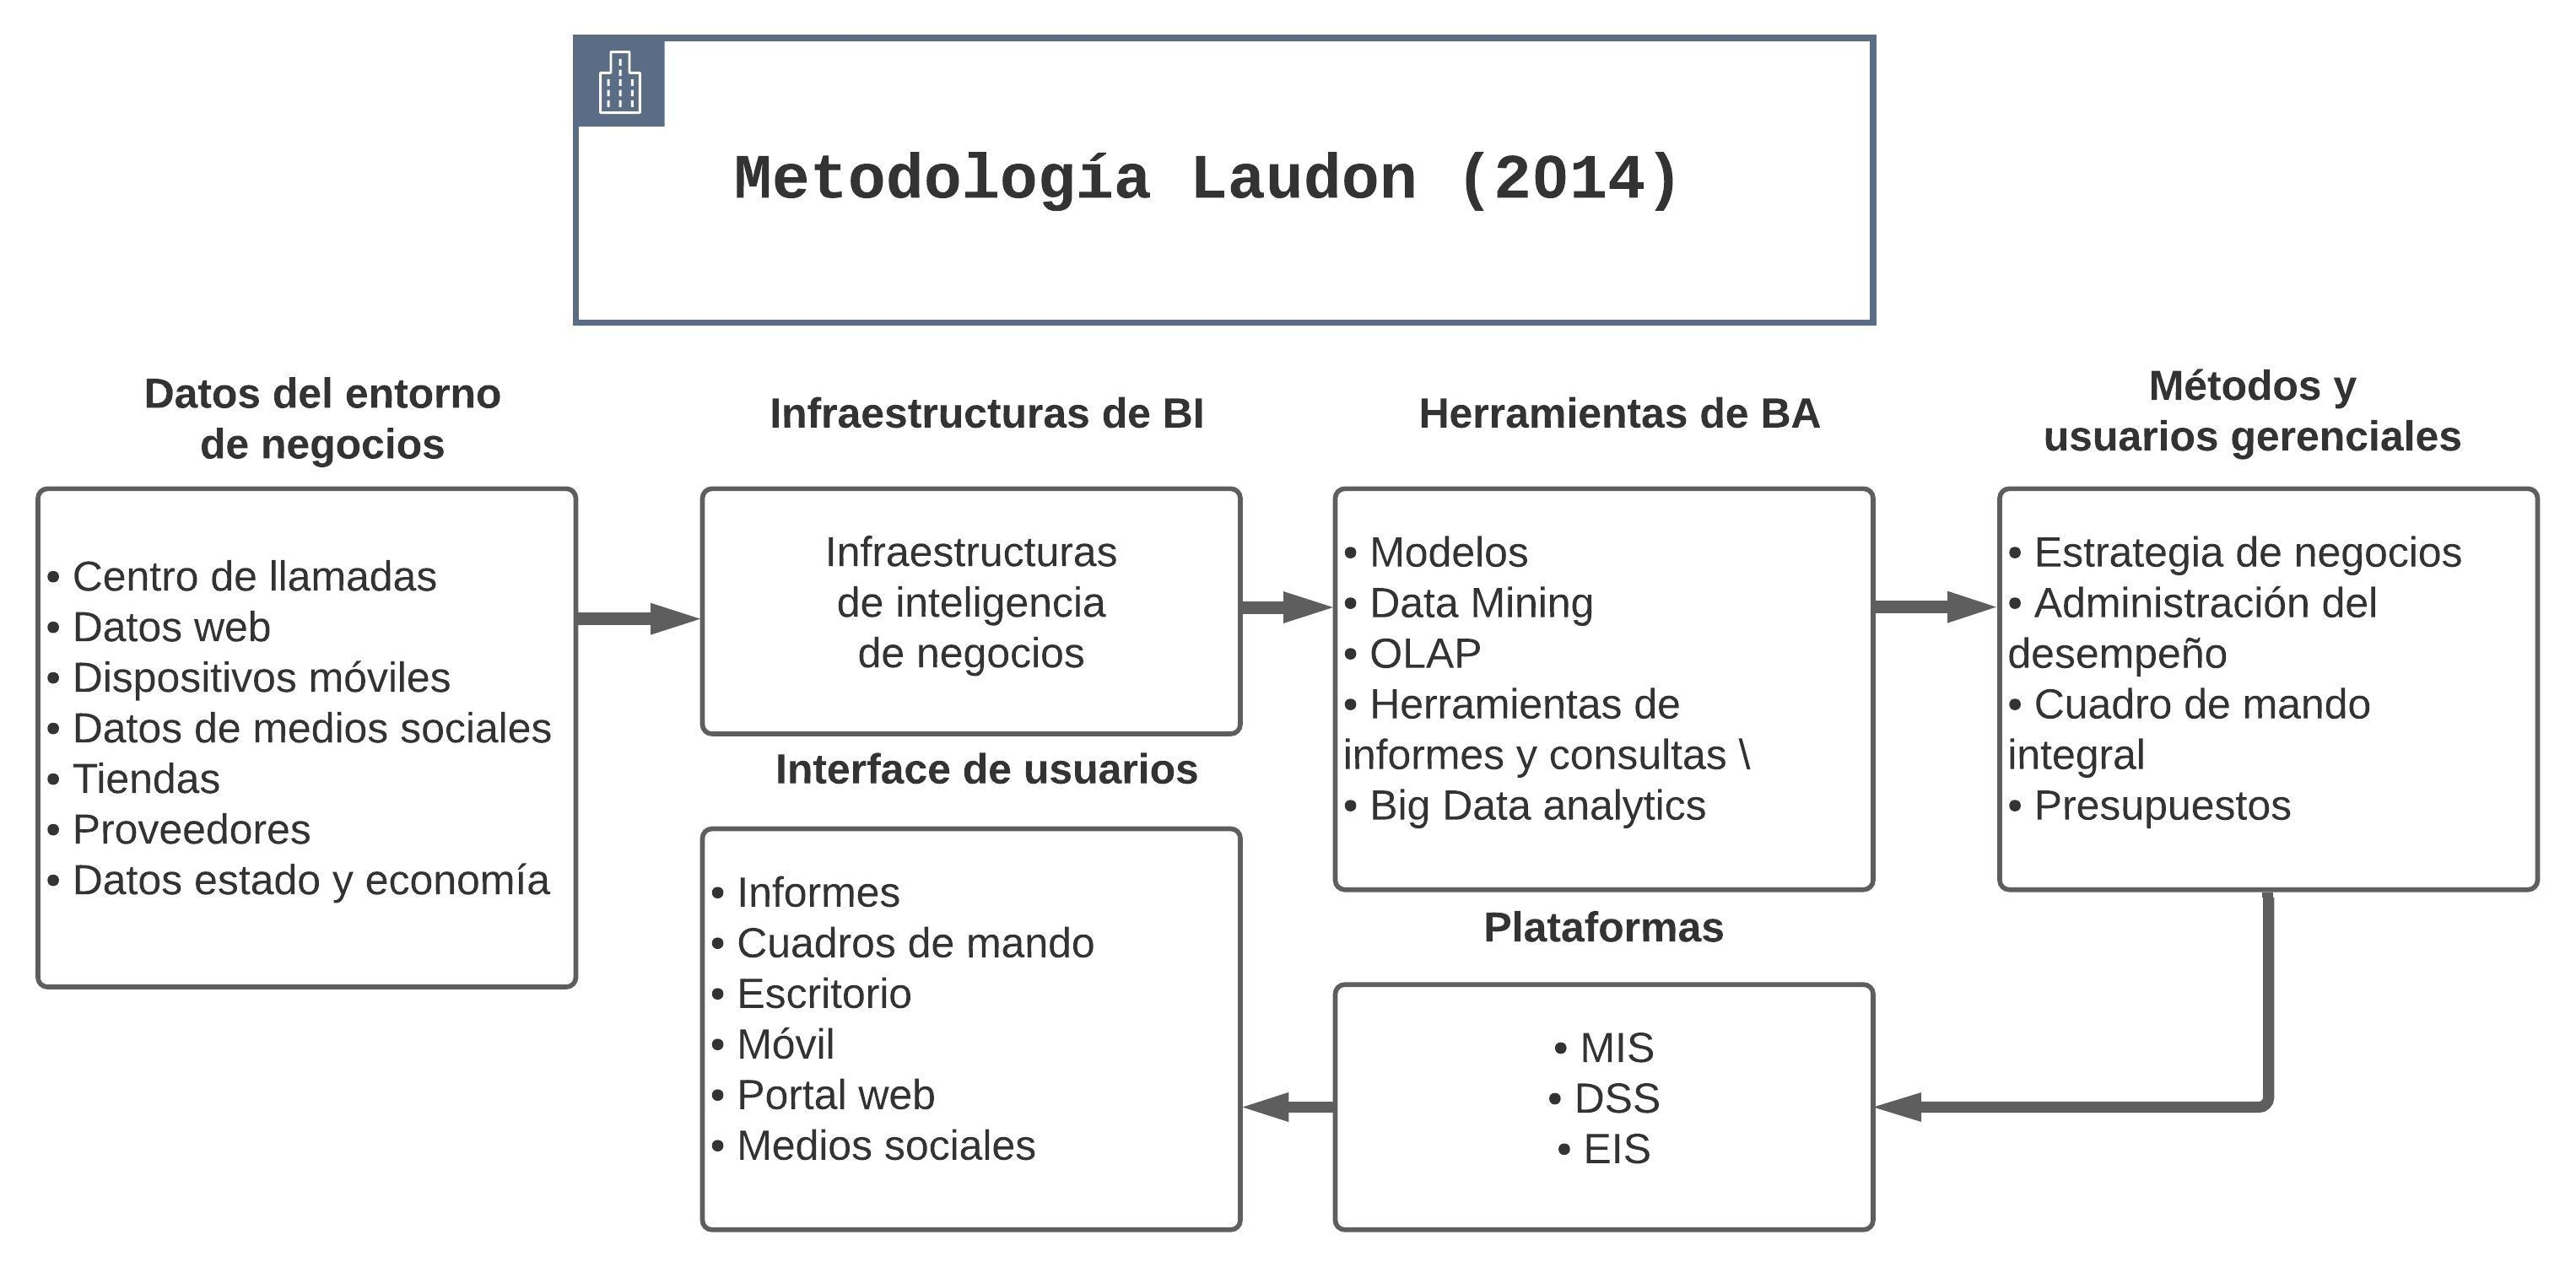
\includegraphics[width=1.08\linewidth]{Figuras/MetLaudon}
	\caption{Metodología BI - Laudon, adaptada del original. [Fuente: Propia]}
	\label{fig: metLaudon}
\end{figure}



\section{Metodología estándar}
Las metodologías modernas son producto de adaptaciones de diferentes procesos de soluciones empresariales, pero cada una depende del planteamiento del problema. En primera instancia, el equipo encargado de la solución BI debe comenzar una implementación de BI con la etapa previa de planificación del proyecto, está define el planteamiento del problema, principalmente los objetivos, justificación y alcance del  proyecto. En segunda instancia, se centra en evaluar la disponibilidad de recursos y requerimientos de personal según la necesidad de información para asignar actividades especificas del proyecto con detalles de tiempo de duración  y frecuencia.\\ 

A continuación, se describe una metodología estándar de BI adaptada de Kimball (2008) muy utilizada en latinoamérica y las componentes que integran su proceso metodológico se pueden resumir en la Figura \ref{fig: metEstandar}.

\begin{figure}[h]
	\centering
	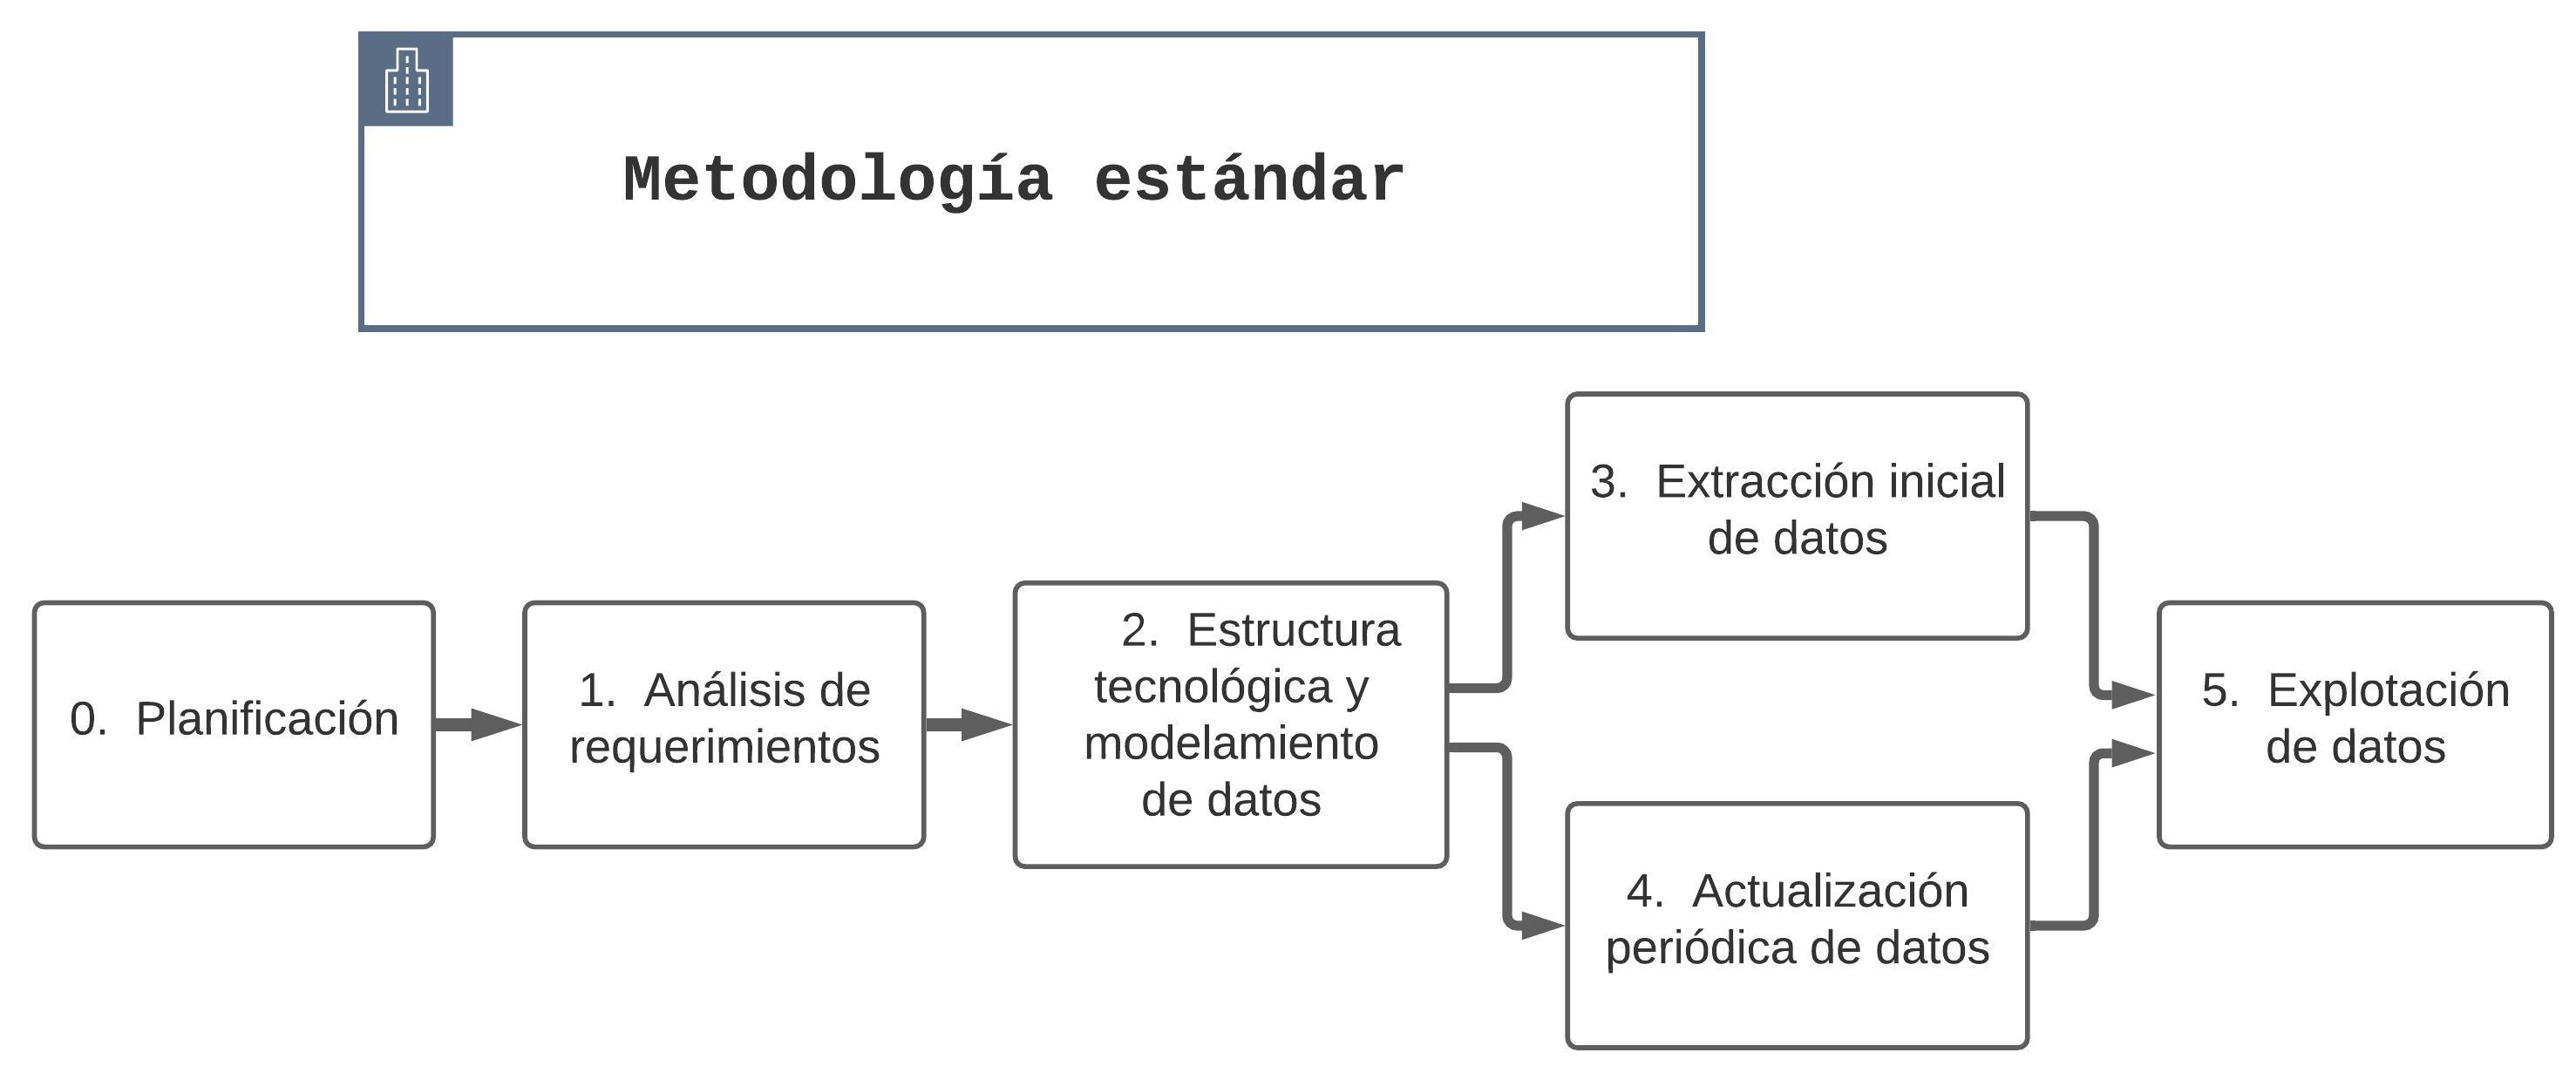
\includegraphics[width=1.08\linewidth]{Figuras/Met_estandar}
	\caption{Metodología estándar adaptada de Kimball (2008). [Fuente: Propia]}
	\label{fig: metEstandar}
\end{figure}


\subsection{Planificación}
Inicialmente, se prioriza desarrollar la etapa preliminar de alinear la estrategia del negocio con las iniciativas BI, las cuales se describen a continuación:
\begin{itemize}
\item[a)] Identificar áreas de oportunidades para aplicar BI
\item[b)] Organizar el personal para afrontar la implementación
\item[c)] Evaluar el impacto de los sistemas operacionales a la solución BI
\item[d)] Seleccionar la tecnología adecuada para su desarrolló
\end{itemize}

En síntesis, este procedimiento tiene como finalidad priorizar el desarrollo incremental utilizando tecnologías para alinear la estrategia de la organización con las iniciativas BI. Esto se puede resumir mediante los elementos base en una estrategia de BI, los cuales se describen en la figura \ref{fig: ElementosBase}.

\begin{figure}[h]
\centering
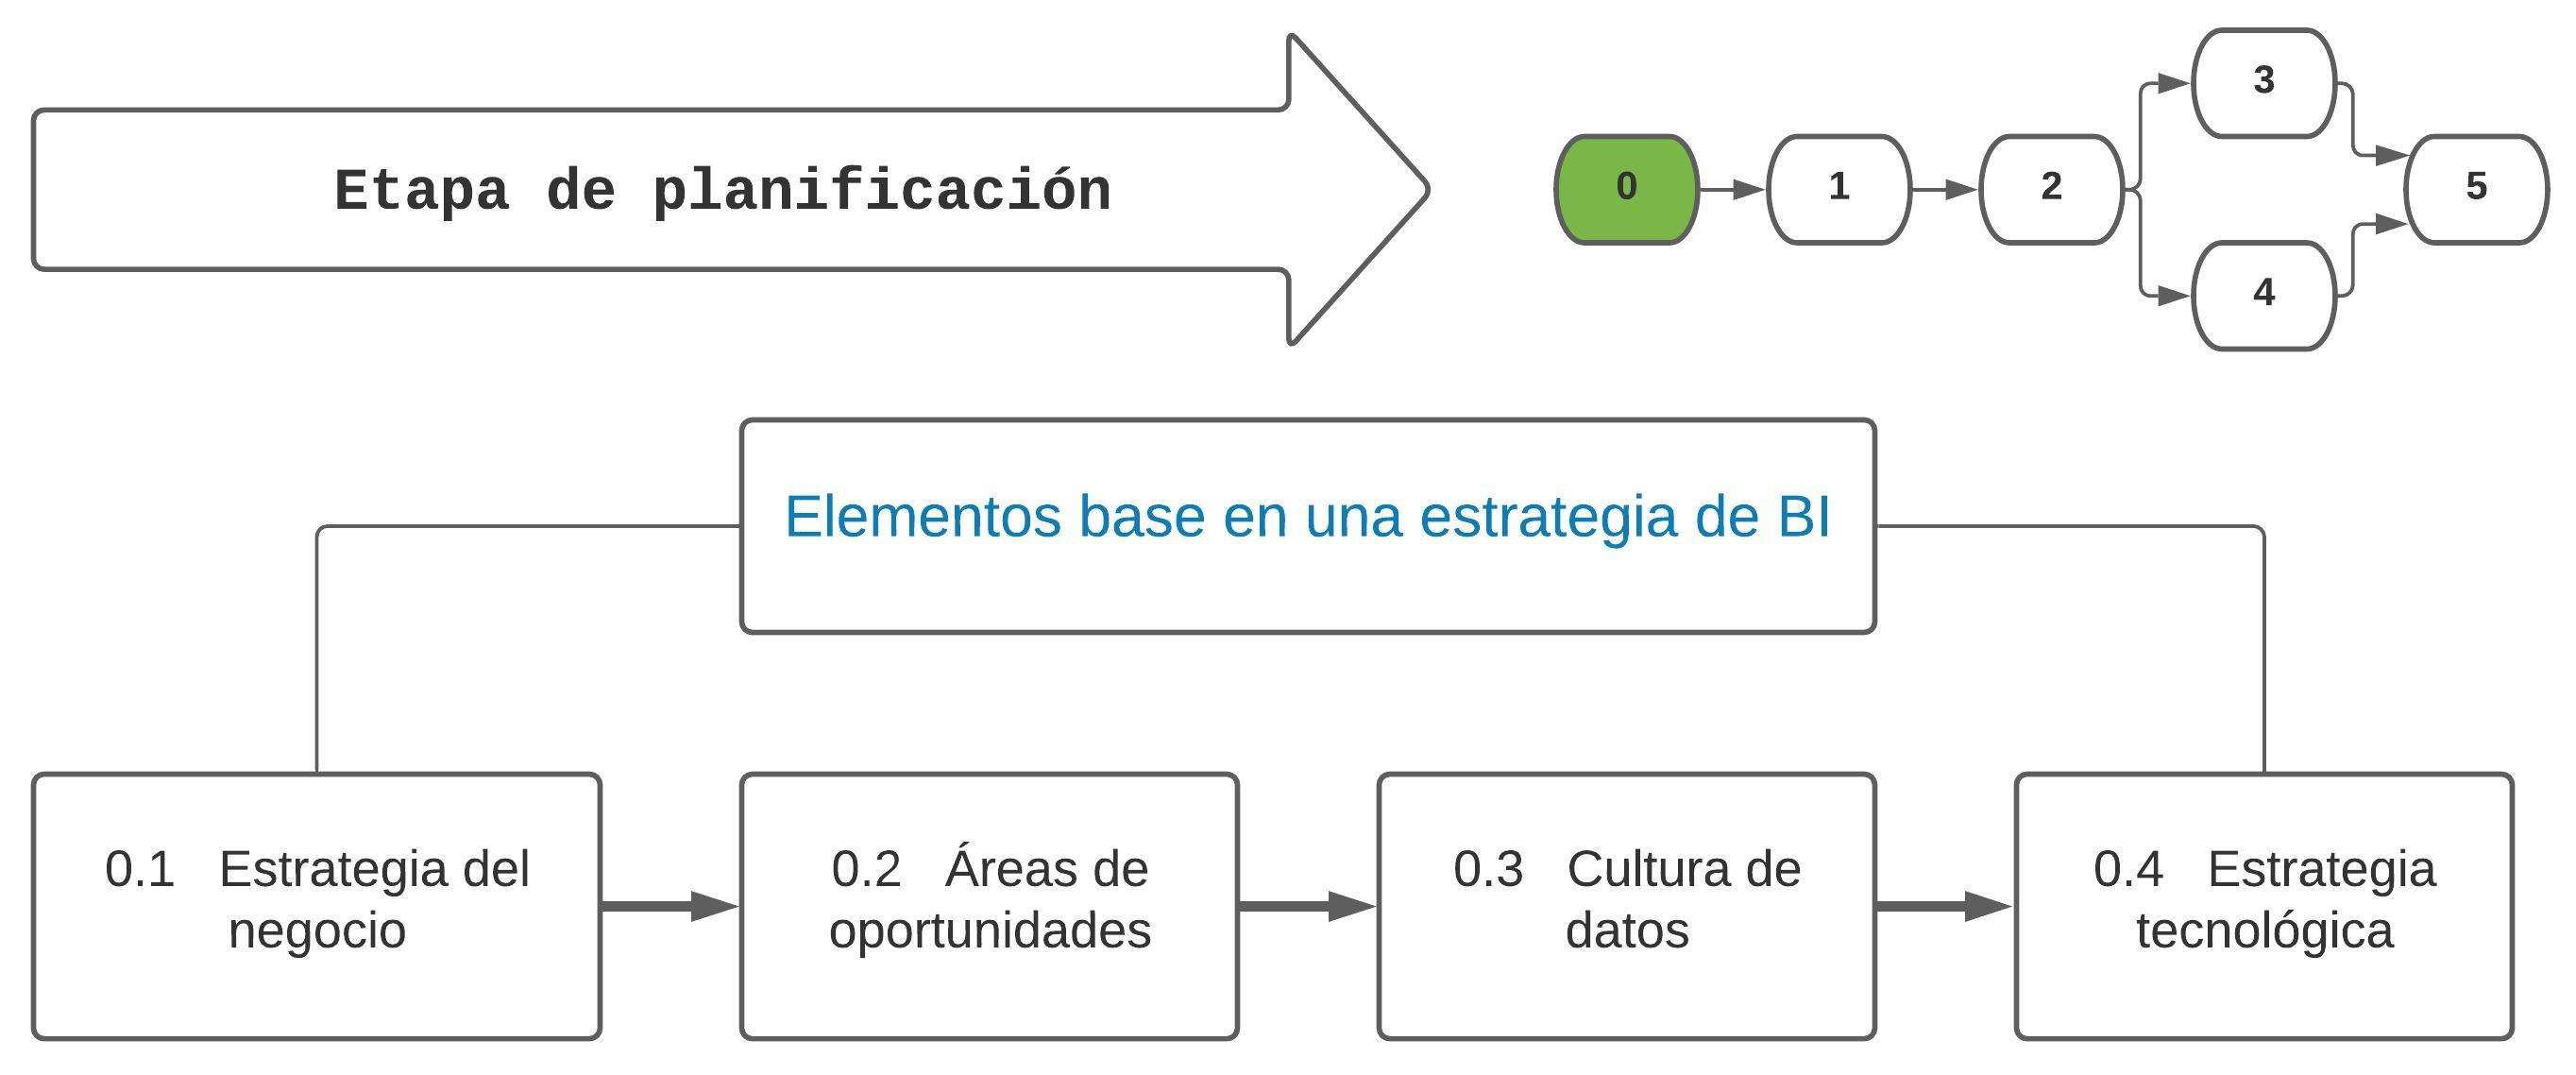
\includegraphics[width=1\linewidth]{Figuras/etapa0}
\caption{Elementos base en una estrategia de BI. [Fuente: Propia]} \label{fig: ElementosBase}	
\end{figure} 

\subsubsection{Estrategia del negocio} 
Una vez alineada la estrategia con las iniciativas BI, se debe realizar el esfuerzo necesario con el uso de la información para apoyar la estrategia del negocio y establecer la contribución que brindan las soluciones empresariales a los negocios.

\subsubsection{Áreas de oportunidades} 
Esencialmente, en esta etapa se identifican las áreas claves de oportunidad para definir las iniciativas BI, este proceso ayuda a desarrollar una cultura de datos y a seleccionar la tecnología idónea.

\subsubsection{Cultura de datos (KH)} 

El esfuerzo con el uso de la información requiere de cambios en la forma de trabajar en las organizaciones para su análisis y desarrollar actividades de manera exitosa. Por tanto, es necesario preparar el personal en aspectos técnicos y funcionales para mejorar las iniciativas. En esta sentido, es importante considerar los aspectos que se describen a continuación:
\begin{multicols}{2}
\begin{itemize}
\item Socializar las expectativas de los usuarios
\item Entrenar el equipo de planificación de recursos de BI
\item Identificar y atenuar problemas de calidad de datos
\item Preparar el cambio tecnológico
\end{itemize}
\end{multicols}
	
Es conclusión, la cultura de datos se refiere a la transferencia de conocimientos, técnicas ó tecnologías (KH, know how) a los usuarios y la preparación del equipo de planificación de recursos.


\subsubsection{Estrategia tecnológica} 
Para desarrollar aplicaciones BI es necesario elegir la tecnología idónea. Por tanto, se considera esencial identificar las necesidades funcionales de los usuarios y ejecutivos en las áreas de oportunidad. Es decir, buscar alternativas tecnológicas idóneas evaluando a los usuarios de la organización en actividades especificas de BI. Esencialmente, esto permite adoptar estándares tecnológicos que garantizan la coherencia en la información, y minimizan costos de implementación, soporte, mantenimiento y formación de usuarios.\\

En consecuencia, es importante identificar los criterios de evaluación en la selección de proveedor para la adopción tecnológica, los cuales se resumen a continuación:

\begin{multicols}{3}
\begin{itemize}
\item Evaluación técnica
\item Evaluación económica
\item Organización y experiencia de proveedor
\item Sistema de oferta
\item Tiempo de respuesta
\item Manejo del volumen de información
\item Facilidad de interfaz
\item Mantenimiento y licenciamiento
\item Solución integrada de la información
\item Portabilidad de la información generada
\item Desarrollo del piloto
\item Tiempo de duración
\item Diseño
\item Producto obtenido
\item Actualización y soporte técnico
\item Garantía 
\item Capacitación
\end{itemize}
\end{multicols}	



\subsection{Análisis de requerimientos} 
En una solución BI, la etapa inicial es determinar los requerimientos de información para dar soporte a la operación y comprender la retroalimentación de la necesidad de información mediante los Star Nets, los cuales describen el diseño lógico de la selección de datos, considerando los aspectos siguientes:
\begin{multicols}{2}
\begin{itemize}
\item[a)] Procesos de actividades
\item[b)] Infraestructura de sistemas operativos
\item[c)] Fuentes de datos
\item[d)] Aplicaciones BI
\end{itemize}
\end{multicols}	

En primera instancia, los usuarios de la organización deberán socializar las necesidades de información con los usuarios responsables de la solución BI para la respectiva evaluación. Este proceso, sintetiza la validación de requerimientos, como se ilustra en la Figura \ref{fig: etapa0}.

\begin{figure}[h]
	\centering
	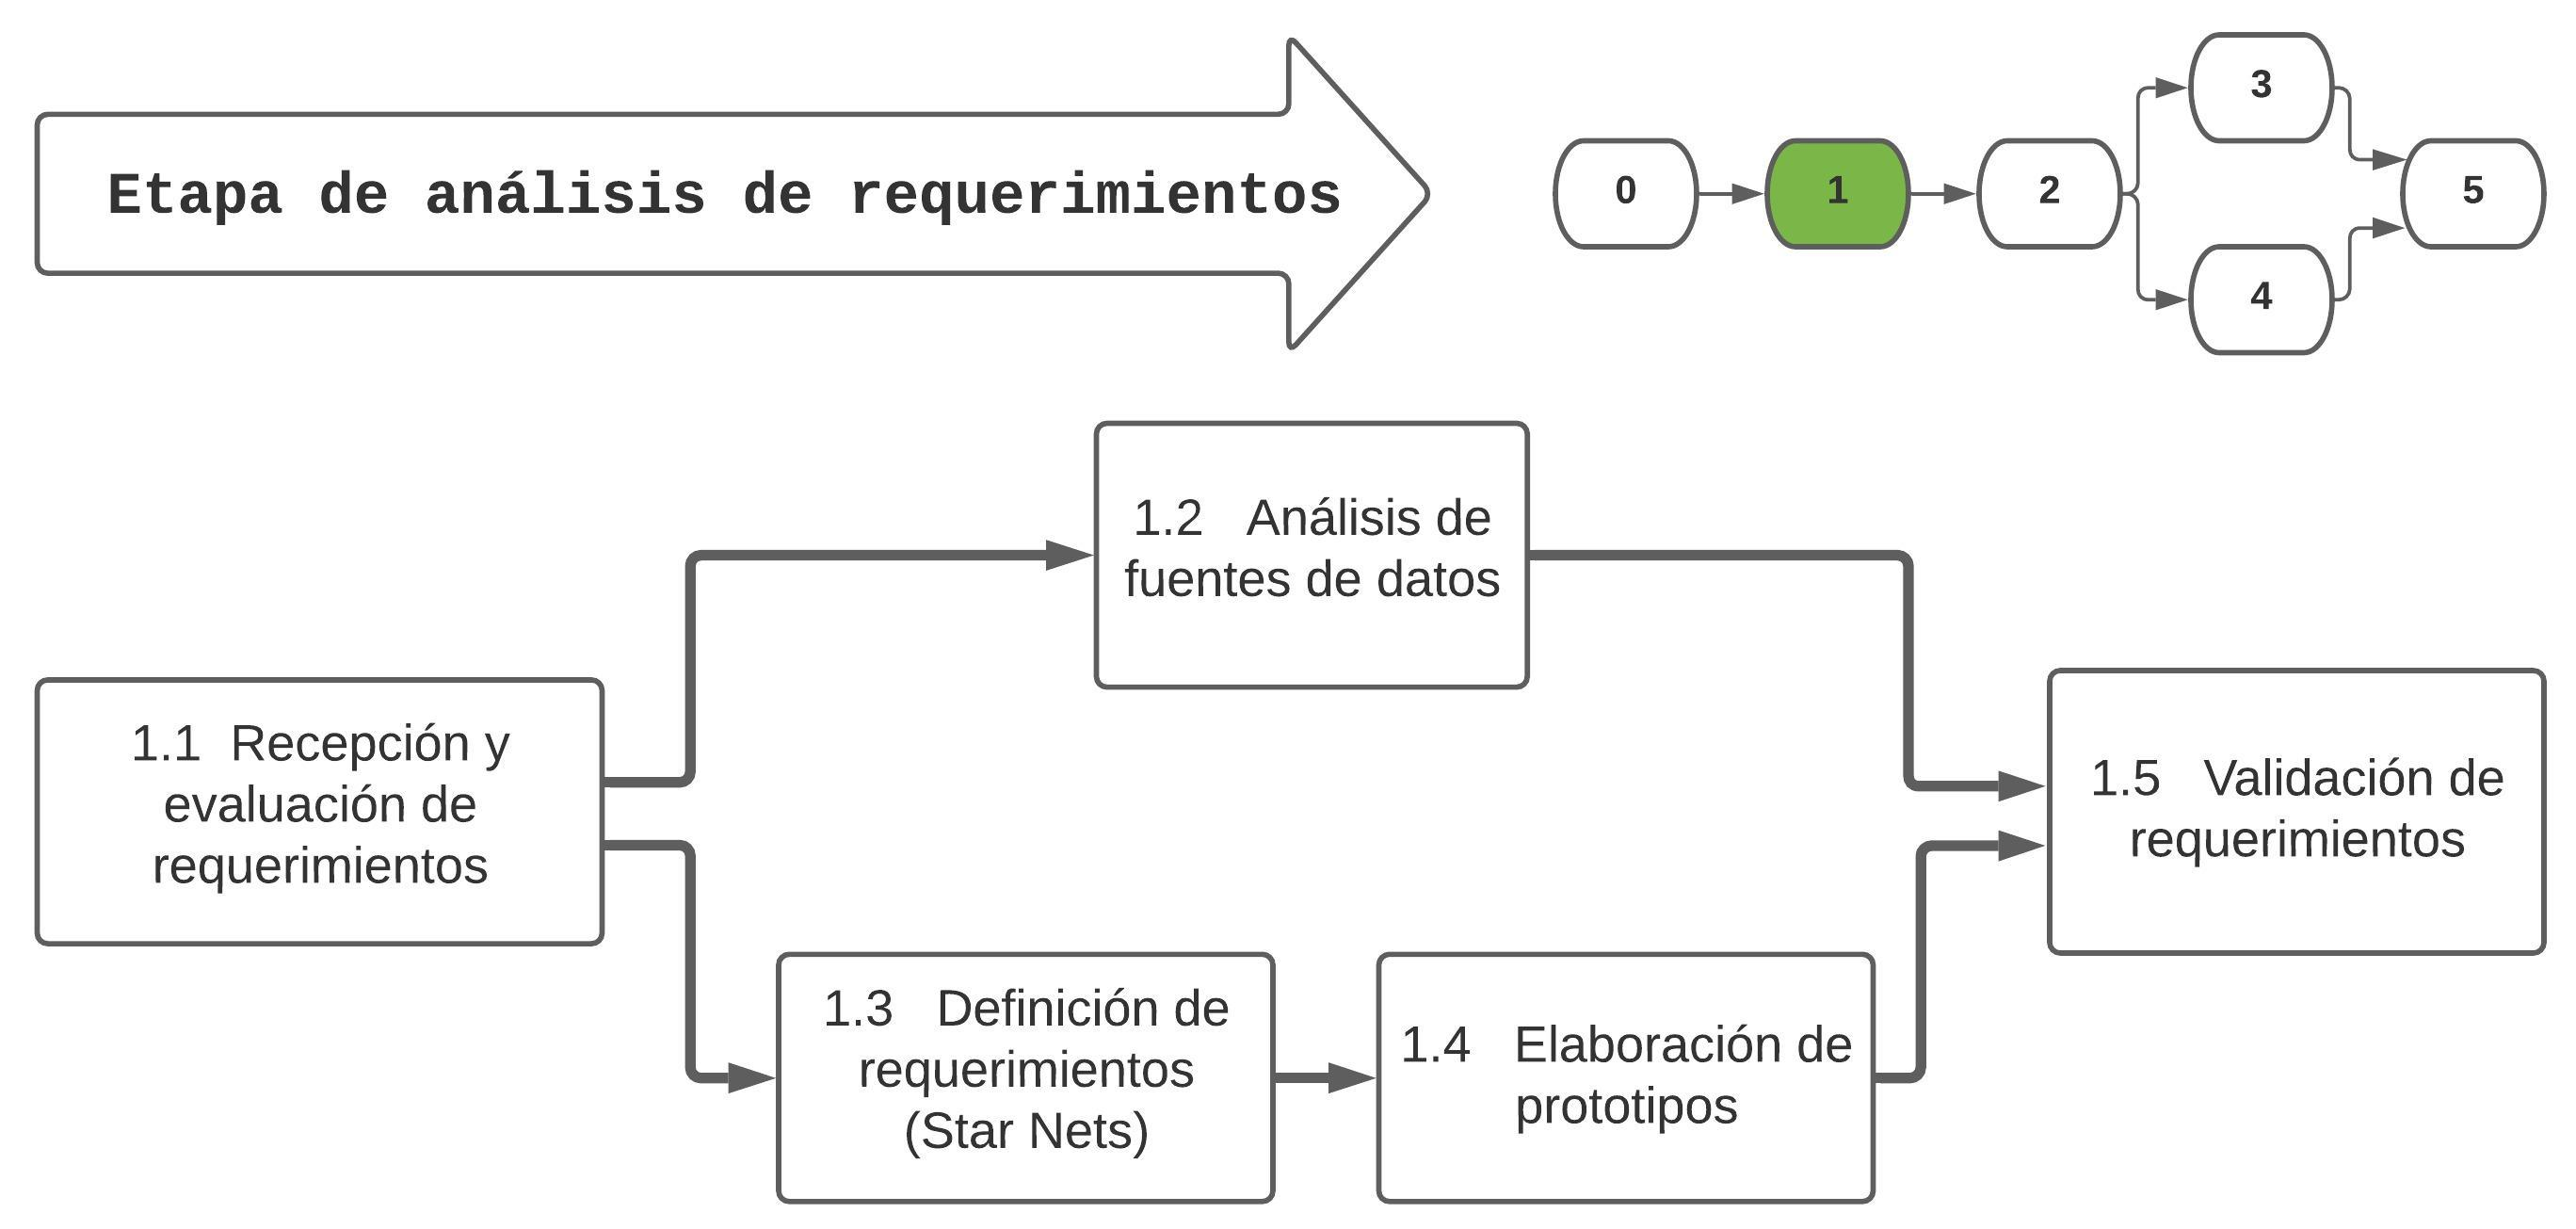
\includegraphics[width=1\linewidth]{Figuras/etapa1}
	\caption{Proceso metodológico del análisis de requerimientos. [Fuente: Propia]}
	\label{fig: etapa0}
\end{figure}

\begin{wrapfigure}{c}{0.47\linewidth}
\scalebox{1}{
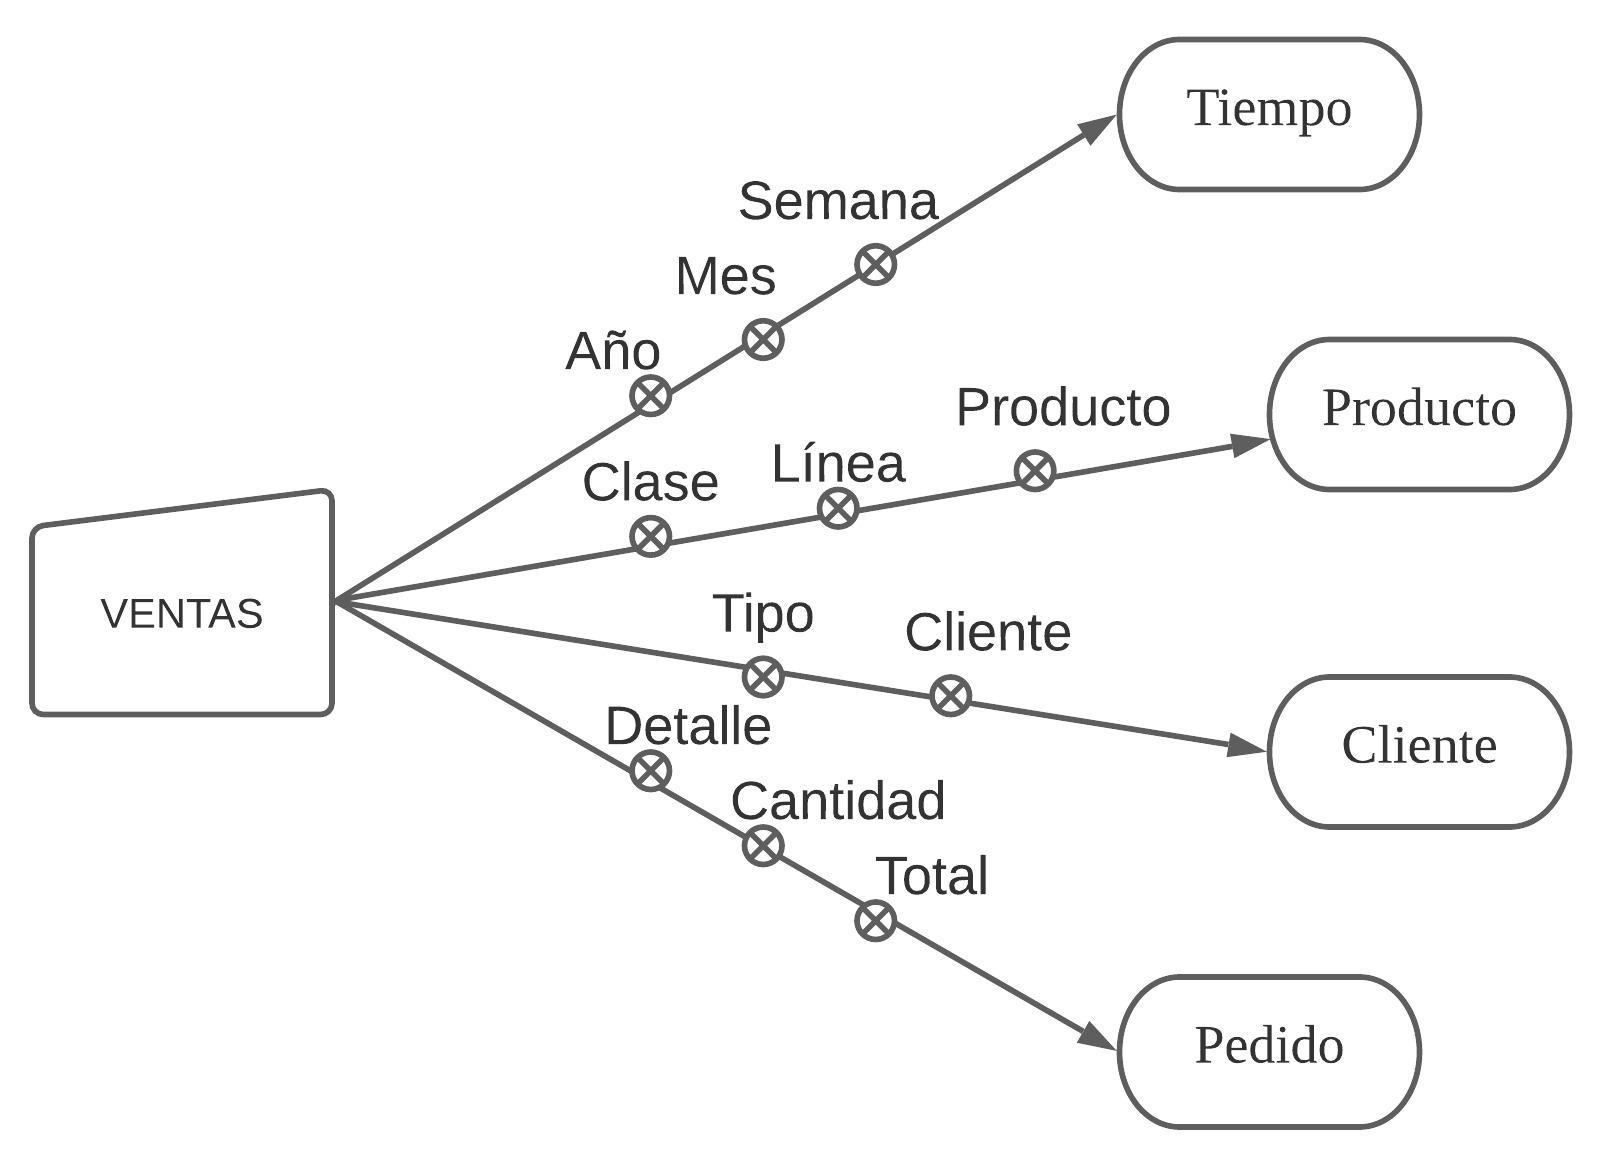
\includegraphics[width=1.1\linewidth]{Figuras/starNet} }
\caption{Ejemplo de Star Nets de la métrica de ventas. [Fuente: Propia]}
\label{fig: starnet}
\end{wrapfigure}

En segunda instancia, se analizan las fuentes de datos disponibles para definir los requerimientos y diseñar los 'Star Nets' que identifican todas las variables y los macrodatos que describen las mediciones requeridas o métricas, donde las variables son los criterios basados en la necesidad de información para la elaboración de prototipos. Esta idea, se puede esquematizar con un diagrama funcional que consolida las variables y métricas, por ejemplo, el Star Nets particular del modelo de gestión de ventas en el Cuadro \ref{Cuadro: ModelosG} que se muestra en la Figura \ref{fig: starnet}.



\subsection{Estructura tecnológica y modelado dimensional} 
Un modelo de base de datos determina la estructura lógica de una base de datos, y además, determina la forma de almacenar y manipular los datos. En perspectiva, se describe el modelamiento dimensional del proceso metodológico basado en la estructura tecnológica estándar, la cual se resume en la Figura \ref{fig: etapa2}.

\begin{figure}[h]
	\centering
	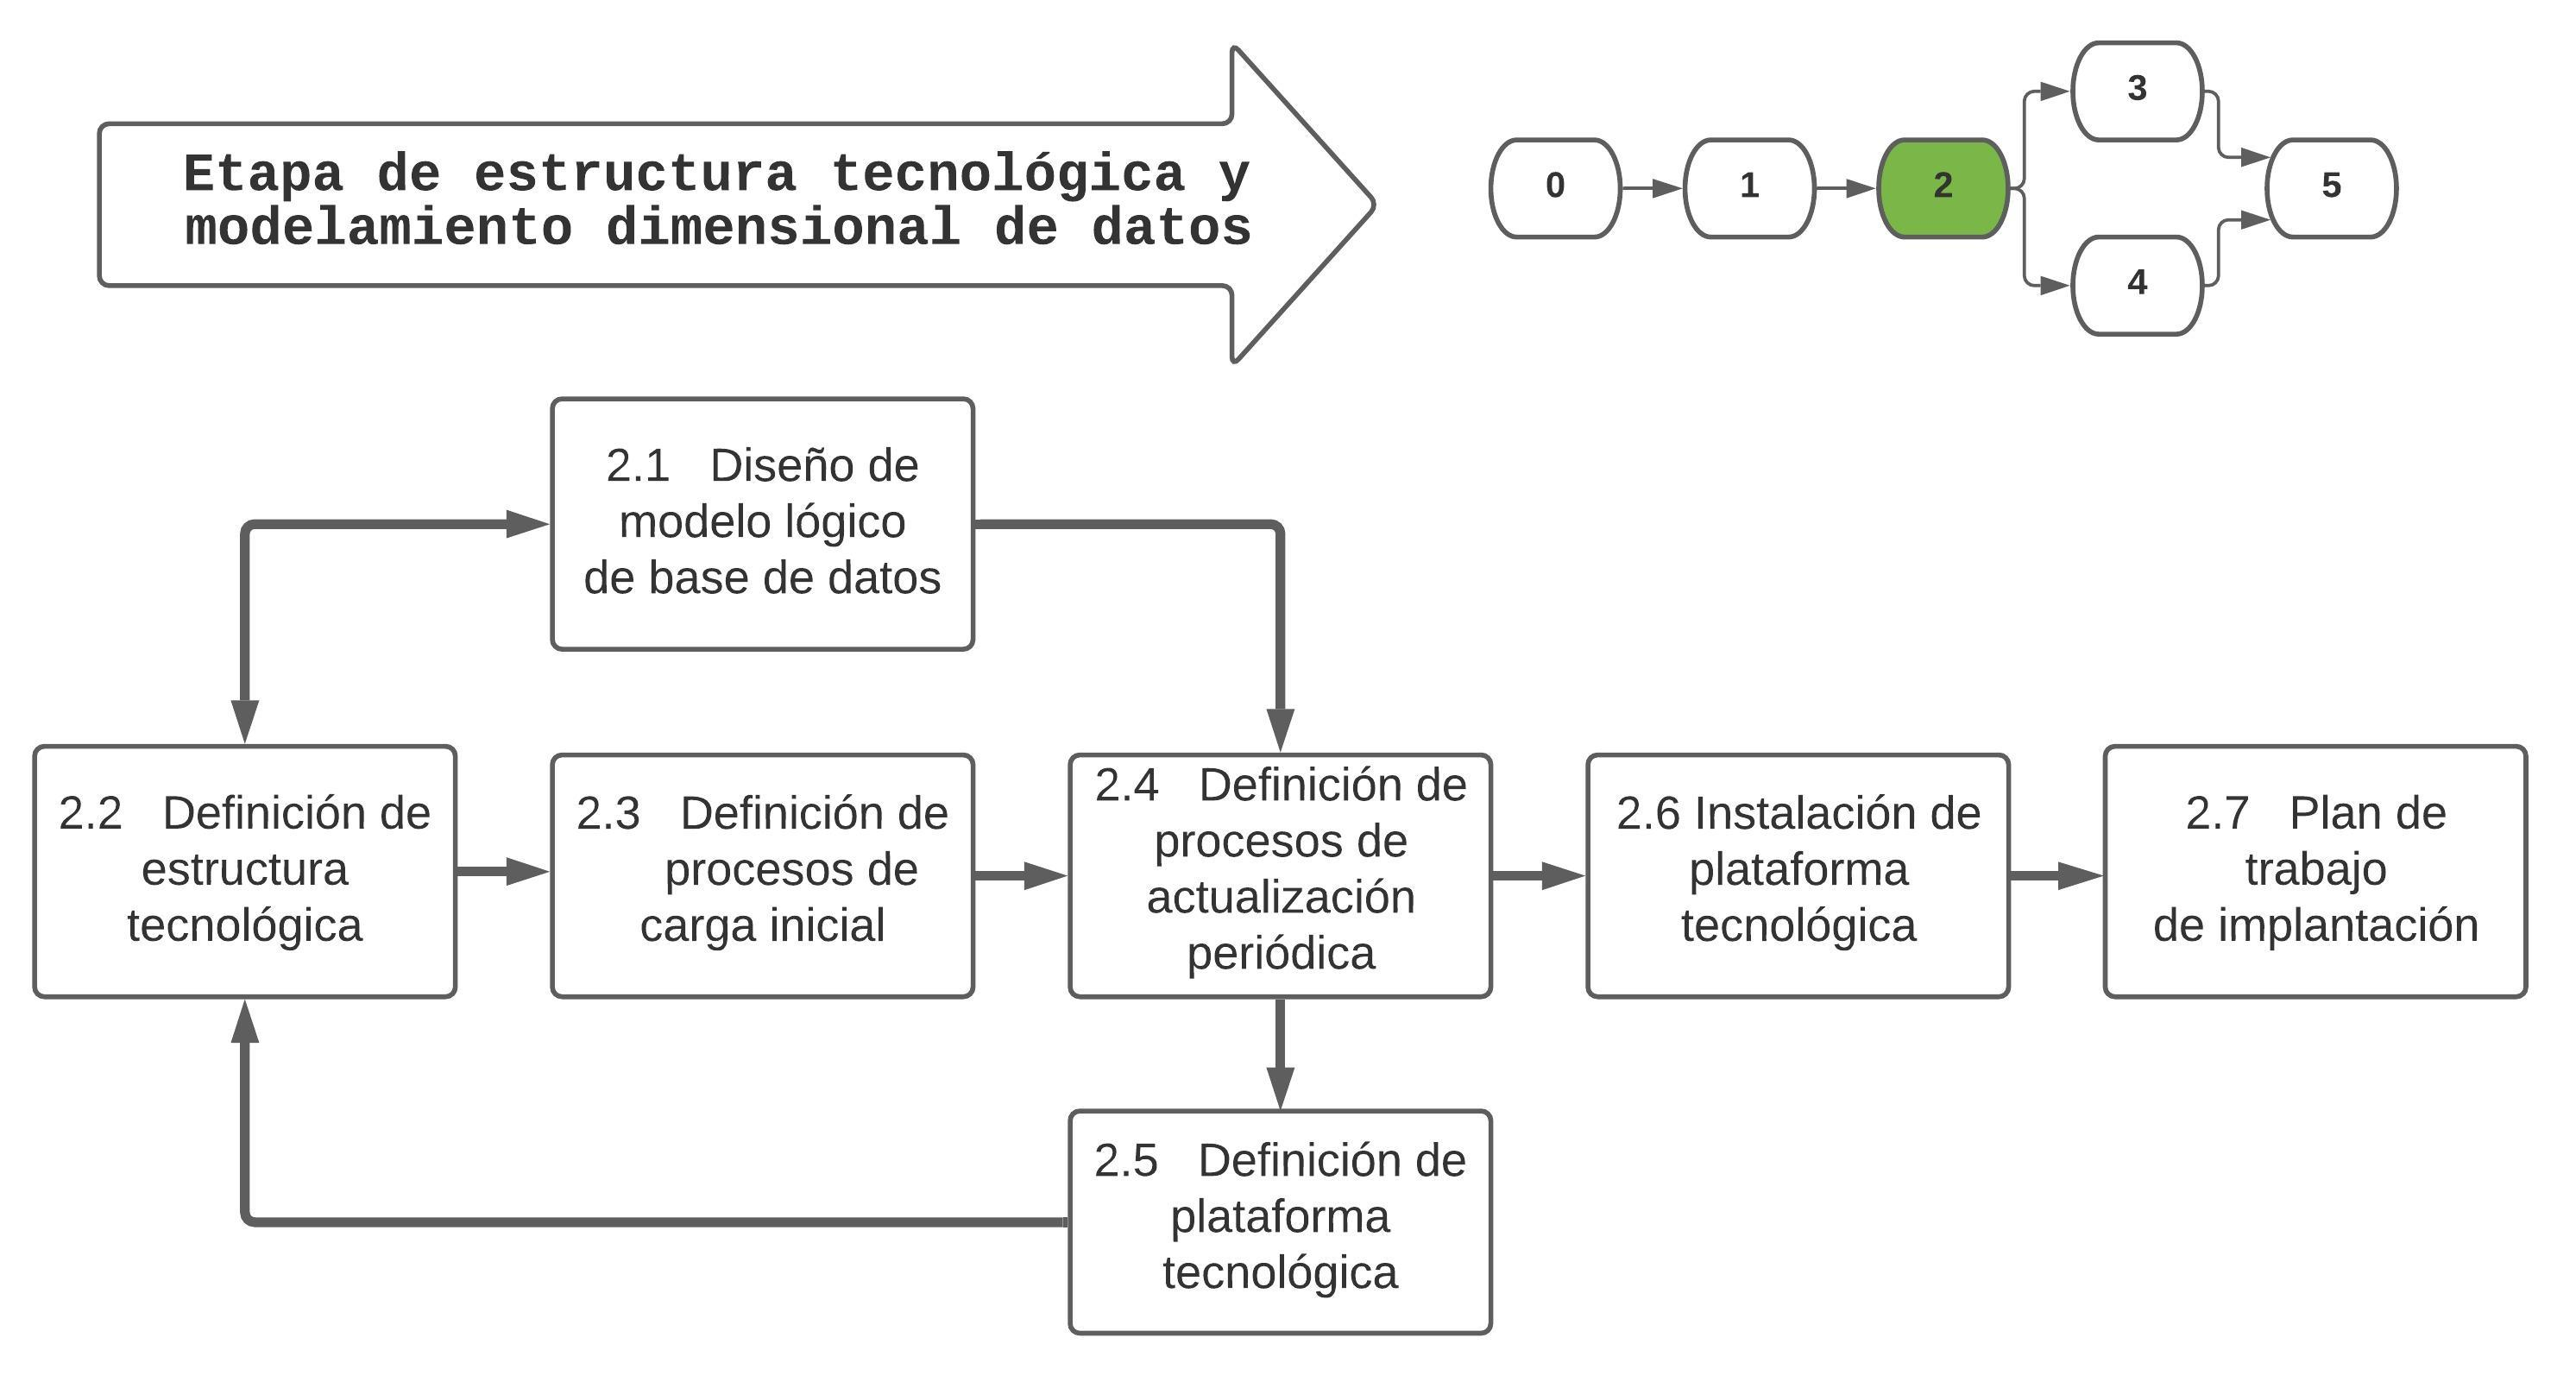
\includegraphics[width=1\linewidth]{Figuras/etapa2}
	\caption{Proceso metodológico del modelamiento dimensional. [Fuente: Propia]}
	\label{fig: etapa2}
\end{figure}

\subsubsection{Plataforma tecnológica}
Ciertamente, la estructura tecnológica estándar es utilizada para desarrollar el proceso del modelo de datos. En resumen, luego de realizar el análisis de requerimientos, se comienza un proceso más técnico como definir los procesos de carga y finalmente, instalar una plataforma tecnológica. Esta etapa, debe considerar las fuentes de datos operacionales, especificaciones del servidor y adquisición de la licencia de la base de datos del deposito, instancias de procesos de cargas periódicas y aplicaciones BI.


\subsubsection{Modelado dimensional (DMo)}
El modelado dimensional (DMo, Dimensional modeling) Es una técnica de diseño lógico con la finalidad de presentar la información en una estructura estándar que permite acceso de alto desempeño a los datos. Particularmente, el esquema estrella separa los datos del proceso de negocios en tablas de hechos y de dimensiones. Normalmente, el modelamiento dimensional está basado en un modelo denominado <<modelo estrella>>, además de una variante del esquema estrella denominado <<copo de nieve>>.\\

El diseño del modelo estrella se compone por una tabla central o de hechos, que contiene las métricas del negocio, y en su entorno, se acoplan las tablas dimensionales cuyos atributos son los criterios basados en la necesidad de información. Esté diseño lógico se puede ilustrar con el ejemplo del modelo de gestión de ventas en el Cuadro \ref{Cuadro: ModelosG} que se muestra en la Figura \ref{fig: starModel}.

\begin{figure}[h]
	\centering
	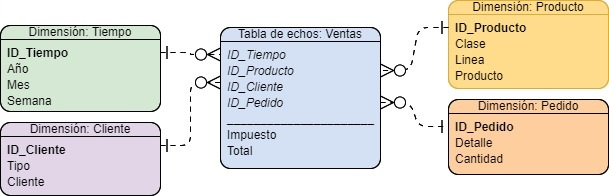
\includegraphics[width=1\linewidth]{Figuras/starModel}
	\caption{Ejemplo del modelo estrella de ventas. [Fuente: Propia]}
	\label{fig: starModel}
\end{figure}

La utilidad del modelo estrella en el modelamiento dimensional de datos se puede apreciar en base a sus características, de las cuales se resaltan las siguientes:

\begin{multicols}{2}
\begin{itemize}

\item Las tablas dimensionales contienen una clave propia (clave primaria) en cada una de ellas. Dicha clave es autogenerada para garantizar atributos de filtración.

\item La clave primaria de la tabla de hechos es la combinación de las claves de las tablas dimensionales para mantener una integridad referencial.

\end{itemize}
\end{multicols}	


\subsubsection{Normalización de los datos}
El modelo de entidad-relación requiere de normalizar los datos con el objeto de minimizar la redundancia. La normalización, consiste en aplicar reglas en el proceso de transformación al modelo relacional. Por otra parte, a partir de un modelo desnormalizado la metodología estándar (Kimball) busca generar respuestas a las consultas de manera dinámica. En este sentido, la idea intuitiva de un modelo estrella es el recorrido inverso al de un sistema basado en entidad-relación.\\

Valga la comparación, la metodología de Inmon se basa en conceptos de bases de datos relacionales (Inmon 02, Imhoff \& Galemmo 03). Su metodología de implementación es la habitual para diseñar modelos de gestión de la información y es contrario a la metodología de Kimball, en el sentido que esta basada en el modelado dimensional.\\


\subsection{Procesos ETL}
En está etapa se considera el diseño y desarrolló de los procesos ETL (Extract, Transform and Load) de extracción, transformación y carga necesarios para la alimentación inicial y periódica del modelo de datos.\\

Prácticamente, la extracción consiste en identificar y capturar los datos de fuentes, mientra que la transformación aplica un conjunto de reglas y tratamientos de limpieza para transformar los datos. Finalmente, se realiza la carga de datos al modelo. Este proceso se divide en extracción inicial y carga periódica de los datos.\\

\subsection{Extracción inicial}

permite extraer información de producción inicial a los Data Mart de diferentes fuentes de datos que requieren ser procesadas, según los procesos de carga descritos en la etapa del modelamiento de datos. Este proceso metodológico es una adaptación de Kimball y Ross (2002) y se resume en la Figura \ref{fig: etapa3}.

\begin{figure}[h]
	\centering
	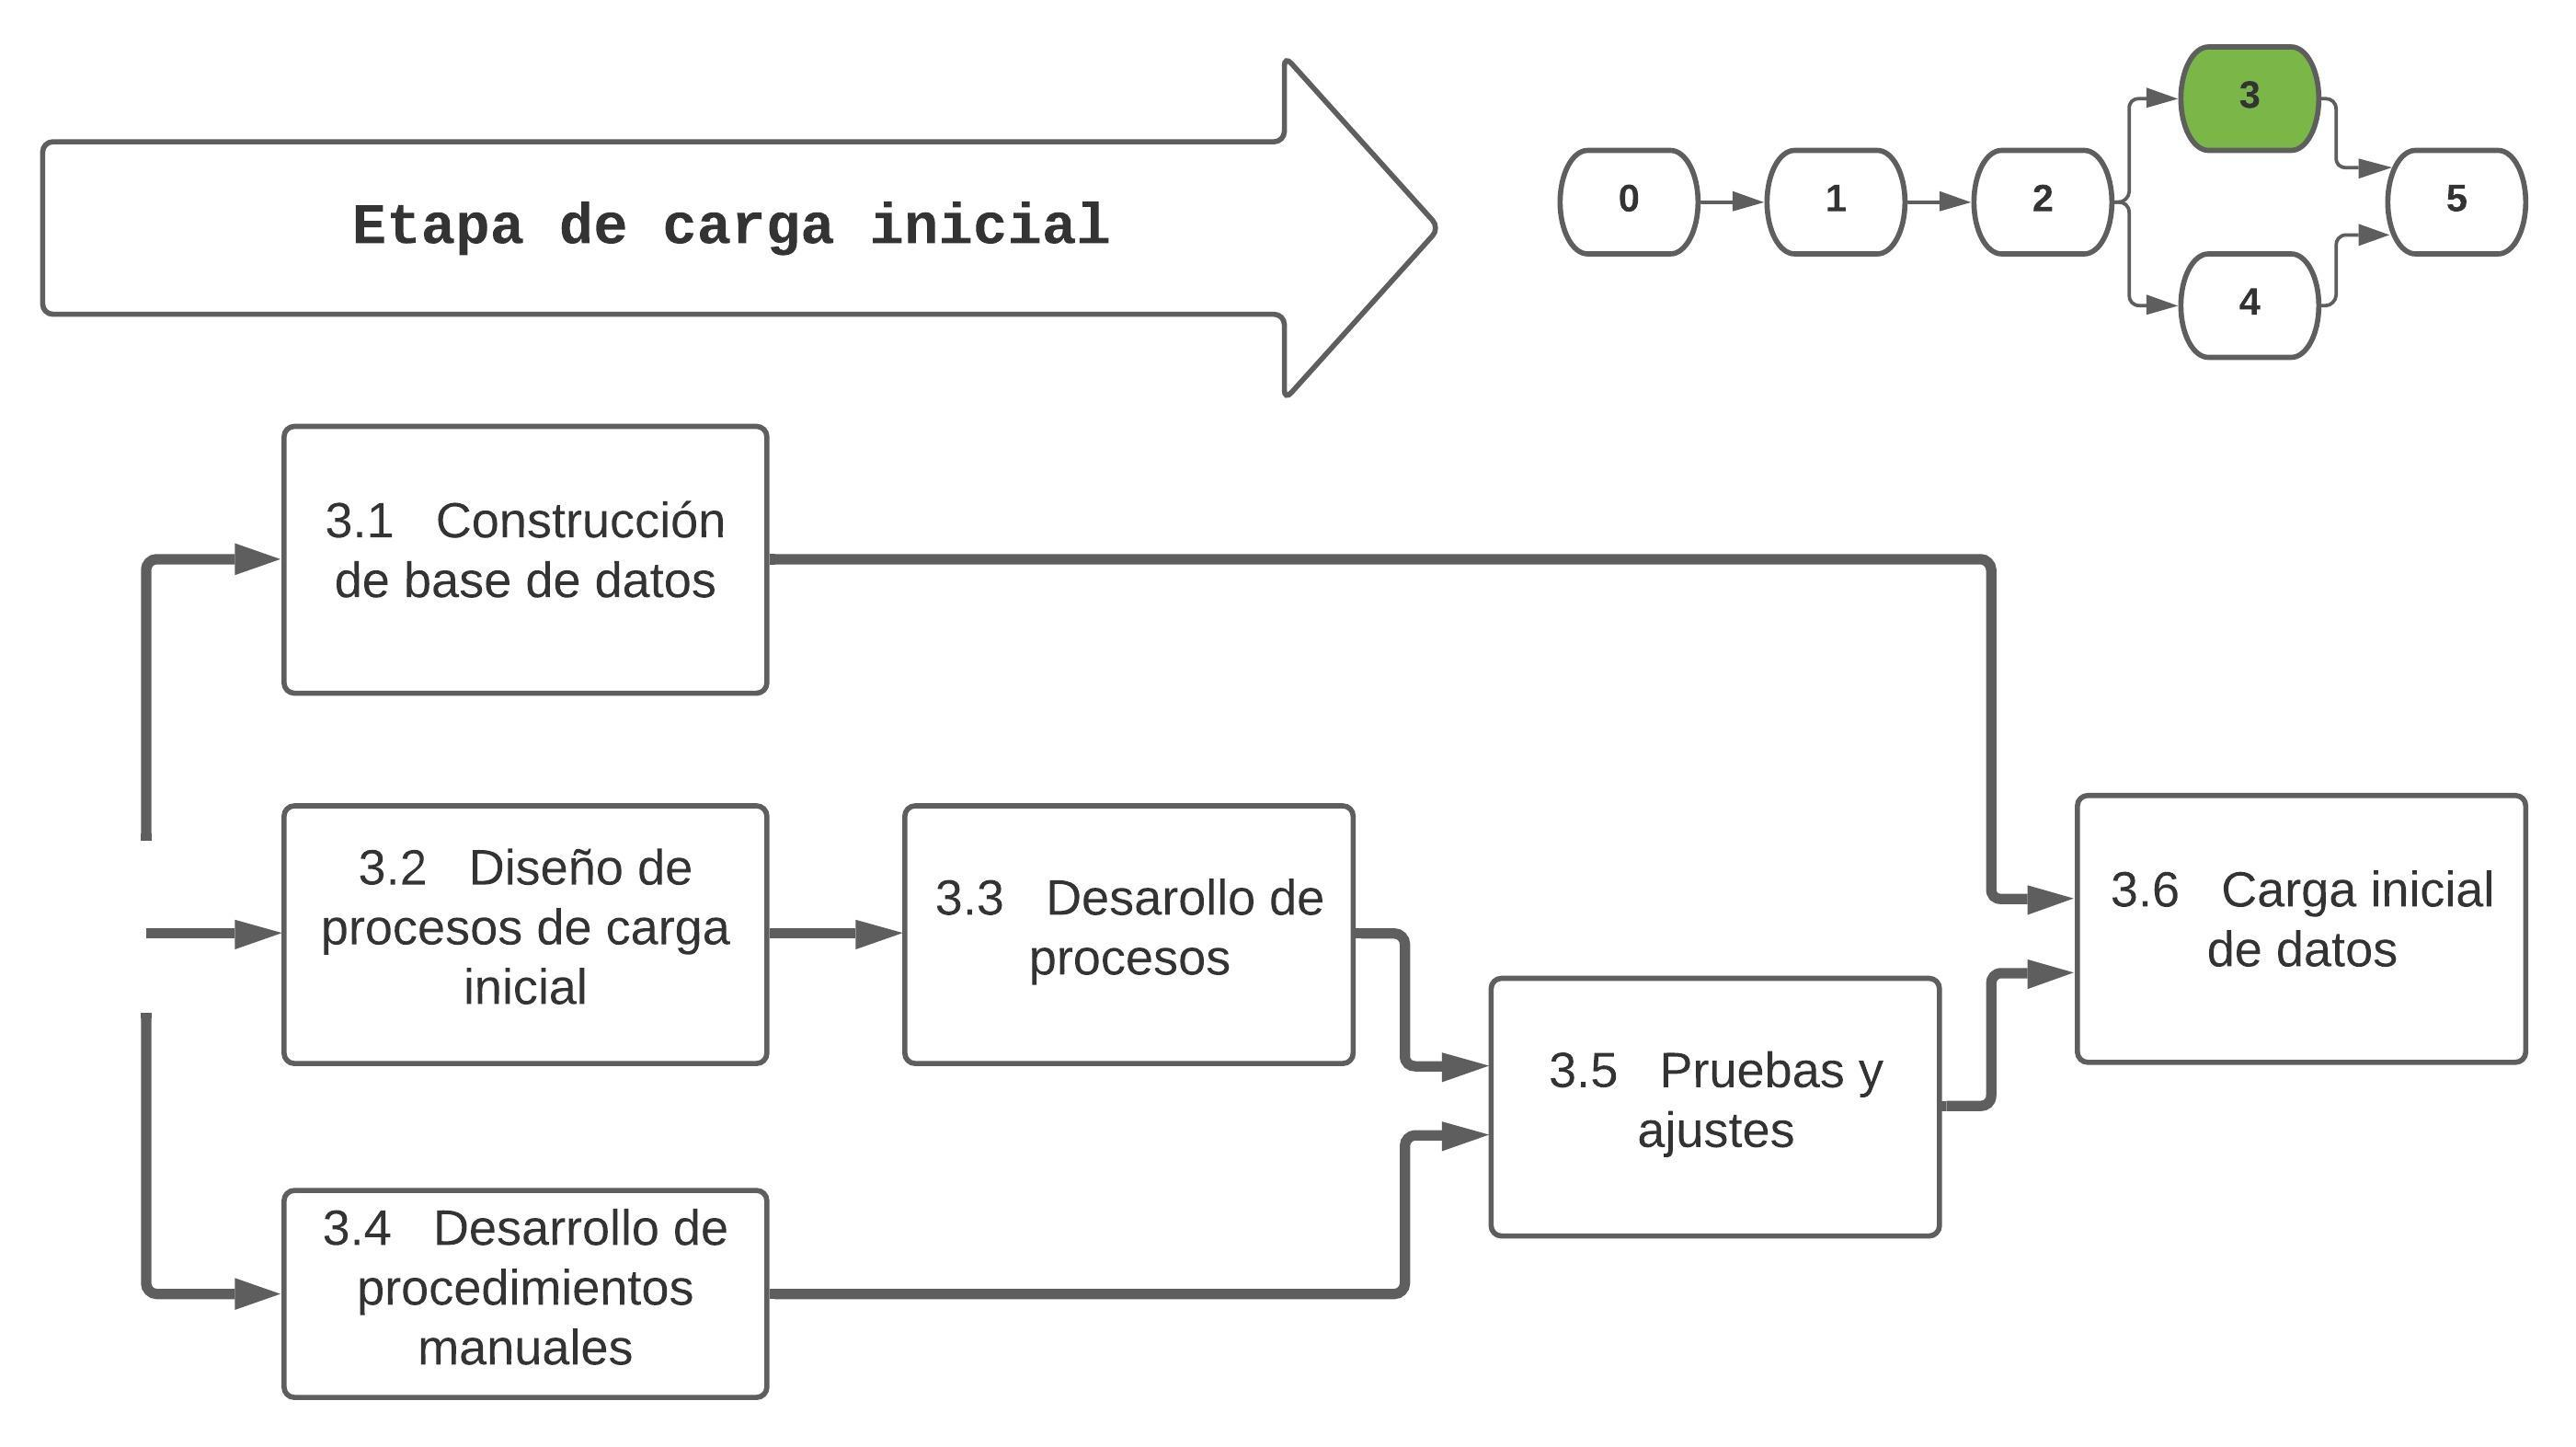
\includegraphics[width=1\linewidth]{Figuras/etapa3}
	\caption{Proceso metodológico de extracción inicial de datos. [Fuente: Propia]}
	\label{fig: etapa3}
\end{figure}

Los componentes del proceso metodológico que integran la etapa de extracción inicial de datos se describen, a continuación:

\subsubsection{Construcción de base de datos} 
Hace referencia al procedimiento de crear la base de datos que soportará cada Data Mart (DM) que integre el Data Warehouse (DWH).

\subsubsection{Diseño de carga inicial} 	
Se refiere la validación de diseños del proceso de carga inicial que contiene el mapeo de los datos requeridos, a partir de las fuentes de información.

\subsubsection{Desarrollo del proceso} 
En esta componente se considera desarrollar los procesos específicos para integrar la información en el deposito de datos.

\subsubsection{Procedimientos manuales} 
El desarrollo de procedimientos manuales es la creación de nuevos procesos no
automatizados.

\subsubsection{Pruebas a ajustes} 
Es esencial preparar un set de datos para hacer pruebas a ajustes de manera que podamos reducir el riesgo de la mínima calidad de datos.

\subsubsection{Carga inicial de datos} 
Es el procedimiento de llevar al deposito de datos toda la información histórica socializada con los usuarios finales.	


%-------------------------------------------------------------
\subsection{Actualización periódica}
Es el proceso de retroalimentación de información de producción periódica en cada Data Mart de diferentes fuentes de datos, según los procesos de carga descritos en la etapa del modelamiento de datos. Este proceso metodológico es una adaptación de Kimball (2008) y se resume en la Figura \ref{fig: etapa4}.

\begin{figure}[h]
	\centering
	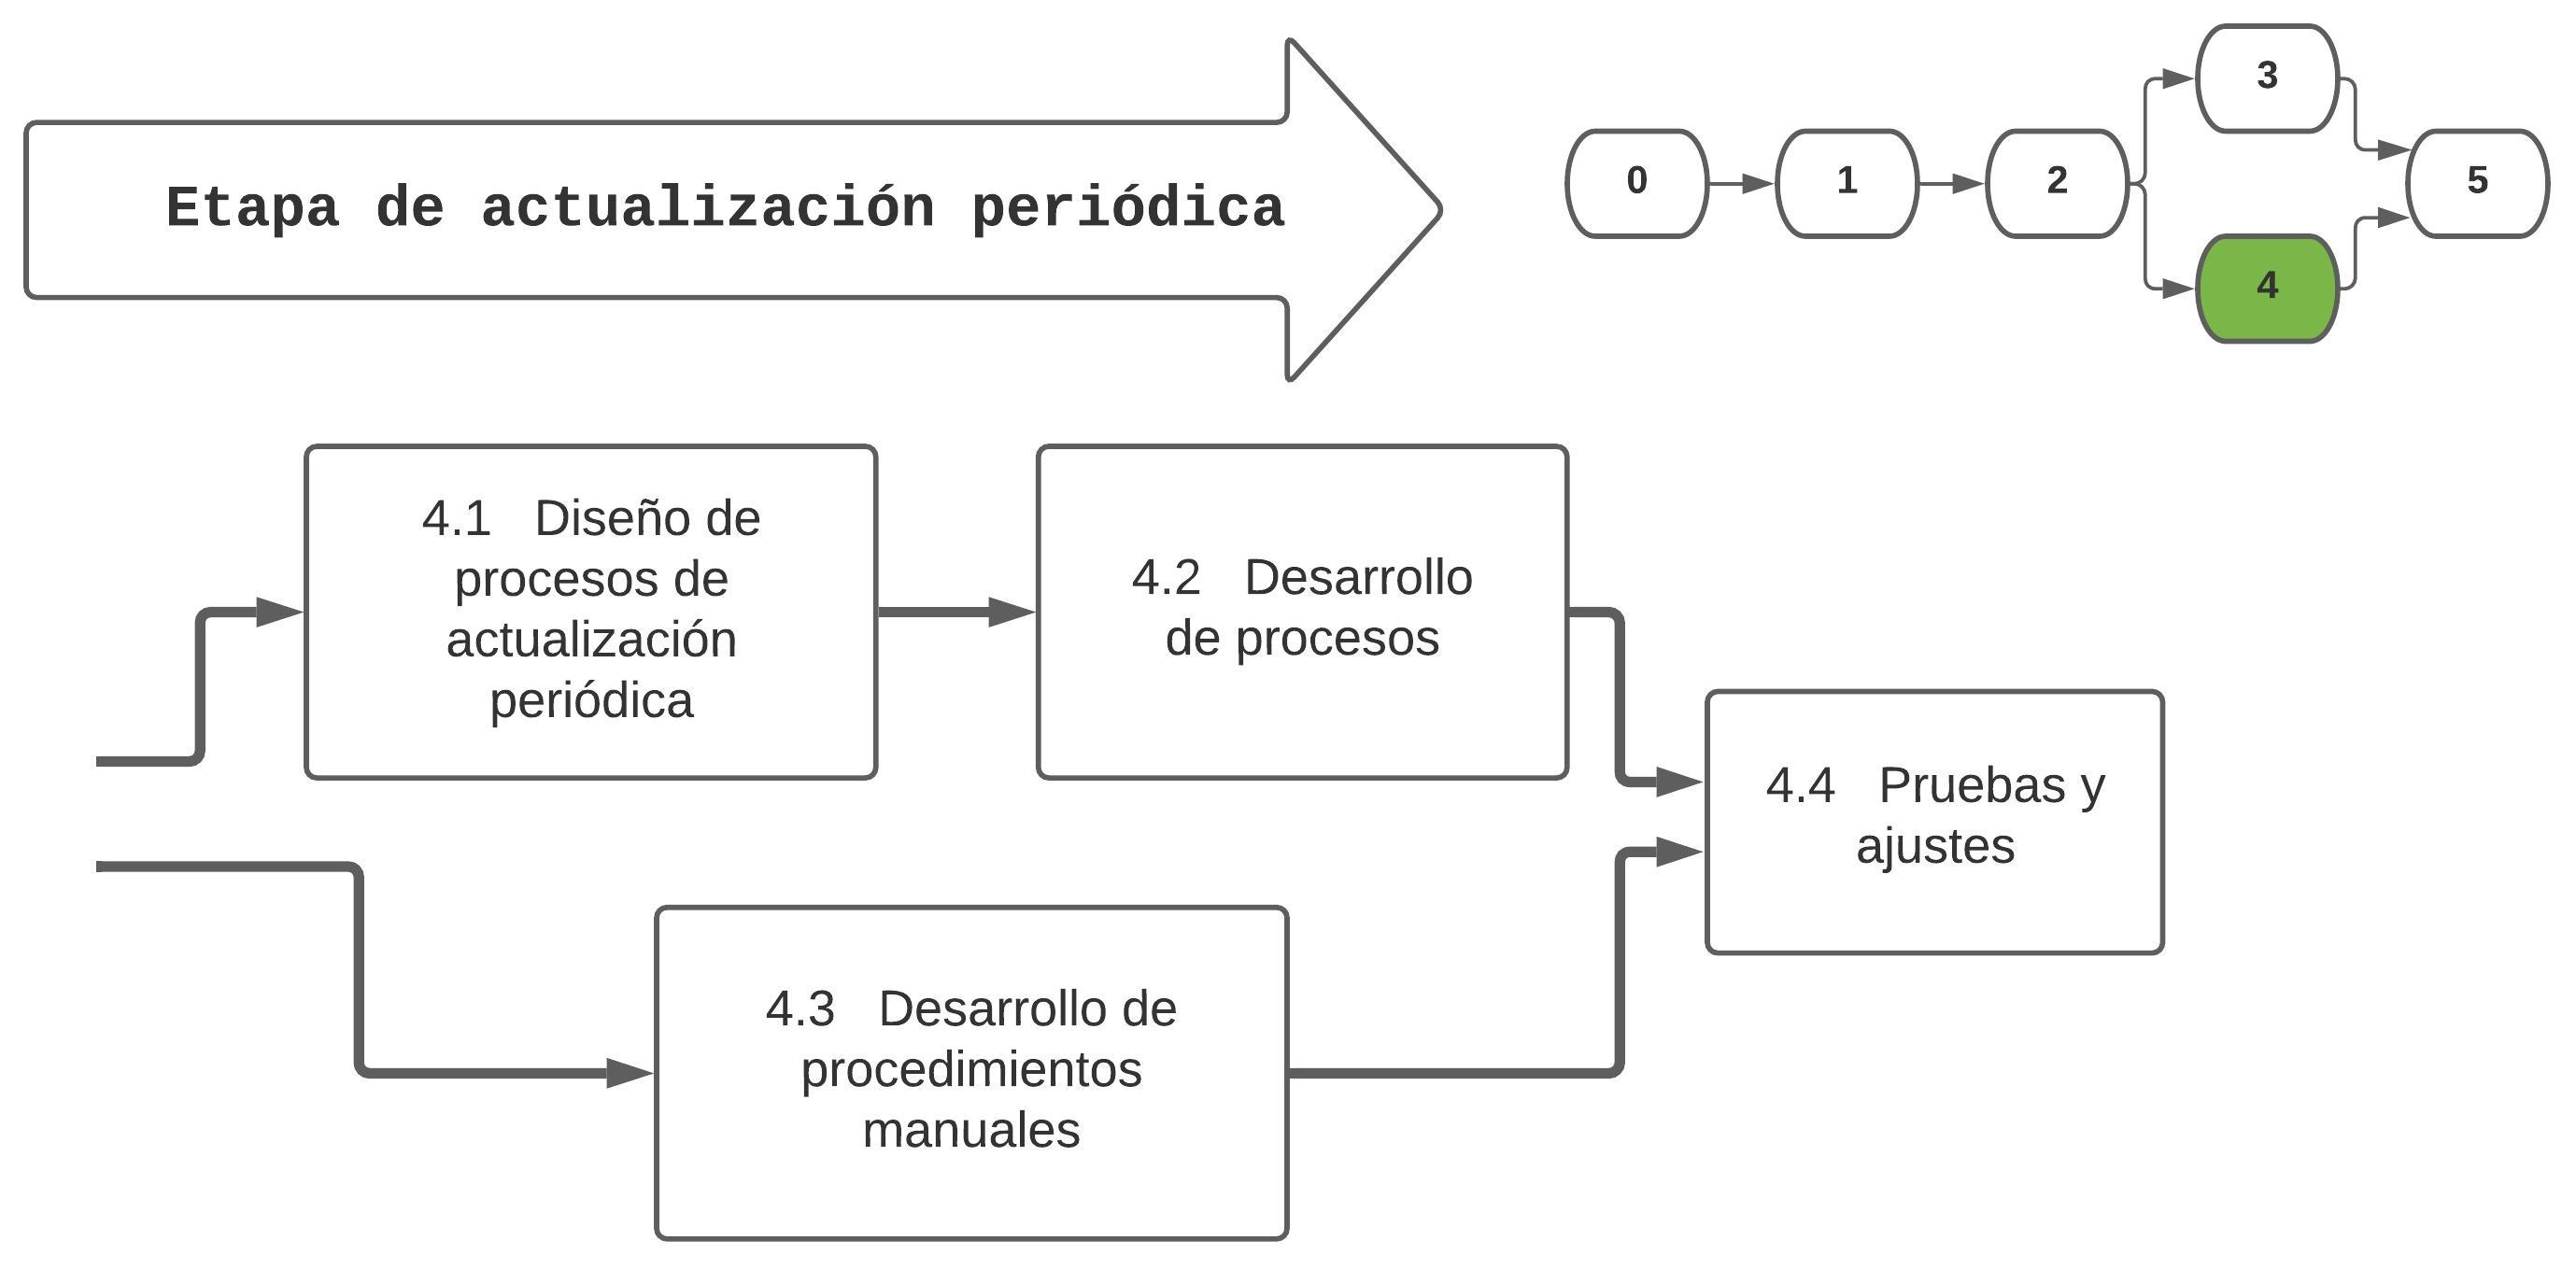
\includegraphics[width=1\linewidth]{Figuras/etapa4}
	\caption{Proceso metodológico de actualización periódica de datos. [Fuente: Propia]}
	\label{fig: etapa4}
\end{figure}

\subsubsection{Diseño de actualización periódica}
En esta etapa, el diseño del proceso de actualización periódica hace referencia a la validación de diseños de los procesos de carga periódica que contiene el mapeo de los datos requeridos, a partir de las fuentes de información.

%-----------------------------------------------------------------

\subsection{Explotación de información} 
A partir de los modelos dimensionales utilizando información histórica y transaccional, se desarrollan los aplicaciones de visualización de información, tales como: informes, consultas dinámicas y cuadros de mando. Luego, se difunde la información para su explotación, es decir, realizar la toma de decisiones. Este proceso metodológico que describe la etapa de explotación de la información es una adaptación de Kimball (2008) y se resume en la Figura \ref{fig: etapa5}.

\begin{figure}[h]
	\centering
	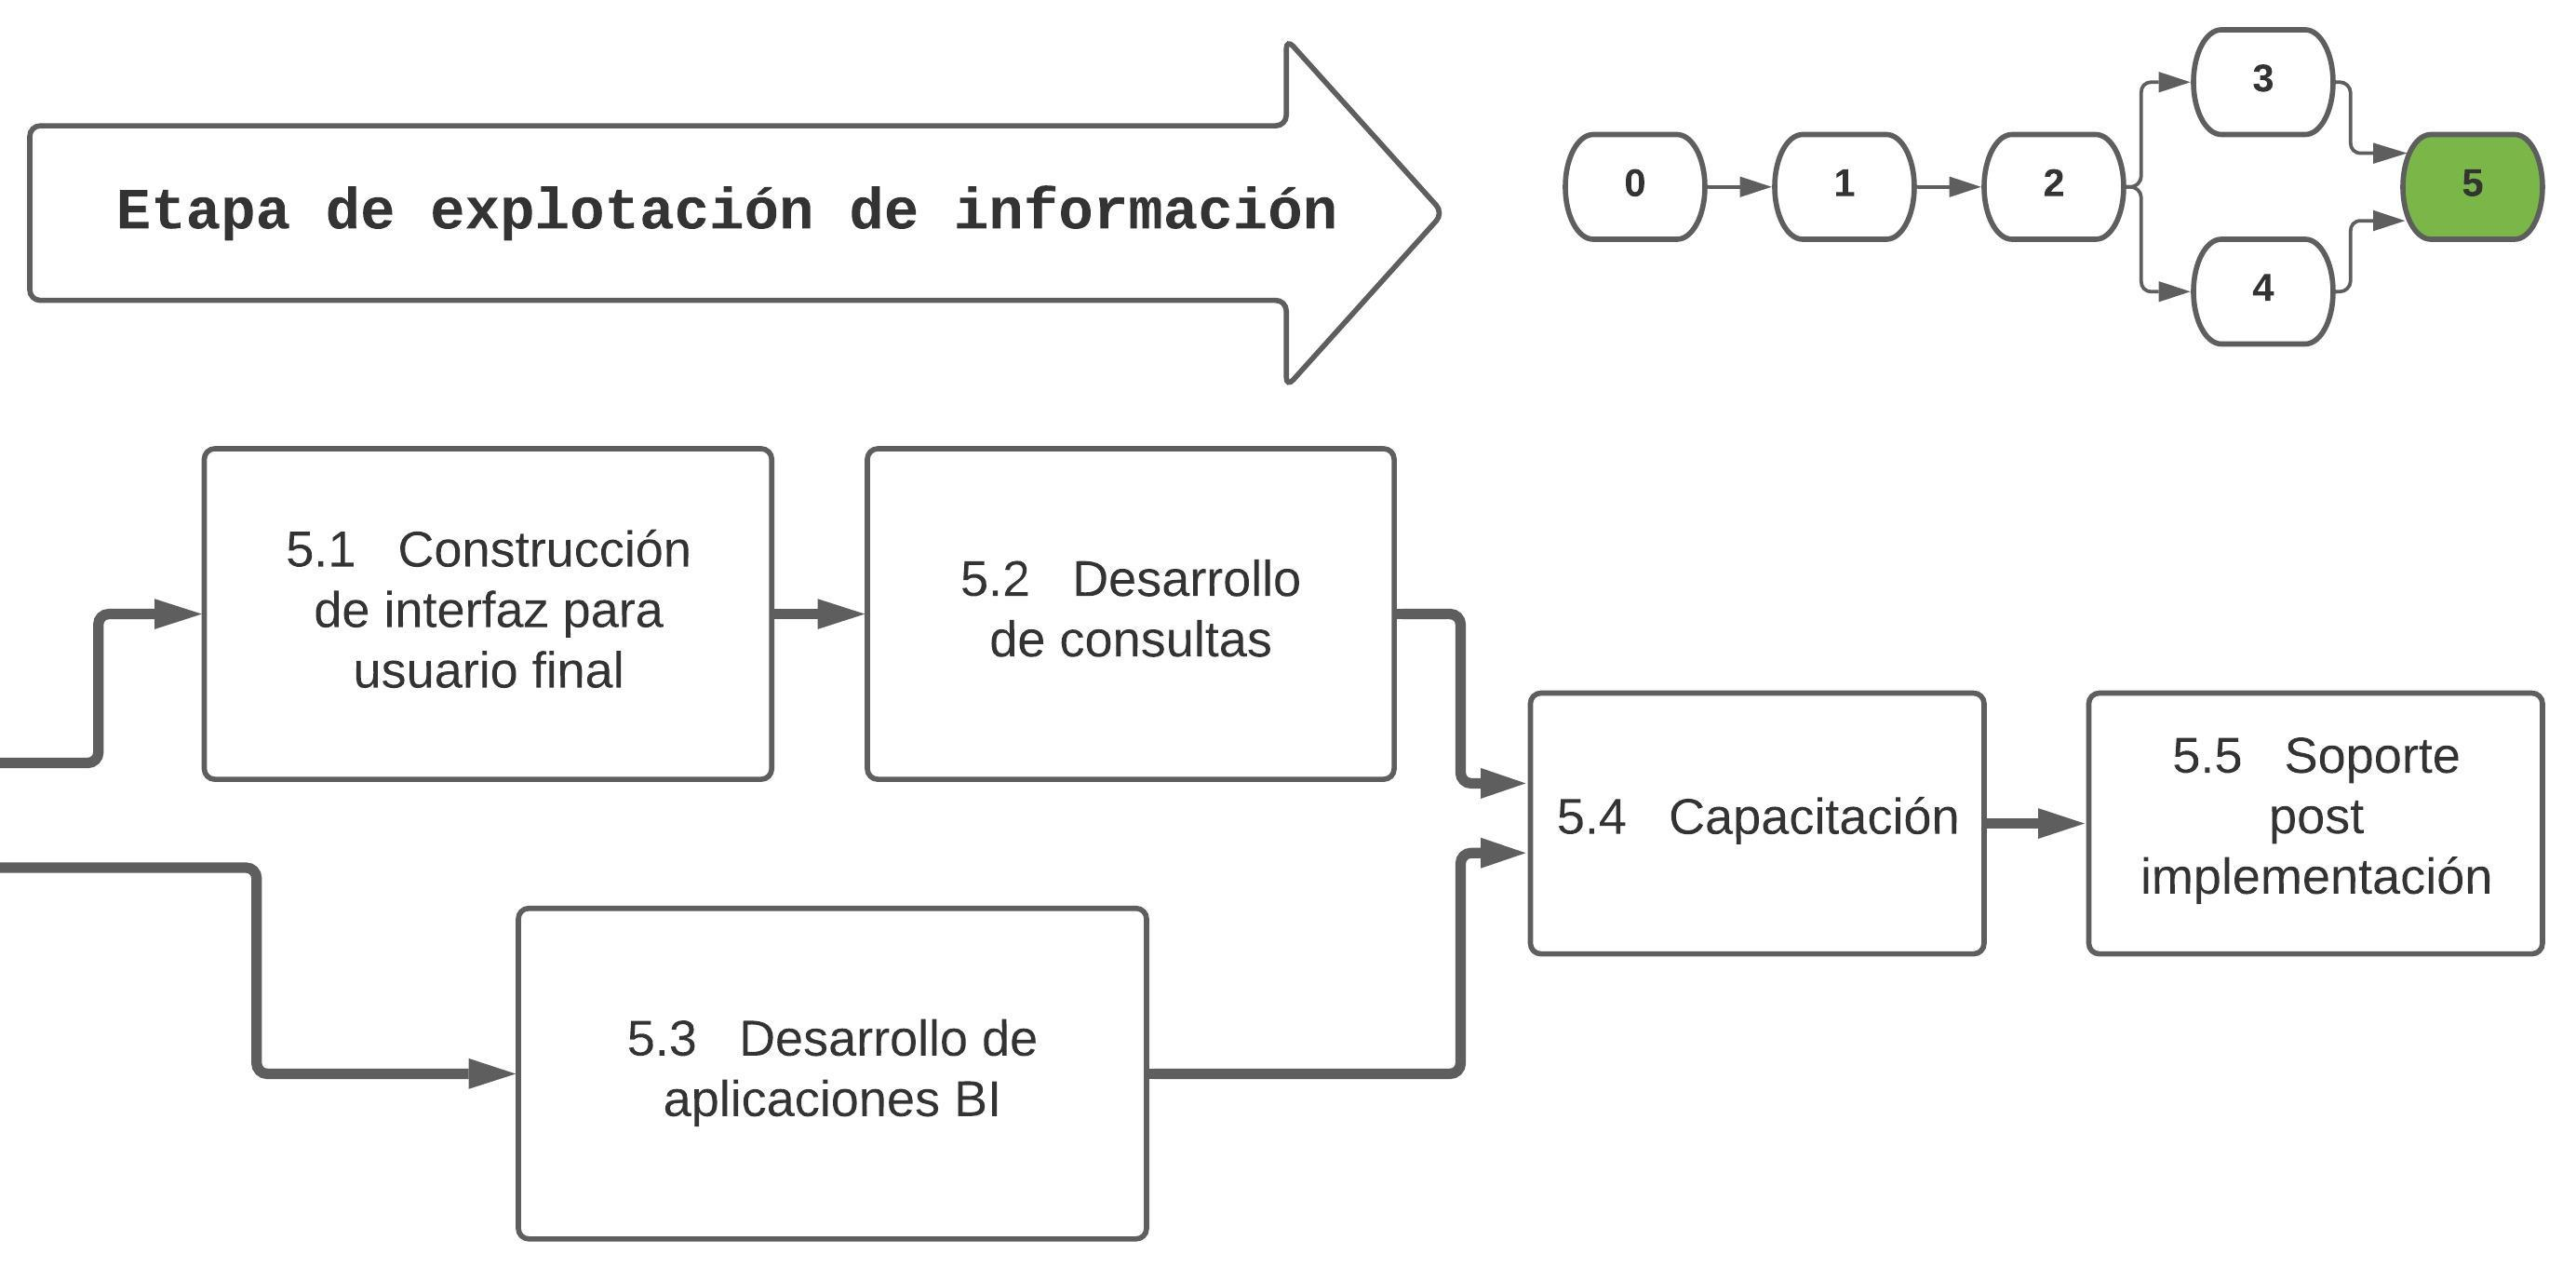
\includegraphics[width=1\linewidth]{Figuras/etapa5}
	\caption{Proceso metodológico de explotación de información. [Fuente: Propia]}
	\label{fig: etapa5}
\end{figure}

\subsubsection{Interfaz de usuario final} 
Inicialmente, en la etapa de explotación se diseña la interfaz de usuarios finales y se elaboran actividades de preparación de la plataforma tecnología, por ejemplo, se buscan los procesos que ahorran complejidad técnica al usuario final.

\subsubsection{Desarrollo de procesos}
Dentro de las estrategias de BI en las organizaciones, es prioridad considerar las herramientas de analítica de datos para seleccionar las aplicaciones. Principalmente, esto se refiere a reportes analíticos, cuadro de mandos y consultas generados mediante herramientas analíticas. Una analítica es una técnica diseñada para resolver problemas planteados mediante metamodelos genéricos o preguntas en base a situaciones cualitativas o cuantitativas, y tienen soporte en algoritmos analíticos (motores), de los cuales se describen algunos, a continuación:

\begin{description}

\item[Análisis de sets]
Este algoritmo proporciona al usuario final una segmentación de la información de manera dinámica y posteriormente, interpretar los informes. 

\item[Análisis de series temporales] 
Este análisis le permite al usuario analizar las series de tiempo simplificando
la complejidad técnica que implican sus procedimientos de visualización de datos.

\item[Reglas de los negocios]
Las aplicaciones BI deben proporcionar una manera fácil para la definición de las reglas de los negocios que le dan seguimiento a actividades desatendidas como algunos indicadores, de manera que se generan alertas de aviso al usuario y se configura la automatización de tareas (WF).
\end{description}



%  ********************************
%    MARCO PRÁCTICO 
%%%%%%%%%%%%%%%%%%%%%%%%%%%%%%%%%%%

\chapter{MARCO PRÁCTICO}

Con la finalidad de validar la investigación, en este capitulo se pretende desarrollar un prototipo de proyecto BI denominado <<cuadro de mando universitario>> que utiliza diferentes procesos metodológicos, tales como: cuadros de mando integral (BSM), modelado dimensional de datos (Cubo) y modelado analítico, entre otros.\\

En general, el prototipo es un modelo no experimental, es decir que no se manipulan variables. Por otra parte, la recopilación de datos se realizo de manera transversal (una única vez). De la misma manera, es descriptivo debido a que se pretende encontrar los efectos de los datos en la comunidad académica de manera estratégica para convertir la información en conocimiento.\\


%  ********************************
%    CONTROL DE MANDOS UNIVERSITARIO
%%%%%%%%%%%%%%%%%%%%%%%%%%%%%%%%%%%
\newpage
\section{Cuadro de mando universitario}

En perspectiva, con las aplicaciones BI se busca dar seguimiento a las actividades académicas y soporte a la toma de decisiones estratégicas u operativas alineando las estrategias académicos con las iniciativas de BI. El propósito, es validar el uso de las herramientas, aplicaciones y tecnologías aplicando los conceptos descritos en el capitulo anterior.\\

En el contexto académico, BI hace referencia al proceso de convertir la información en conocimiento para aprovechar de la mejor manera posible los recursos académicos disponibles en cada unidad administrativa u operativa. En efecto, se pretende resumir los datos más relevantes, sin tener que escribir complicadas consultas, ni participar frecuentemente en actividades de análisis de datos.\\

Intuitivamente, cada parte interesada desarrollará cierto interés en el tema de la medición. Por ejemplo, los estudiantes potenciales que deben elegir una carrera y universidad, necesitan tener referencias y soporte de comparación utilizando indicadores institucionales mediante la medición de los datos (macrodatos) en las universidades.\\

En decir, los alumnos quieren entender cuáles son sus posibilidades de obtener un buen empleo, luego de su graduación. De la misma manera, el personal docente requiere evaluar sus actividades cada cierto periodo de tiempo para mejorar la eficiencia y el personal administrativo necesita justificar el presupuesto de gastos, entre otras necesidades de información por parte de usuarios finales \cite{web08}.\\

En efecto, para satisfacer las necesidades de información en las diferentes unidades administrativas de una universidad, es importante administrar el rendimiento utilizando metodologías que gestionen los procesos universitarios.\\


\subsection{Gestión de procesos universitarios}
Con la finalidad de comprender los procesos del negocio, se puede esquematizar los modelos que permiten la gestión de los procesos académicos. Particularmente, se puede ilustrar la construcción de un modelo visual de los principales procesos en una universidad. Esto apoya a hacer más eficiente la selección sobre los indicadores (KPIs) y dar seguimiento a la estrategia de la universidad. Esta idea, se ilustra con un ejemplo de procesos académicos, en la Figura \ref{fig: ProcesoU}.

\begin{figure}[h]
\centering
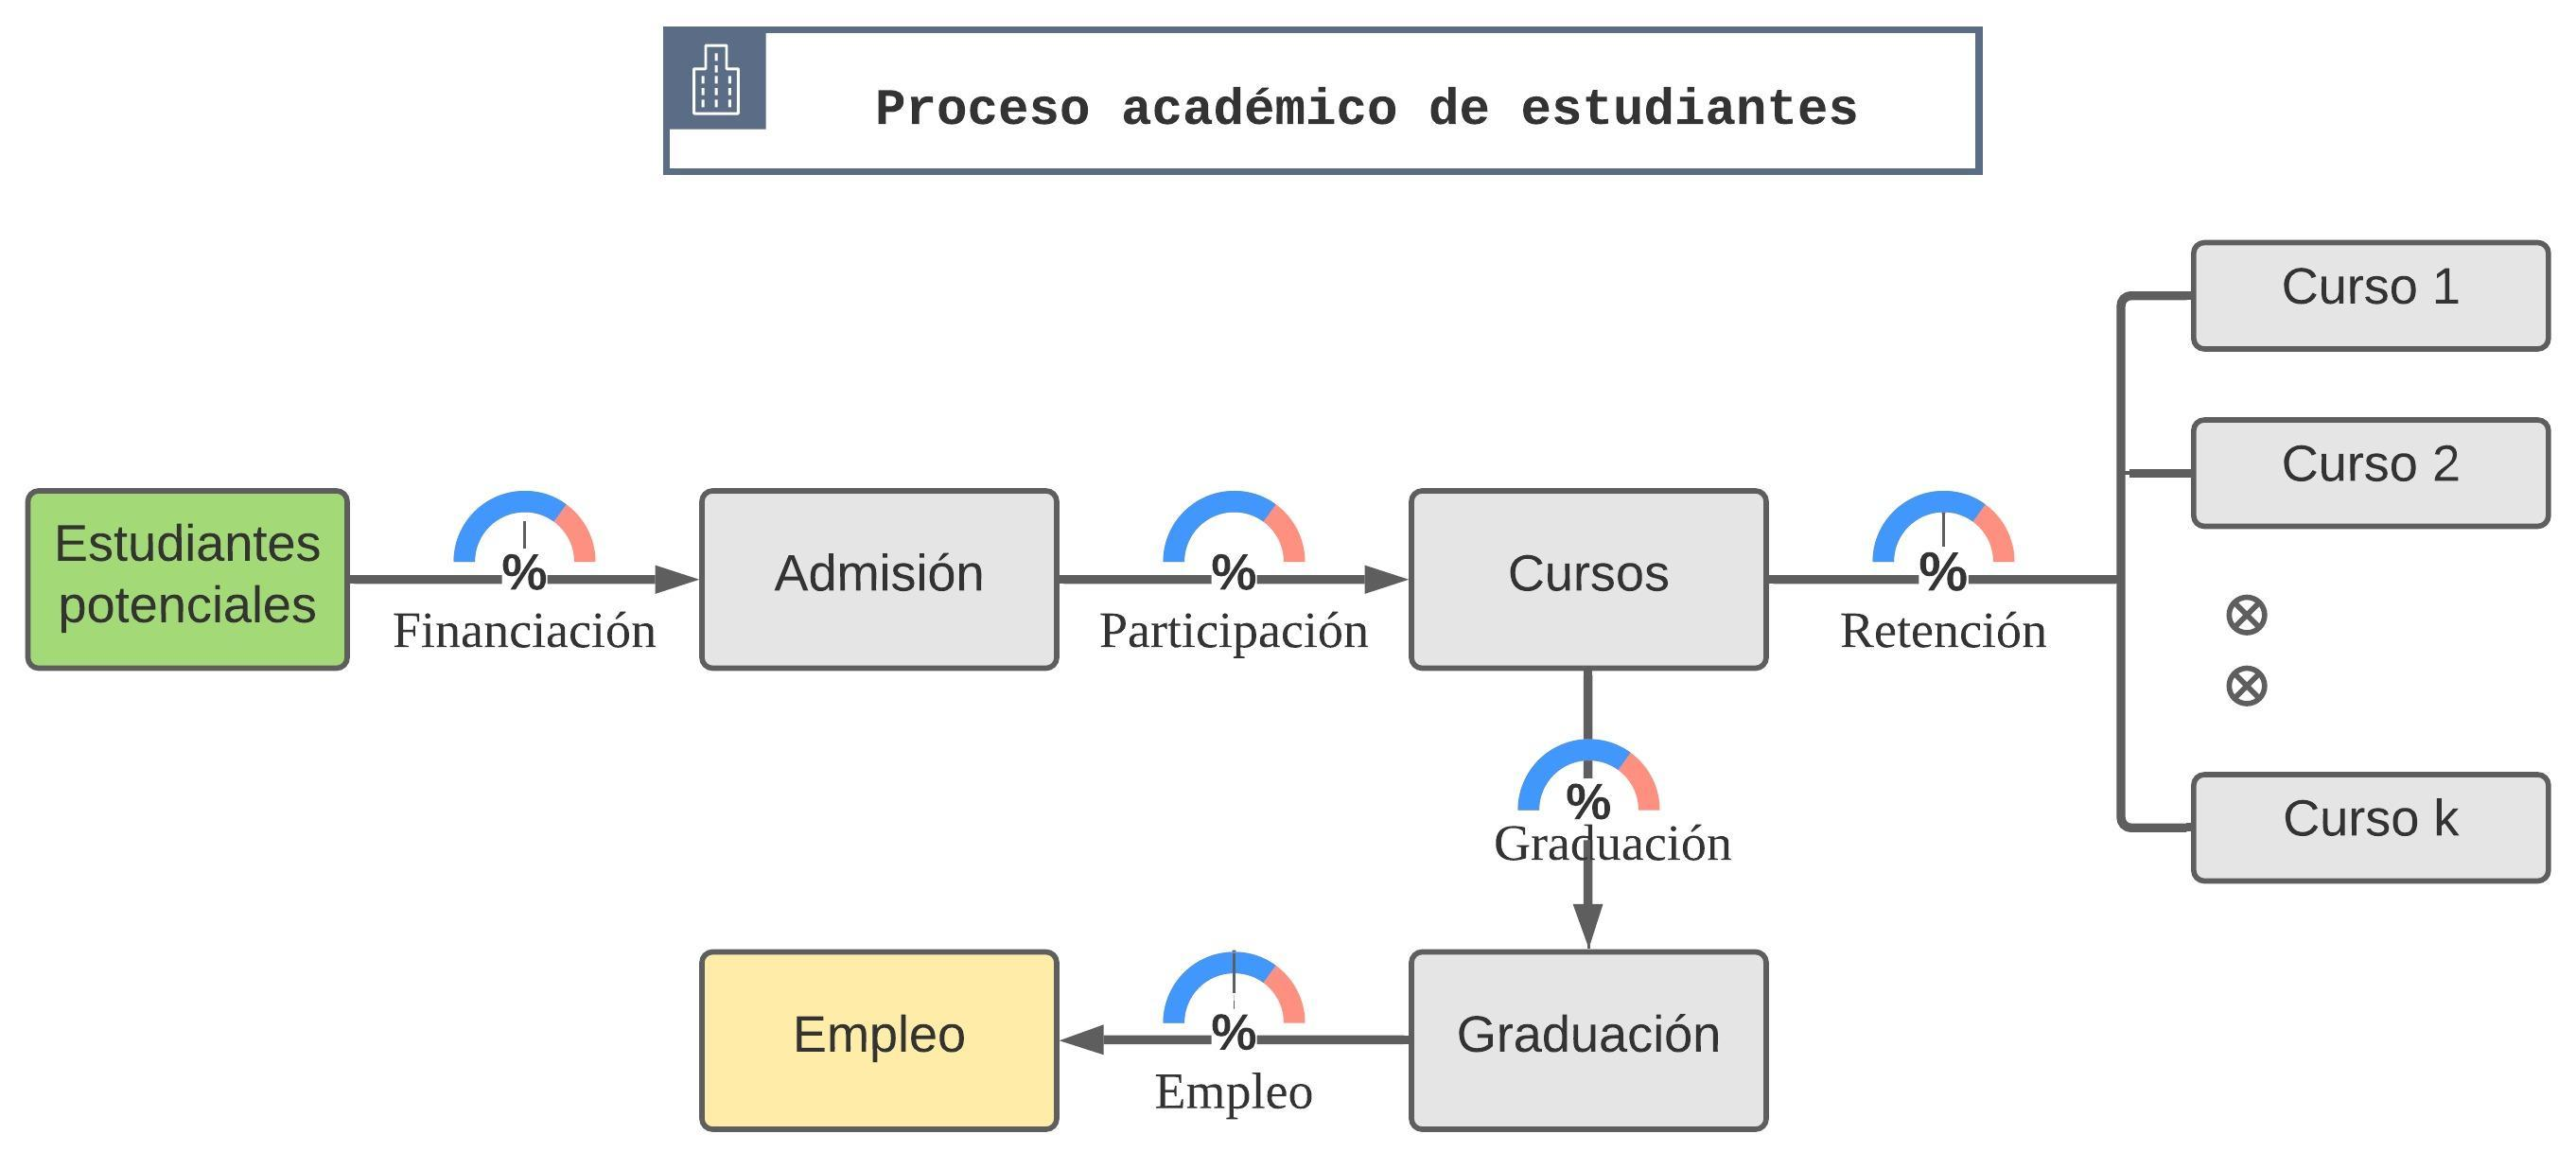
\includegraphics[width=1\linewidth]{Figuras/ProcesoU}
\caption{Ejemplo de procesos académicos. [Fuente: Propia]}
\label{fig: ProcesoU}
\end{figure}

La gestión de procesos incluye aplicaciones BI y prácticas como las siguientes:
\begin{itemize}
\item Definición de objetivos
\item Visualización de datos
\item Medición del rendimiento
\item Control administrativo u operativo 
\item Reporte diario
\item Mejoramiento de la gestión
\end{itemize}



%  ********************************
%    HERRAMIENTAS 
%%%%%%%%%%%%%%%%%%%%%%%%%%%%%%%%%%%

\section{Herramientas}

Es esencial utilizar una herramienta que permita exponer consultas e informes de manera dinámica, precisa y relevante para la toma de decisiones efectiva. Específicamente, los lenguajes de programación son muy útiles para el tratamiento de los datos. Además, del uso de programas propios del área del inteligencia de negocios (BI) utilizados para desarrollar actividades de análisis de datos.\\

 En particular, se destacan algunos programas de análisis de datos y lenguajes de programación de uso libre (open source), segun \cite{web00} los cuales se describen a continuación:

\begin{description}
\item[Power BI: ] su objetivo es proporcionar visualizaciones interactivas para que los usuarios finales puedan diseñar sus propios informes y cuadros de mando. A su vez, como variante este programa permite utilizar el lenguaje DAX (Data Analysis Expressions) para mejorar el modelo de datos y el lenguaje interactivo por defecto M.

\item[Pentaho Kettle: ] es una herramienta BI de análisis de datos que permite realizar procesos de limpieza ETL de los datos. Además, puede generar informes y aplicar minería de datos.

\item[Tableau: ] es un programa de visualización de datos interactivos centrada en la inteligencia empresarial. Además, permite analizar y compartir información en forma rápida y flexible.


\item[Python: ] es un lenguaje de programación interpretado, el cual nos permite utilizar todas las características de un lenguaje dinámico y multiplataforma. En efecto, será nuestra herramienta seleccionada para desarrollar el prototipo.

\item[R: ] es un entorno y lenguaje de programación con un enfoque al análisis estadístico. Además, es uno de los lenguajes más utilizados en investigación científica, minería de datos, biomédica y matemáticas financieras.

\item[SQL: ] es un lenguaje de consultas de bases de datos diseñado para administrar y recuperar información de los sistemas de gestión de bases de datos relacionales.\\ 

\end{description}

%  ********************************
%    IMPLEMENTACIÓN DE METODOLOGÍA BI 
%%%%%%%%%%%%%%%%%%%%%%%%%%%%%%%%%%%

\section{Implementación de metodología estándar}

Considerando la metodología estándar propuesta en el capitulo anterior y basado en el planteamiento del problema. En particular, se pretende desarrollar la aplicación de cuadro de mando universitario, este se centra en gestionar la información académica de los estudiante de una universidad mediante un modelo visual.

\subsection{Planificación del proyecto}
Con la finalidad de comprender las iniciativas de BI para una universidad, inicialmente se explora la teoría sobre estudios de directrices, especialmente de la visión y estrategias de las universidades. 

\subsubsection{Alineación de estrategias académicas}
Inicialmente, para definir el proceso principal de la planificación por parte del planificador de recursos (ERP), el cual será alinear las estrategias académicas con las iniciativas de BI mediante un sistema de medición del rendimiento (BSM). Como alternativa, se puede alinear una estrategia utilizando un enfoque basado en datos que realiza una segmentación de los estudiantes (clientes) en tres grupos: estudiantes potenciales, actuales y ex alumnos. Asimismo, seria conveniente segmentar por otros grupos involucrados como el personal académico y administrativo.\\


\subsubsection{Datos académicos}
Con el propósito de identificar los problemas de datos académicos y simplificarlos, es conveniente socializar las expectativas por parte de jefes de departamentos y coordinadores de cada facultad, con la finalidad de plantear la gestión de los recursos operativos. De la misma manera, se debe entrena el equipo para diseñar el cuadro de mando universitario (prototipo), en aspectos técnicos y funcionales para mejorar las iniciativas de BI.

\subsubsection{Plataforma Tecnológica}
En base a condición de disponibilidad de recursos académicos y del equipo tecnológico, se puede desarrollar un proyecto exitoso en las universidades. Adicionalmente, el alcance del proyecto permite restringir las necesidades de información por parte del personal académico, en el mínimo caso se espera desarrollar el modelo de gestión del proceso universitario de estudiantes (prototipo) descrito en este capitulo.\\

En la parte practica, se desarrolla el tratamiento de los datos mediante la herramienta de análisis de datos Power BI. Básicamente, se aprovecha su plataforma tecnológica disponible en la nube para difundir y explotar los informes y cuadros de mando.

\subsection{Requerimientos académicos}

Durante el proceso recurrente de recepción y evaluación de requerimientos se llevan a cabo reuniones por parte de usuarios de la organización que normalmente, se trata de director(a) de escuela, jefe(a) de departamento, coordinador(a), administrador(a) y el personal docente para socializar las necesidades de información con el equipo de planificación de recursos de BI.

\subsubsection{Selección de datos}
En resumen, los requerimientos de información académica nos permiten seleccionar los KPIs más comunes, entre los cuales se destacan en la mayoría de los cuadros de mando universitarios:
\begin{description}
\item[* Tasa de participación:]
Porcentaje de cierto grupo de la población entre los estudiantes.
\item[* Tasa de retención:]  
Retenidos en el estudio según la medición de curso a curso.
\item[* Tasa de graduación:]
El porcentaje que han completado con éxito su formación.
\item[* Éxito de empleo:]
Alumnos que obtienen un empleo luego de graduarse
\end{description}

En general, la mayoría de universidades coinciden con algunos indicadores de uso frecuente, tales como: costo promedio anual, tasa de graduación, salario después de graduarse, reputación académica, reputación del empleador, citas por facultad y tasa de estudiantes internacionales \cite{web08}. Burke y  Minassianos (2002) revisó algunos informes públicos del rendimiento de las universidades y encontró 158 indicadores KPIs. De estos, 8 indicadores fueron utilizados por más del 50\% de las universidades, los cuales se describen a continuación:

\begin{multicols}{2}
\begin{itemize}
\item Ayuda económica
\item Resultados de prueba de admisión
\item Matrícula
\item Inscripción de cursos
\item Graduación
\item Investigación patrocinada
\item Transferencias de alumnos
\item Grados otorgados
\end{itemize}
\end{multicols}

Asimismo, en las áreas claves se identificaron las mediciones más populares de los cuadros de mando, los cuales se describen a continuación:
\begin{itemize}
	\item   Datos de gastos
	\item	Puntos de admisión
	\item	Matricula (poblaciones especiales)
	\item	Facultad-General (docentes con grado)
	\item	Tasas de graduación y retención
	\item	Participación estudiantil
	\item	Relación Estudiante/Facultad\\
\end{itemize}



\subsubsection{Identificación de áreas claves}
Alinear las estrategia académicas con las iniciativas de BI, permite identificar las áreas claves de oportunidad y así, definir una estrategia coherente. Por ejemplo, la Universidad de Greenwich clasifico los KPIs en 4 perspectivas: educación (aprendizaje),  investigación, comunidad (programas) y servicios.\\

Por supuesto, las universidades no son una línea de producción. Es decir, las mediciones estándar no tendrán en cuenta valores intangibles y las clasificaciones son demasiado generales, por tanto, los informes no son útiles para realizar un proceso.\\

 En conclusión, la gerencia necesita decidir sobre un sistema de gestión del desempeño de tal forma que se pueda hacer seguimiento a las partes involucradas en la ejecución de la estrategia de las universidades. Tener una larga lista de mediciones no es suficiente para una gestión eficiente y eficaz del rendimiento. Estas perspectivas pueden ser formuladas como: estratégico, presupuesto, carrera y servicios de información \cite{web08}.\\

%  ********************************
%    FIN EVALUACIÓN DE REQUERIMIENTOS 


\subsection{Fuente de datos}
Prácticamente, la recopilación de datos se realizo en los diferentes departamentos de matemáticas de la facultad de Ciencias de la Universidad nacional Autónoma de Honduras, con la finalidad de analizar los datos disponibles de forma aislada, se cuenta como población solamente asignaturas del plan de estudios de facultad, adicionalmente datos de matricula y graduación.\\

En resumen, se partió de los resultados finales de asignaturas de una muestra y documentos antiguos, los cuales están en hojas de cálculo tipo Excel y fuentes de datos no estructuradas, respectivamente, y son producto de evaluaciones realizadas durante varios trimestres entre los periodos académicos de 2017 a 2020, por parte de docentes de la carrera de matemáticas.\\


\subsection{Modelo de datos}
Para desarrollar el proceso de transformación se utilizo la lógica del cubo tridimensional. Específicamente, se toman las tres dimensiones: matricula, asignatura y graduación en los ejes X, Y, Z, respectivamente. En efecto, se refiere a las tres tablas dimensionales que se integran para formar el modelo de datos general, luego de realizar la etapa de procesos ETL.\\

%  ********************************
%    ANALISIS DE DATOS 
%%%%%%%%%%%%%%%%%%%%%%%%%%%%%%%%%%%

\section{Análisis de datos}
En retrospectiva, con el modelo de datos se pretende desarrollar aplicaciones BI utilizando técnicas y algoritmos de analitica de datos (DA), en fin, presentar análisis de datos utilizando herramientas de visualización de la información.\\

Es decir, como producto final se obtienen los diferentes análisis de datos presentados a través de informes y cuadros de mando con una interfaz visual y dinámica, que permite explotar la información para realizar la toma de decisiones. 
En el desarrollo del prototipo se diseño una interfaz dinámica del informe y del cuadro de mando universitario, con el propósito de presentar las aplicaciones más relevantes en las unidades o departamentos de las universidades.

\subsection{Informe dinámico}
En efecto, la interfaz del informe se presenta información detallada sobre las asignaturas utilizando estadísticos comunes de las universidades, como se muestra en la Figura \ref{fig: ReporteE}.

\begin{figure}[h]
	\centering
	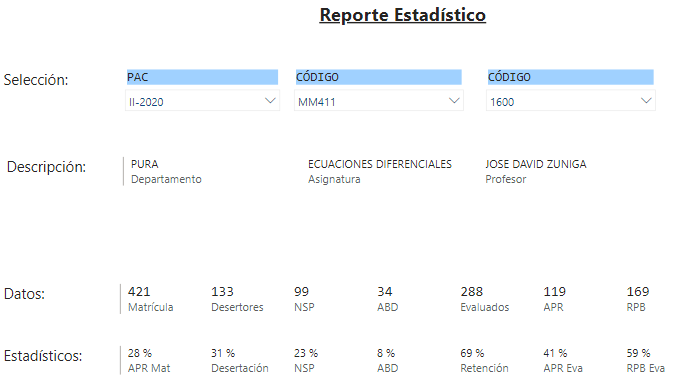
\includegraphics[width=1\linewidth]{Figuras/ReporteE}
	\caption{Reporte dinámico de asignaturas. [Fuente: Propia]}
	\label{fig: ReporteE}
\end{figure}

\subsection{Cuadro de mando universitario}
La interfaz del cuadro de mando universitario resume el diseño del esquema utilizado para alinear objetivos en el proceso universitario de estudiantes, desde la dimensión matricula hasta la de graduación. A su vez, presenta aplicaciones BI de la dimensión asignaturas, tales como: gráfico de columna agrupada y linea, gráfico de dispersión y estructura de árbol para mostrar datos jerárquicos con rectángulos, como se muestra en la Figura \ref{fig: cuadroMando}.\\

\begin{figure}[h]
	\centering
	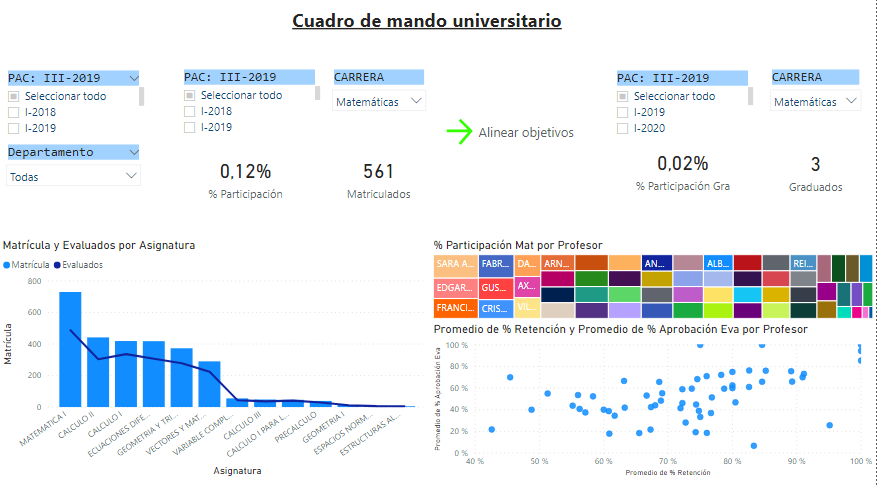
\includegraphics[width=1\linewidth]{Figuras/cuadroMando}
	\caption{Reporte dinámico de asignaturas. [Fuente: Propia]}
	\label{fig: cuadroMando}
\end{figure}


%  ********************************
%    VALIDACIÓN 
%%%%%%%%%%%%%%%%%%%%%%%%%%%%%%%%%%%

\section{Explotación de los datos}

En consecuencia del análisis de datos, se pretende difundir la información compartida en la plataforma, en esté caso se trata de la nube de Power BI, donde se dispone de todos los atributos y permisos configurados para los usuarios finales y se aprovechan todas las ventajas de su uso. Finalmente, se explota la información por parte de los gerentes, ejecutivos y usuarios de la información utilizando los informes y cuadros de mando dinámicos para realizar la toma de decisiones estratégica, táctica y operativa.


%  ********************************
%    CONCLUSIONES Y SUGERENCIAS 
%%%%%%%%%%%%%%%%%%%%%%%%%%%%%%%%%%%

\section{Conclusiones}

Se puede aprovechar el conocimiento descrito en la información de los datos para generar ventajas competitivas en las organizaciones utilizando las herramientas, aplicaciones y tecnologías de inteligencia de negocios.\\

Los metamodelos generativos nos permiten plantear problemas de situaciones cualitativas y cuantitativas mediante preguntas lógicas que se pueden responder con el análisis de datos.\\

La estructura tecnológica de una solución de inteligencia de negocios permite comprender el alcance de su implementación, de acuerdo al planteamiento del problema. Técnicamente, el propósito es explotar la información de manera dinámica, para mejorar la toma de decisiones.\\

El modelado dimensional es una técnica estructural de datos que propone integrar la información de los sistemas operacionales en depósitos de datos y analizarlos, a partir del modelo desnormalizado. De modo contrario, el modelo entidad-relación requiere datos normalizados.\\

Una solución de inteligencia de negocios, depende en gran parte del proceso metodológico y del planteamiento del problema. Sin embargo, es importante considerar el enfoque metodológico para desarrollar un proyecto exitoso.\\

La inteligencia de negocios permite desarrollar un entorno en el que soporta los procesos empresariales integrando diferentes modelos que gestionan la información de las fuentes de datos. Por tanto, los usuarios deben participar en actividades de inteligencia empresarial y desarrollar una cultura basada en los datos.\\

El cuadro de mando universitario permite describir la retroalimentación de procesos académicos para alinear la estrategia de la universidad con las iniciativas de inteligencia de negocios, utilizando procesos específicos de la administración del rendimiento académico.



 








%  ********************************
%    BIBLIOGRAFIA 
%%%%%%%%%%%%%%%%%%%%%%%%%%%%%%%%%%%
\chapter{BIBLIOGRAFÍA}
En esta investigación se llevo a cabo la lectura de diferentes ediciones de literatura, tales como: libros, artículos académicos y científicos, guías practicas, revistas académicas, foros y paginas de soporte tecnológico. A su vez, se tomó algunos cursos de análisis de datos para la toma de decisiones, ciencia de datos, informática e inteligencia de negocios.


\bibliographystyle{amsplain}
\begin{thebibliography}{12}

%%%%%%%%%%%%%%%%%% LIBROS DE TEXTO %%%%%%%%%%%%%%%%%%%%%%%%%%%%%%%
\section{Libros de Texto}

%\bibitem{aa00} Nombre Autor (Tipo, 20), \textit{ Titulo }, Edición , Capitulos , Institución, Ciudad, País.

\bibitem{lib01} Josep Curto D. y Jordi Conesa (Libro, 2010), \textit{ Introducción al Business Intelligence}, Editorial UOC, de esta edición, Barcelona, España.

\bibitem{lib02} Luis Joyanes A. (Libro, 2019), \textit{ Inteligencia de negocios y analítica de datos. Una visión global de Business Intelligence \& Analytics}, Edición , Alfaomega, Bogotá, Colombia.

\bibitem{lib03} Efraim Turban (Libro, 2014), \textit{ Business Intelligence }, 2nd Edición, Pearson College Div.

\bibitem{lib04} Ralph Kimball y otros (Libro, 2008), \textit{ The Data Warehouse Lifecycle Toolkit. Practical Techniques for Building Data Warehouse and Business Intelligence }, 2da Edición, ed. Indiana: John Wiley \& Sons, USA.

\bibitem{lib05} Alberto Cairo (Libro, 2013), \textit{ The Functional Art: an introduction to information graphics and visualization}, New Riders, USA.

%%%%%%%%%%%%%%%%%%%%%%%%% ARTICULOS ACADEMICOS %%%%%%%%%%%%%%%%%%%%%%
\section{Artículos Académicos}

%\bibitem{aa00} Nombre Autor (Tipo, 20), \textit{ Titulo }, Edición , Capitulos , Institución, Ciudad, País.

\bibitem{gui01} Medina La Plata (Guía, 2015), \textit{ Business Intelligence. Una guía práctica }, Edición 2, Universidad Peruana de Ciencias Aplicadas (UPC), Lima, Perú.
	
\bibitem{gui02} Michael A. Schif (Guía, 2009), \textit{ Documento técnico de SAP – Business Intelligence: Una guía para medianas empresas}, USA.
	
\bibitem{art02} Cathy Vega, Sania Andrade, Vicente Guevara, José A  Quiña, (Articulo, 2012) \textit{ Business Intelligence aplicado al proceso de seguimiento de graduados de la Universidad Técnica del Norte}, Universidad Técnica del Norte, Urcuquí, Ecuador.
	
\bibitem{art03} Javier Martínez C (Revista, 2020), \textit{El poder revolucionario de los datos: ciudades, edificios y activos inteligentes}, Edición 306, Business Review, Harvard.
	
\bibitem{art04} Amauri Gutiérrez (Revista, 2020), \textit{El método científico como eje de la gestión y el análisis de datos}, Edición 26, Management \& Innovation.
	
\bibitem{art05} David Donoho (Articulo, 2015), \textit{ 50 years of Data Science }, Based on a presentation at the Tukey Centennial workshop, Princeton.
	
\bibitem{art06} Thomas H. Davenport y Randy Bean (Revista, 2018), \textit{ Big Companies Are Embracing Analytics, But Most Still Don’t Have a Data-Driven Culture}, Harvard Business Review.
	
\bibitem{tes01} Aldo C. Pedraza B (Tesis, 2018), \textit{ Inteligencia en los Negocios}, Instituto Tecnológico de Orizaba, Córdoba, España.
	
\bibitem{tes02}  Santiago Morales C (Tesis, 2019), \textit{ Metodología para procesos de inteligencia de negocios con mejoras en la extracción y transformación de fuentes de datos, orientado a la toma de decisiones }, Universitat d'Alacant - Universidad de Alicante, España.
	
\bibitem{tes03}  Leonel Villamizar G (Tesis, 2010), \textit{ Como abordar un proyecto de Business inteligence en una empresa u organización}, Universidad EAFIT, Medellín.
	

%%%%%%%%%%%%%%%%%%%%%%%%%%%%% FUENTES WEB %%%%%%%%%%%%%%%%%%%%%%%%%%%%
\section{Fuentes Web}
%\bibitem{aa01} Nombre web, \textit{ https://www.nombreweb.com/}, Secciónes.

\bibitem{web00} Wikipedia, \textit{ https://es.wikipedia.org//}
	
\bibitem{web01} TimeManager, \textit{https://www.timemanagerweb.com/}, breve-historia-del-business-intelligence
	
\bibitem{web02} Directortic, \textit{ https://www.directortic.es/}, tecnologia-2
	
\bibitem{web03} Microstrategy, \textit{ https://www3.microstrategy.com/}, business intelligence the definitive guide
	
\bibitem{web04} Egafutura, \textit{ https://www.egafutura.com/}, glosario/inteligencia-negocios.
	
\bibitem{web05} Dataprix, \textit{ https://www.dataprix.com/}, Enfoques metodológicos de Business Intelligence.
	
\bibitem{web06} Conexionesan, \textit{ https://www.esan.edu.pe/}, metodología de business intelligence
	
\bibitem{web07} Dataprix, \textit{ https://www.dataprix.com/es/}, book/export/html/242.

\bibitem{web08} Bscdesigner, \textit{ https://bscdesigner.com/es}, cmi-universitario.


\section{Cursos}
\bibitem{cu01} \texttt{02/21}, Coursera - Universidad de Míchigan, \textit{Applied Plotting, Charting \& Data Representation in Python.}
\bibitem{cu02} \texttt{12/20}, INDATA - Perú, \textit{Business Intelligence para la Analítica de Datos.}
\bibitem{cu03} \texttt{11/20}, LinkedIn Learning, \textit{Power BI esencial.}
\bibitem{cu04} \texttt{10/20}, Coursera - Universidad de Míchigan, \textit{Introduction to Data Science in Python.}
\bibitem{cu05} \texttt{10/20}, Universidad Austral - Coursera, \textit{Introducción a la programación con Python.}
\bibitem{cu06} \texttt{10/20}, Tecnológico de Monterrey - Coursera, \textit{Análisis de Datos para la toma de decisiones.}
\bibitem{cu07} \texttt{09/20}, INFOP, \textit{Base de datos MySQL.}

	
\end{thebibliography}

\newpage
\thispagestyle{empty}
\vspace*{8cm}
\textbf{Henry Ford:\\}
\begin{center}
\textit{El fracaso es una gran oportunidad para empezar otra vez con más inteligencia.}
\end{center}

% ********************************************
% **********************************
\end{document}
